% !Mode:: "Tex:UTF-8"









\documentclass[10pt,a4paper]{article}\usepackage[]{graphicx}\usepackage[]{color}
%% maxwidth is the original width if it is less than linewidth
%% otherwise use linewidth (to make sure the graphics do not exceed the margin)
\makeatletter
\def\maxwidth{ %
  \ifdim\Gin@nat@width>\linewidth
    \linewidth
  \else
    \Gin@nat@width
  \fi
}
\makeatother

\definecolor{fgcolor}{rgb}{0.345, 0.345, 0.345}
\newcommand{\hlnum}[1]{\textcolor[rgb]{0.686,0.059,0.569}{#1}}%
\newcommand{\hlstr}[1]{\textcolor[rgb]{0.192,0.494,0.8}{#1}}%
\newcommand{\hlcom}[1]{\textcolor[rgb]{0.678,0.584,0.686}{\textit{#1}}}%
\newcommand{\hlopt}[1]{\textcolor[rgb]{0,0,0}{#1}}%
\newcommand{\hlstd}[1]{\textcolor[rgb]{0.345,0.345,0.345}{#1}}%
\newcommand{\hlkwa}[1]{\textcolor[rgb]{0.161,0.373,0.58}{\textbf{#1}}}%
\newcommand{\hlkwb}[1]{\textcolor[rgb]{0.69,0.353,0.396}{#1}}%
\newcommand{\hlkwc}[1]{\textcolor[rgb]{0.333,0.667,0.333}{#1}}%
\newcommand{\hlkwd}[1]{\textcolor[rgb]{0.737,0.353,0.396}{\textbf{#1}}}%
\let\hlipl\hlkwb

\usepackage{framed}
\makeatletter
\newenvironment{kframe}{%
 \def\at@end@of@kframe{}%
 \ifinner\ifhmode%
  \def\at@end@of@kframe{\end{minipage}}%
  \begin{minipage}{\columnwidth}%
 \fi\fi%
 \def\FrameCommand##1{\hskip\@totalleftmargin \hskip-\fboxsep
 \colorbox{shadecolor}{##1}\hskip-\fboxsep
     % There is no \\@totalrightmargin, so:
     \hskip-\linewidth \hskip-\@totalleftmargin \hskip\columnwidth}%
 \MakeFramed {\advance\hsize-\width
   \@totalleftmargin\z@ \linewidth\hsize
   \@setminipage}}%
 {\par\unskip\endMakeFramed%
 \at@end@of@kframe}
\makeatother

\definecolor{shadecolor}{rgb}{.97, .97, .97}
\definecolor{messagecolor}{rgb}{0, 0, 0}
\definecolor{warningcolor}{rgb}{1, 0, 1}
\definecolor{errorcolor}{rgb}{1, 0, 0}
\newenvironment{knitrout}{}{} % an empty environment to be redefined in TeX

\usepackage{alltt}
\usepackage{etoolbox}
\newtoggle{color}
%\togglefalse{color}
\toggletrue{color}

\usepackage{makeidx}
\newcommand{\idioma}{spanish}
\newcommand{\opcionesIdioma}{,es-nodecimaldot,es-tabla}
% !Mode:: "Tex:UTF-8"
%%%%%%%%%%%%%%%%%%%%%Carga de Packages
%%poner \newcommand{\idioma}{spanish} o \newcommand{\idioma}{english} en el documento
\usepackage{pdfsync}
\usepackage{srcltx}
\usepackage[\idioma\opcionesIdioma]{babel}
\usepackage[utf8x]{inputenc}
\usepackage[T1]{fontenc}
\usepackage{graphicx}
\graphicspath{{/users/fernando/figuras/}{./}{./figuras/}{/fernando/figuras/}{/fernando/figuras/jpg/}}
\usepackage{multicol}
\usepackage{epsfig}
%\usepackage{oberdiek}
\usepackage{listingsutf8}
\lstset{inputencoding=utf8/latin1}
%\lstset{extendedchars=true}
\lstset{ %
  language=R,                     % the language of the code
  basicstyle=\ttfamily\small,       % the size of the fonts that are used for the code
  numbers=left,                   % where to put the line-numbers
  numberstyle=\tiny\color{gray},  % the style that is used for the line-numbers
  stepnumber=1,                   % the step between two line-numbers. If it's 1, each line
                                  % will be numbered
  numbersep=5pt,                  % how far the line-numbers are from the code
  backgroundcolor=\color{white},  % choose the background color. You must add \usepackage{color}
  showspaces=false,               % show spaces adding particular underscores
  showstringspaces=false,         % underline spaces within strings
  showtabs=false,                 % show tabs within strings adding particular underscores
  frame=single,                   % adds a frame around the code
  rulecolor=\color{black},        % if not set, the frame-color may be changed on line-breaks within not-black text (e.g. commens (green here))
  tabsize=2,                      % sets default tabsize to 2 spaces
  %captionpos=,                   % sets the caption-position to bottom
  breaklines=true,                % sets automatic line breaking
  breakatwhitespace=false,        % sets if automatic breaks should only happen at whitespace
  %title=\lstname,                 % show the filename of files included with \lstinputlisting;
                                  % also try caption instead of title
  keywordstyle=\color{black},      % keyword style
  commentstyle=\color{Brown},   % comment style
  stringstyle=\color{black},      % string literal style
  escapeinside={\%*}{*)},         % if you want to add a comment within your code
  morekeywords={*,...},            % if you want to add more keywords to the set
  lineskip={-2.5pt} % single line spacing
}
%\usepackage{algorithm}
\usepackage{amsmath}
\usepackage{amsfonts}
\usepackage{amssymb}
\usepackage{amsthm}
\usepackage{fancybox}
\usepackage{fancyvrb}
\usepackage{rotating}
\usepackage{keystroke}
\usepackage{array}
\input{xy}
\xyoption{all}
%\usepackage[dvipsnames,usenames]{color}
\usepackage[usenames,dvipsnames,svgnames,table]{xcolor}
\usepackage{colortbl}
\usepackage{comment}
\excludecomment{spanish}
\excludecomment{english}
\includecomment{\idioma}

%\usepackage{noweb}
%\usepackage{clrscode}
\usepackage{eurosym}
\usepackage{wasysym}
\usepackage{multirow}
%\usepackage{margins}
\usepackage{lscape}
\usepackage{longtable}
\usepackage[normalem]{ulem}
\usepackage{xr-hyper}

%%NUEVO
\newcolumntype{C}{{\centering\arraybackslash}m{20mm}}
\newcommand{\centercell}[1]{\multicolumn{1}{c}{#1}}
\newcommand{\colHead}[1]{\centercell{\bfseries#1}}

\excludecomment{ocultar}


% Matriz (par‚ntesis)
\def\matr#1#2{\left(\begin{array}{#1}#2\end{array}\right)}
% Determinante (barras)
\def\deter#1#2{\left|\begin{array}{#1}#2\end{array}\right|}
% Sistema de ecuaciones. (llave a la izda.)
\def\seq#1#2{\left\{\begin{array}{#1}#2\end{array}\right.}
% Ecuaci\'on de varias lineas (sin llave a la izda.)
\def\evl#1#2{\begin{array}{#1}#2\end{array}}

%%%%%%%%%%%%%%%%%%%%%%%%%%%%%%%%%%%%%%%%%%%%%%
%%%%%%%%%%%%%%%%%%%%%%%%%%%%%%%%%%%%%%%%%%%%%%
%%%%%%%%%%%%%%%%% M\'{a}rgenes %%%%%%%%%%%%%%%%
%
%
%\parindent=0mm
%
%\textwidth=160mm
%\textheight=220mm
%\hoffset=-20mm
%\voffset=-15mm
%\parskip=0mm
\marginparsep=3mm
\marginparwidth=25mm
%
%%%%%%%%%%%%%%%%%%%%%%%%%%%% Contadores para listas de problemas
%\newcommand{\adc}{\addtocounter{enumi}{1}}
\newcommand{\adc}{\stepcounter{enumi}}
\newcommand{\adci}{\stepcounter{enumii}}
\newcommand{\xadc}{\addtocounter{xcounter}{1}}
\newcommand{\be}{\begin{enumerate}}
\newcommand{\ee}{\end{enumerate}}
\newcommand{\bi}{\begin{itemize}}
\newcommand{\ei}{\end{itemize}}
\newcounter{xcounter}


\newcommand{\nin}{{\noindent}}

%\newcounter{prob}{}
%\def\pr{\addtocounter{prob}{1}(\theprob)\ }
%\def\pr2{\addtocounter{prob}{2}(\theprob)\ }

%%%%%%%%%%%%%%%%%%%%%%%%%%%Fin de demostraciones, ejemplos, etc.
\newcommand{\fin}{$\square$}
%%%%%%%%%%%%%%%%%%%%%%%%%%Notaci\'{o}n matem\'{a}ticas generales
%\newcommand{\suc}[1]{\{#1_n\}}
%\newcommand{\sucn}[1]{\{#1_n\}_{n\in\mathbb{N}}}
%\newcommand{\ser}[1]{\sum #1_n}
%\newcommand{\sern}[1]{\sum_{n\geq 1} #1_n}
%\newcommand{\limn}{\lim_{n\rightarrow\infty}}
%\newcommand{\limnd}{\displaystyle\lim_{n\rightarrow\infty}}
%\newcommand{\mf}[1]{\mathbf{#1}}
%\newcommand{\mb}[1]{\mathbb{#1}}
%\newcommand{\D}[1]{\Dv_{\mf{#1}}}
%\newcommand{\bsigma}{\pmb{\sigma}}
%\newcommand{\bPhi}{\pmb{\Phi}}
%\newcommand{\vol}{\operatorname{vol}}
%\newcommand{\ldbr}{[\hspace{-1.5pt}[}
%\newcommand{\rdbr}{]\hspace{-1.5pt}]}
%\newcommand{\fpws}[2]{{#1}\ldbr{#2}\rdbr}
%\newcommand{\leftPui}{<\hspace{-3pt}<}
%\newcommand{\rightPui}{\hspace{-3pt}}
%\newcommand{\Pui}[2]{{#1}\hspace{-6pt}\leftPui{#2}\rightPui}
%\newcommand{\pdd}[2]{\dfrac{\partial{#1}}{\partial{#2}}}
%%%%%%%%%%Conjuntos de n\'{u}meros
\newcommand{\N}{\mathbb{N}} %conjunto de n\'{u}meros naturales
\newcommand{\Z}{\mathbb{Z}} %conjunto de n\'{u}meros enteros
\newcommand{\R}{\mathbb{R}} %conjunto de n\'{u}meros reales
\newcommand{\C}{\mathbb{C}} %conjunto de n\'{u}meros complejos
\newcommand{\Q}{\mathbb{Q}} %conjunto de n\'{u}meros racionales
\newcommand{\EP}{\mathbb{P}} %espacios proyectivos
\newcommand{\K}{\mathbb{K}} %cuerpo gen\'{e}rico
\newcommand{\A}{\mathbb{A}} %espacios afines

%%%%%%%%%%Estadistica
\newcommand{\MEAN}{\mathrm{E}}
\newcommand{\Var}{\mathrm{Var}}
\newcommand{\Cov}{\mathrm{Cov}}


%%%%%%%%%%Funciones
\def\arcsen{\operatorname{arcsen}}
\def\arctg{\operatorname{arctg}}
\def\argCosh{\operatorname{argCosh}}
\def\argSenh{\operatorname{argSenh}}
\def\argTgh{\operatorname{argTgh}}
\def\cosec{\operatorname{cosec}}
\def\Cosh{\operatorname{Cosh}}
\def\cotg{\operatorname{cotg}}
\def\Dv{\operatorname{D}}
\def\discrim{\operatorname{discrim}}
\def\dive{\operatorname{div}}
\def\dom{\operatorname{dom}}
\def\Ext{\operatorname{Ext}}
\def\Fr{\operatorname{Fr}}
\def\dder#1#2{\dfrac{d #1}{d #2} } %derivada en estilo display
\def\gr{\operatorname{gr}}
\def\grad{\operatorname{grad}}
\def\Imag{\operatorname{Im}}
\def\mcm{\operatorname{mcm}}
\def\rang{\operatorname{rang}}
\def\rot{\operatorname{rot}}
\def\sen{\operatorname{sen}}
\def\Senh{\operatorname{Senh}}
\def\sgn{\operatorname{sgn}}
\def\sig{\operatorname{sig}}
\def\tg{\operatorname{tg}}
\def\Tgh{\operatorname{Tgh}}
\def\E{\operatorname{E}}
\def\VAR{\operatorname{VAR}}
\newcommand{\margWeb}[2]{\noindent{#2}\marginpar[\hspace{-18mm}\link{#1}{WEB}]{\hspace*{-18mm}\link{#1}{WEB}}}

%%%%%%%%%%%%%%%%%%%%%%\'{A}lgebra conmutativa.
\def\multideg{\operatorname{multideg}} %multidegree of a polynomial
\def\LT{\operatorname{lt}} %leading term of a polynomial
\def\LC{\operatorname{lc}} %leading coefficient of a polynomial
\def\LM{\operatorname{lm}} %leading monomial of a polynomial
\def\Mexp{\mathbb{Z}^n_{\geq 0}} %set of multiexponents of monomials
\def\set#1{\left\{{#1}\right\}}
\newcommand{\vlist}[2]{\mbox{${#1}_{1},\ldots,{#1}_{#2}$}}
\def\deg{\operatorname{deg}} %grado de un polinomio
\def\cp{\operatorname{cp}} %coeficiente principal de un polinomio
\def\CP{\operatorname{cp}} %coeficiente principal de un polinomio
\def\set#1{\left\{{#1}\right\}} %llaves de conjunto
\newcommand{\V}{{\bf V}} %variedad de un conjunto de polinomios
\newcommand{\I}{{\bf I}} %ideal de un conjunto
\newcommand{\MCD}{\operatorname{mcd}} %m\'{a}ximo com\'{u}n divisor
\newcommand{\MCM}{\operatorname{mcm}} %m\'{\i}nimo com\'{u}n m\'{u}ltiplo
\newcommand{\LCM}{\operatorname{lcm}} %least common multiple
\newcommand{\GCD}{\operatorname{gcd}} %greatest common divisor
\newcommand{\Ker}{\operatorname{Ker}} %N\'{u}cleo
\newcommand{\IM}{\operatorname{IM}} %Imagen
\newcommand{\Rad}{\operatorname{Rad}} %radical de un ideal
\newcommand{\Jac}{\operatorname{Jac}} %radical de Jacobson de un anillo
\newcommand{\Ann}{\operatorname{Ann}} %anulador de un ideal
\newcommand{\Res}{\operatorname{Res}} %resultante de polinomios
\newcommand{\Mult}{\operatorname{mult}} %multiplicidad
\newcommand{\Gen}{\operatorname{Gen}} %g\'{e}nero
\newcommand{\Card}{\operatorname{Card}} %cardinal
\newcommand{\ord}{\operatorname{ord}} %orden
\newcommand{\prim}{\operatorname{prim}} %parte primitiva
\newcommand{\NP}{\operatorname{NP}} %NP idea
\newcommand{\cont}{\operatorname{cont}} %parte primitva
\newcommand{\pp}{\operatorname{pp}} %parte primitva
\newcommand{\PP}{\mathop{\mathrm{PP}}\nolimits}
\newcommand{\Int}{\operatorname{Int}}
\newcommand{\Ind}{\operatorname{index}}
\newcommand{\Lcoeff}{\operatorname{lc}} %leading coefficient of a polynomial
\newcommand{\Sqf}{\operatorname{Sqf}} %square free part of a polynomial

\def\pd#1#2{\frac{\partial #1}{\partial #2}} %derivada parcial
\def\mult{\text{mult}} %multiplicity
\def\Sing{\text{Sing}} %multiplicity
\def\Cl#1{\overline{#1}} %cierre topol\'{o}gico
\def\fobox#1{\begin{center}\fbox{$\displaystyle #1 $}\end{center}}

%\newcommand{\Ext}{\operatorname{Ext}}

%%%%%%%%%%%%%%%%%%%%%%%%
%% unpunto mayor que cdot, pero menor que bullet
\newcommand{\sbt}{\,\begin{picture}(-1,1)(-1,-3)\circle*{3}\end{picture}\ }

%%%%%%%%%%%%%%%%%%%%%%%%S\'{\i}mbolos rodeados de un c\'{\i}rculo
\def\circled#1{\xymatrix{*+[o][F]{#1}}}

%%%%%%%%%%%%%%%%%%%Geometr\'{\i}a
\newcommand{\CH}{{\cal CH}} %%cierre convexo

%%%%%%%%%%%%%%%%%%%%Tipos de letra especiales
%%Caligr\'{a}ficas
\newcommand{\cA}{{\cal A}}
\newcommand{\cB}{{\cal B}}
\newcommand{\cC}{{\cal C}}
\newcommand{\cD}{{\cal D}}
\newcommand{\cE}{{\cal E}}
\newcommand{\cF}{{\cal F}}
\newcommand{\cG}{{\cal G}}
\newcommand{\cH}{{\cal H}}
\newcommand{\cI}{{\cal I}}
\newcommand{\cJ}{{\cal J}}
\newcommand{\cK}{{\cal K}}
\newcommand{\cL}{{\cal L}}
\newcommand{\cM}{{\cal M}}
\newcommand{\cN}{{\cal N}}
\newcommand{\cO}{{\cal O}}
\newcommand{\cP}{{\cal P}}
\newcommand{\cQ}{{\cal Q}}
\newcommand{\cR}{{\cal R}}
\newcommand{\cS}{{\cal S}}
\newcommand{\cT}{{\cal T}}
\newcommand{\cU}{{\cal U}}
\newcommand{\cV}{{\cal V}}
\newcommand{\cW}{{\cal W}}
\newcommand{\cX}{{\cal X}}
\newcommand{\cY}{{\cal Y}}
\newcommand{\cZ}{{\cal Z}}

%%%%%%%%%%%%%%%%%%%%%%%%%%Notaci\'{o}n matem\'{a}ticas generales
\newcommand{\sucn}[1]{\{#1_n\}_{n\in\mathbb{N}}}
\newcommand{\ser}[1]{\sum #1_n}
\newcommand{\sern}[1]{\sum_{n\geq 1} #1_n}
\newcommand{\limn}{\lim_{n\rightarrow\infty}}
\newcommand{\mf}[1]{\mathbf{#1}}
\newcommand{\mb}[1]{\mathbb{#1}}
\newcommand{\D}[1]{\Dv_{\mf{#1}}}
\newcommand{\bsigma}{\pmb{\sigma}}
\newcommand{\bPhi}{\pmb{\Phi}}
\newcommand{\vol}{\operatorname{vol}}
\newcommand{\ldbr}{[\hspace{-1.5pt}[}
\newcommand{\rdbr}{]\hspace{-1.5pt}]}
\newcommand{\fpws}[2]{{#1}\ldbr{#2}\rdbr}
\newcommand{\leftPui}{<\hspace{-3pt}<}
\newcommand{\rightPui}{\hspace{-3pt}}
\newcommand{\Pui}[2]{{#1}\hspace{-6pt}\leftPui{#2}\rightPui}
\newcommand{\pdd}[2]{\dfrac{\partial{#1}}{\partial{#2}}}


%\newcounter{contEnlace}

%\newcommand{\pendiente}{\textcolor{purple}{PENDIENTE: }}
%\newcommand{\link}[2]{\textcolor{blue}{{\href{#1}{#2}}}}


\iftoggle{color}{%
  % color version
  \newcommand{\pendiente}{\textcolor{red}{PENDIENTE: }}
  \newcommand{\link}[2]{\textcolor{blue}{{\href{#1}{#2}}}}
  \newcommand{\fichero}[2]{\textattachfile{#1}{\textcolor{blue}{#2}}}
  \newcommand{\otrofichero}[2]{\textattachfile{./datos/#1}{\textcolor{blue}{#2}}}
}{%
  % b/w version
  \newcommand{\pendiente}{\textcolor{black}{\underline{PENDIENTE:} }}
  \newcommand{\link}[2]{\textcolor{black}{{\href{#1}{\underline{#2}}}}}
  \newcommand{\fichero}[2]{\textattachfile{#1}{\textcolor{black}{\underline{#2}}}}
  \newcommand{\otrofichero}[2]{\textattachfile{./datos/#1}{\textcolor{black}{\underline{#2}}}}
}



%{\textcolor{blue}{{\href{#1}{#2}}}}

%%%%%%%%%%%%%%%%%%COLORES

\DefineNamedColor{named}{Brown}{cmyk}{0,0.81,1,0.60}
\definecolor{Gris050}{gray}{0.50}
\definecolor{Gris025}{gray}{0.75}
\definecolor{Gris010}{gray}{0.90}


%%%%%%%%%%%%%%%%%%%%%Package Algorithms
%\begin{spanish}
%\renewcommand{\algorithmicrequire}{{precondici\'{o}n:}}
%\renewcommand{\algorithmicensure}{{postcondici\'{o}n:}}
%\renewcommand{\algorithmicend}{{fin}}
%\renewcommand{\algorithmicif}{{si}}
% \renewcommand{\algorithmicthen}{{entonces}}
% \renewcommand{\algorithmicelse}{{si no}}
% \renewcommand{\algorithmicelsif}{\algorithmicelse\ \algorithmicif}
% \renewcommand{\algorithmicendif}{\algorithmicend\ \algorithmicif}
% \renewcommand{\algorithmicfor}{{para}}
% \renewcommand{\algorithmicforall}{{para todo}}
% \renewcommand{\algorithmicdo}{{hacer}}
% \renewcommand{\algorithmicendfor}{\algorithmicend\ \algorithmicfor}
% \renewcommand{\algorithmicwhile}{{mientras}}
% \renewcommand{\algorithmicendwhile}{\algorithmicend\ \algorithmicwhile}
% \renewcommand{\algorithmicrepeat}{{repetir}}
% \renewcommand{\algorithmicuntil}{{hasta}}
% \end{spanish}

%%%%%%%%%%%%%%%%%%%%%%%%%%%%%%%%%%Package Amsthm
\begin{spanish}
%\theoremstyle{definition}% default
\theoremstyle{plain}
\newtheorem{thm}{Teorema}[section]
\newtheorem{teo}{Teorema}[section]
\newtheorem{teorema}{Teorema}[section]
\newtheorem{lem}[thm]{Lema}
\newtheorem{lema}[thm]{Lema}
\newtheorem{prop}[thm]{Proposici\'{o}n}
\newtheorem{proposicion}[thm]{Proposici\'{o}n}
\newtheorem{cor}[thm]{Corolario}
\newtheorem{corolario}[thm]{Corolario}
\newtheorem*{KL}{Klein's Lemma}
%\theoremstyle{definition}
\newtheorem{defn}[thm]{Definici\'{o}n}
\newtheorem{definicion}[thm]{Definici\'{o}n}
\newtheorem{conj}[thm]{Conjetura}
\newtheorem{conjetura}[thm]{Conjetura}
\newtheorem{definicionInformal}[thm]{Definición Informal}
\newtheorem{exmp}[thm]{Ejemplo}
\newtheorem{ejemplo}[thm]{Ejemplo}
\newtheorem{Ejemplo}[thm]{Ejemplo}
\newtheorem{ejem}[thm]{Ejemplo}
\newtheorem{ejercicio}{Ejercicio}
%\theoremstyle{remark}
\newtheorem*{rem}{Observaci\'{o}n}
\newtheorem{observacion}[thm]{Observaci\'{o}n}
\newtheorem*{note}{Nota}
\newtheorem{nota}[thm]{Nota}
\newtheorem{case}[thm]{Caso}
\newtheorem{caso}[thm]{Caso}
\newtheorem{regla}[thm]{Regla}

\theoremstyle{remark}
\newtheorem{enlace}{$\bullet$ }
\end{spanish}

\begin{english}
\theoremstyle{plain}% default
%\theoremstyle{definition}
\newtheorem{thm}{Theorem}[section]
\newtheorem{lem}[thm]{Lemma}
\newtheorem{prop}[thm]{Proposition}
\newtheorem{cor}[thm]{Corollary}
\newtheorem*{KL}{Klein's Lemma}
\newtheorem{defn}[thm]{Definition}
\newtheorem{conj}[thm]{Conjecture}
\newtheorem{exmp}[thm]{Example}
\theoremstyle{remark}
\newtheorem*{rem}{Remark}
\newtheorem*{note}{Note}
\newtheorem{case}{Case}
\end{english}

%%%%%%%%%%%%%%%Package Listings
%\lstset{showstringspaces=false}
%\newcommand{\PAS}[1]{\lstinline@#1@}
%\newcommand{\CPP}[1]{\lstinline@#1@}


%%%%%%%%%%%%Estilo para bibliograf\'{\i}a

%\bibliographystyle{plain}

%%%%%%%%%%%%Mis anotaciones
\newcommand{\Pendiente}[1]{\textcolor{red}{Pendiente: #1}}
%\newcommand{\Pendiente}{\textcolor{purple}{Pendiente: }}

\newcommand{\fernando}[1]{\textcolor{red}{Fernando: #1}}

%%%%%%%%%%%%%%%% Enlace al indice
%\renewcommand{\chaptermark}[1]{\markboth{\chaptername\ \thechapter.#1 \ref{index}}{}}

%%%%%%%%%%%%%%%%%%Traducci\'{o}n de clrscode
%\renewcommand{\For}{\textbf{Para} }
%\renewcommand{\To}{\textbf{hasta} }
%\renewcommand{\By}{\textbf{incremento} }
%\renewcommand{\Downto}{\textbf{downto} }
%\renewcommand{\While}{\textbf{mientras} }
%\renewcommand{\Repeat}{\textbf{repetir}\\\addtocounter{indent}{1}}
%\renewcommand{\Until}{\kill\addtocounter{indent}{-1}\liprint\\\textbf{hasta que}\hspace*{-0.7em}\'}
%\renewcommand{\If}{\textbf{si} }
%\renewcommand{\Then}{\\textbf{entonces}\hspace{13mm}\\addtocounter{indent}{1}}
%\renewcommand{\Else}{\kill\addtocounter{indent}{-1}\liprint\\textbf{sino}\\addtocounter{indent}{1}}
%\renewcommand{\End}{\addtocounter{indent}{-1}}
%\renewcommand{\ElseIf}{\kill\addtocounter{indent}{-1}\liprint\textbf{sino si} }
%\renewcommand{\ElseNoIf}{\kill\addtocounter{indent}{-1}\liprint\textbf{si no}\addtocounter{indent}{1}}
%\renewcommand{\Do}{\\\textbf{hacer}\hspace*{-0.7em}\'\addtocounter{indent}{1}}
%\renewcommand{\Return}{\textbf{devolver} }
%\renewcommand{\Comment}{$\hspace*{-0.075em}\rhd$ }
%\renewcommand{\RComment}{\`\Comment}
%\renewcommand{\Goto}{\textbf{Ir a} }
%\renewcommand{\Error}{\textbf{error} }


%%%%%%%%%%%%%%%%%%%%%%%%%%%%%%%%%%%%%%%%%%%%%%%%%%%%%%%%%%%%%%%
%Cabecera para ejercicios
%\documentclass[11pt]{article}
%\newcommand{\idioma}{spanish}
%\input definiciones
%
%\textwidth=160mm \textheight=240mm \hoffset=-20mm \voffset=-30mm
%%\parskip=0mm
%%\marginparsep=-25mm \evensidemargin=82pt\evensidemargin=44pt
%
%
%\includecomment{solucion}
%%\excludecomment{solucion}

%%Compatibilidad con documentos antiguos
\newcounter{prob}{}
\def\pr{\noindent\addtocounter{prob}{1}(\theprob)\ }
\def\bepro{ \setcounter{prob}{0}}

%%Compatibilidad con documentos antiguos
% \def\ojo#1{
% \noindent$\btr$#1
% \marginpar[
% {GeoGebra}]
% {GeoGebra}}

% \def\atencion#1{\noindent #1
% \marginpar[
% {\includegraphics*[scale=1,width=1.2cm,keepaspectratio=true]{./datos/hipoizda}}]
% {\includegraphics*[scale=1,width=1.2cm,keepaspectratio=true]{./datos/hipodcha}}}


\def\Rlogo#1{\noindent #1
\marginpar[
{\includegraphics*[scale=1,width=1.5cm,keepaspectratio=true]{./datos/Rlogo.jpg}}]
{\includegraphics*[scale=1,width=1.5cm,keepaspectratio=true]{./datos/Rlogo.jpg}}}

\def\calcLogo#1{#1}

%\def\calcLogo#1{\noindent #1
%\marginpar[
%{\includegraphics*[scale=1,width=1.2cm,keepaspectratio=true]{./datos/LogoHojaCalculo.png}}]
%{\includegraphics*[scale=1,width=1.2cm,keepaspectratio=true]{./datos/LogoHojaCalculo.png}}}


\def\ninja#1{\noindent #1
\marginpar[ {\includegraphics*[scale=1,width=1.2cm,keepaspectratio=true]{../fig/ninja_desk.png}}]
{\includegraphics*[scale=1,width=1.2cm,keepaspectratio=true]{../fig/ninja_desk.png}}}

\def\buda#1{\noindent #1
\marginpar[ {\includegraphics*[scale=1,width=1.2cm,keepaspectratio=true]{../fig/Computer-Buddha.png}}]
{\includegraphics*[scale=1,width=1.2cm,keepaspectratio=true]{../fig/Computer-Buddha.png}}}


\def\puffin#1{\noindent #1
\marginpar[ {\includegraphics*[scale=1,width=1.2cm,keepaspectratio=true]{../fig/frailecillo3.png}}]
{\includegraphics*[scale=1,width=1.2cm,keepaspectratio=true]{../fig/frailecillo3-dcha.png}}}


\def\atencion{
\marginpar[
{\includegraphics*[scale=1,width=2cm,keepaspectratio=true]{./datos/hipoizda}}]
{\includegraphics*[scale=1,width=2cm,keepaspectratio=true]{./datos/hipodcha}}}


\def\ojo#1{
\noindent #1
\marginpar[
{\includegraphics*[scale=1,width=1.5cm,keepaspectratio=true]{./datos/hipoojoi}}]
{\includegraphics*[scale=1,width=1.5cm,keepaspectratio=true]{./datos/hipoojod}}}

\def\ojo2{
\marginpar[
{\includegraphics*[scale=1,width=1.5cm,keepaspectratio=true]{./datos/hipoojoi}}]
{\includegraphics*[scale=1,width=1.5cm,keepaspectratio=true]{./datos/hipoojod}}}


\def\lio#1{
\noindent$\btr$#1
\marginpar{\includegraphics*[scale=1,width=1.1cm,keepaspectratio=true]{./datos/hipolio}}}

\def\cuentas{
\marginpar{\includegraphics*[scale=1,width=1.3cm,keepaspectratio=true]{./datos/hipocuen}}}

\def\pensar{
\marginpar{\includegraphics*[scale=1,width=1.5cm,keepaspectratio=true]{./datos/hipopens}}}

\def\facil{
\marginpar{\includegraphics*[scale=1,width=2cm,keepaspectratio=true]{./datos/hipofcil}}}



\newcommand{\WikipediaLogo}{\marginpar{\includegraphics*[scale=1,width=1.2cm,keepaspectratio=true]{./datos/LogoWikipedia}}}
\newcommand{\MoodleLogo}{\marginpar{\includegraphics*[scale=1,width=1.2cm,keepaspectratio=true]{./datos/MoodleLogo}}}
\newcommand{\WirisGeoGebraLogo}{\marginpar{\includegraphics*[scale=1,width=1.2cm,keepaspectratio=true]{./datos/WirisGeoGebraLogo}}}
\newcommand{\WirisLogo}{\marginpar{\includegraphics*[scale=1,width=1.2cm,keepaspectratio=true]{./datos/WirisLogo}}}
\newcommand{\GeoGebraLogo}{\marginpar{\includegraphics*[scale=1,width=1.2cm,keepaspectratio=true]{./datos/GeoGebra-Logo}}}


\newcommand{\enObras}[1]{\includegraphics*[scale=1,width=0.5cm,keepaspectratio=true]{./datos/obras.png}\textcolor{blue}{#1}}



\newcommand{\GeoGebra}[2]{\noindent #1
\marginpar[{\link{#2}{\small Moodle}\\\includegraphics*[scale=1,width=1.2cm,keepaspectratio=true]{./datos/MoodleLogo}}]{\link{#2}{\small Moodle}\\\includegraphics*[scale=1,width=1.2cm,keepaspectratio=true]{./datos/MoodleLogo}}}

\newcommand{\Moodle}[2]{\noindent #1
\marginpar[{\link{#2}{\small Moodle}\\\includegraphics*[scale=1,width=1.2cm,keepaspectratio=true]{./datos/MoodleLogo}}]{\link{#2}{\small Moodle}\\\includegraphics*[scale=1,width=1.2cm,keepaspectratio=true]{./datos/MoodleLogo}}}

\newcommand{\Wikipedia}[2]{\noindent #1
\marginpar[{\link{#2}{\small Wikipedia}\\\includegraphics*[scale=1,width=1.2cm,keepaspectratio=true]{./datos/LogoWikipedia}}]{\link{#2}{\small Wikipedia}\\\includegraphics*[scale=1,width=1.2cm,keepaspectratio=true]{./datos/LogoWikipedia}}}


\newcommand{\pder}[2]{\frac{\partial #1}{\partial #2}}

%%%%%%%%%%%%%%%%%%%%%%%%%%%%%%%%%%%%%%%%%%%%%%
%%%%%%%%%%%%%%%%%%%%%%%%%%%%%%%%%%%%%%%%%%%%%%%
%%%%%%%%%%%%%%%%%% M\'{a}rgenes %%%%%%%%%%%%%%%%
%%
%%
%%\parindent=0mm
%%
%\textwidth=160mm \textheight=220mm \hoffset=-20mm \voffset=-15mm
%\parskip=0mm
%\marginparsep=-25mm
%%
%%%%%%%%%%%%%%%%%%%%%%%%%%%%% Contadores para listas de problemas
%%\newcommand{\adc}{\addtocounter{enumi}{1}}
%\newcommand{\adc}{\stepcounter{enumi}}
%\newcommand{\adci}{\stepcounter{enumii}}
%\newcommand{\xadc}{\addtocounter{xcounter}{1}}
%\newcommand{\be}{\begin{enumerate}}
%\newcommand{\ee}{\end{enumerate}}
%\newcommand{\bi}{\begin{itemize}}
%\newcommand{\ei}{\end{itemize}}
%\newcounter{xcounter}
%\newcounter{probl}
%\setcounter{probl}{0}
%\newcommand{\pro}{\addtocounter{probl}{1}}
%\newcommand{\pr}{{\pro}{(\theprobl.)}}
%%%%%%%%%%%%%%%%%%%%%%%%%%%%Fin de demostraciones, ejemplos, etc.
%\newcommand{\fin}{$\square$}
%%%%%%%%%%%%%%%%%%%%%%%%%%%Notaci\'{o}n matem\'{a}ticas generales
%\newcommand{\suc}[1]{\{#1_n\}}
%\newcommand{\sucn}[1]{\{#1_n\}_{n\in\mathbb{N}}}
%\newcommand{\ser}[1]{\sum #1_n}
%\newcommand{\sern}[1]{\sum_{n\geq 1} #1_n}
%\newcommand{\limn}{\lim_{n\rightarrow\infty}}
%\newcommand{\mf}[1]{\mathbf{#1}}
%\newcommand{\mb}[1]{\mathbb{#1}}
%\newcommand{\D}[1]{\Dv_{\mf{#1}}}
%\newcommand{\bsigma}{\pmb{\sigma}}
%\newcommand{\bPhi}{\pmb{\Phi}}
%\newcommand{\vol}{\operatorname{vol}}
%\newcommand{\ldbr}{[\hspace{-1.5pt}[}
%\newcommand{\rdbr}{]\hspace{-1.5pt}]}
%\newcommand{\fpws}[2]{{#1}\ldbr{#2}\rdbr}
%\newcommand{\leftPui}{<\hspace{-3pt}<}
%\newcommand{\rightPui}{\hspace{-3pt}}
%\newcommand{\Pui}[2]{{#1}\hspace{-6pt}\leftPui{#2}\rightPui}
%\newcommand{\pdd}[2]{\dfrac{\partial{#1}}{\partial{#2}}}
%%%%%%%%%%%Conjuntos de n\'{u}meros
%\newcommand{\N}{\mathbb{N}} %conjunto de n\'{u}meros naturales
%\newcommand{\Z}{\mathbb{Z}} %conjunto de n\'{u}meros enteros
%\newcommand{\R}{\mathbb{R}} %conjunto de n\'{u}meros reales
%\newcommand{\C}{\mathbb{C}} %conjunto de n\'{u}meros complejos
%\newcommand{\Q}{\mathbb{Q}} %conjunto de n\'{u}meros racionales
%\newcommand{\EP}{\mathbb{P}} %espacios proyectivos
%\newcommand{\K}{\mathbb{K}} %cuerpo gen\'{e}rico
%\newcommand{\A}{\mathbb{A}} %espacios afines
%%%%%%%%%%%Funciones
%\def\arcsen{\operatorname{arcsen}}
%\def\arctg{\operatorname{arctg}}
%\def\argCosh{\operatorname{argCosh}}
%\def\argSenh{\operatorname{argSenh}}
%\def\argTgh{\operatorname{argTgh}}
%\def\cosec{\operatorname{cosec}}
%\def\Cosh{\operatorname{Cosh}}
%\def\cotg{\operatorname{cotg}}
%\def\Dv{\operatorname{D}}
%\def\discrim{\operatorname{discrim}}
%\def\dive{\operatorname{div}}
%\def\dom{\operatorname{dom}}
%\def\Ext{\operatorname{Ext}}
%\def\Fr{\operatorname{Fr}}
%\def\gr{\operatorname{gr}}
%\def\grad{\operatorname{grad}}
%\def\Imag{\operatorname{Im}}
%\def\mcm{\operatorname{mcm}}
%\def\rang{\operatorname{rang}}
%\def\rot{\operatorname{rot}}
%\def\sen{\operatorname{sen}}
%\def\Senh{\operatorname{Senh}}
%\def\sgn{\operatorname{sgn}}
%\def\sig{\operatorname{sig}}
%\def\tg{\operatorname{tg}}
%\def\Tgh{\operatorname{Tgh}}
%\def\E{\operatorname{E}}
%\def\VAR{\operatorname{VAR}}
%
%%%%%%%%%%%%%%%%%%%%%%%\'{A}lgebra conmutativa.
%\def\multideg{\operatorname{multideg}} %multidegree of a polynomial
%\def\LT{\operatorname{lt}} %leading term of a polynomial
%\def\LC{\operatorname{lc}} %leading coefficient of a polynomial
%\def\LM{\operatorname{lm}} %leading monomial of a polynomial
%\def\Mexp{\mathbb{Z}^n_{\geq 0}} %set of multiexponents of monomials
%\def\set#1{\left\{{#1}\right\}}
%\newcommand{\vlist}[2]{\mbox{${#1}_{1},\ldots,{#1}_{#2}$}}
%\def\deg{\operatorname{deg}} %grado de un polinomio
%\def\cp{\operatorname{cp}} %coeficiente principal de un polinomio
%\def\CP{\operatorname{cp}} %coeficiente principal de un polinomio
%\def\set#1{\left\{{#1}\right\}} %llaves de conjunto
%\newcommand{\V}{{\bf V}} %variedad de un conjunto de polinomios
%\newcommand{\I}{{\bf I}} %ideal de un conjunto
%\newcommand{\MCD}{\operatorname{mcd}} %m\'{a}ximo com\'{u}n divisor
%\newcommand{\MCM}{\operatorname{mcm}} %m\'{\i}nimo com\'{u}n m\'{u}ltiplo
%\newcommand{\LCM}{\operatorname{lcm}} %least common multiple
%\newcommand{\GCD}{\operatorname{gcd}} %greatest common divisor
%\newcommand{\Ker}{\operatorname{Ker}} %N\'{u}cleo
%\newcommand{\IM}{\operatorname{IM}} %Imagen
%\newcommand{\Rad}{\operatorname{Rad}} %radical de un ideal
%\newcommand{\Jac}{\operatorname{Jac}} %radical de Jacobson de un anillo
%\newcommand{\Ann}{\operatorname{Ann}} %anulador de un ideal
%\newcommand{\Res}{\operatorname{Res}} %resultante de polinomios
%\newcommand{\Mult}{\operatorname{mult}} %multiplicidad
%\newcommand{\Gen}{\operatorname{Gen}} %g\'{e}nero
%\newcommand{\Card}{\operatorname{Card}} %cardinal
%\newcommand{\ord}{\operatorname{ord}} %orden
%\newcommand{\prim}{\operatorname{prim}} %parte primitiva
%\newcommand{\NP}{\operatorname{NP}} %NP idea
%\newcommand{\cont}{\operatorname{cont}} %parte primitva
%\newcommand{\pp}{\operatorname{pp}} %parte primitva
%\newcommand{\PP}{\mathop{\mathrm{PP}}\nolimits}
%\newcommand{\Int}{\operatorname{Int}}
%\newcommand{\Ind}{\operatorname{index}}
%\newcommand{\Lcoeff}{\operatorname{lc}} %leading coefficient of a polynomial
%\newcommand{\Sqf}{\operatorname{Sqf}} %square free part of a polynomial
%
%\def\pd#1#2{\frac{\partial #1}{\partial #2}} %derivada parcial
%\def\mult{\text{mult}} %multiplicity
%\def\Sing{\text{Sing}} %multiplicity
%\def\Cl#1{\overline{#1}} %cierre topol\'{o}gico
%
%%\newcommand{\Ext}{\operatorname{Ext}}
%
%%%%%%%%%%%%%%%%%%%%%%%%%S\'{\i}mbolos rodeados de un c\'{\i}rculo
%\def\circled#1{\xymatrix{*+[o][F]{#1}}}
%
%%%%%%%%%%%%%%%%%%%%Geometr\'{\i}a
%\newcommand{\CH}{{\cal CH}} %%cierre convexo
%
%%%%%%%%%%%%%%%%%%%%%Tipos de letra especiales
%%%Caligr\'{a}ficas
%\newcommand{\cA}{{\cal A}}
%\newcommand{\cB}{{\cal B}}
%\newcommand{\cC}{{\cal C}}
%\newcommand{\cD}{{\cal D}}
%\newcommand{\cE}{{\cal E}}
%\newcommand{\cF}{{\cal F}}
%\newcommand{\cG}{{\cal G}}
%\newcommand{\cH}{{\cal H}}
%\newcommand{\cI}{{\cal I}}
%\newcommand{\cJ}{{\cal J}}
%\newcommand{\cK}{{\cal K}}
%\newcommand{\cL}{{\cal L}}
%\newcommand{\cM}{{\cal M}}
%\newcommand{\cN}{{\cal N}}
%\newcommand{\cO}{{\cal O}}
%\newcommand{\cP}{{\cal P}}
%\newcommand{\cQ}{{\cal Q}}
%\newcommand{\cR}{{\cal R}}
%\newcommand{\cS}{{\cal S}}
%\newcommand{\cT}{{\cal T}}
%\newcommand{\cU}{{\cal U}}
%\newcommand{\cV}{{\cal V}}
%\newcommand{\cW}{{\cal W}}
%\newcommand{\cX}{{\cal X}}
%\newcommand{\cY}{{\cal Y}}
%\newcommand{\cZ}{{\cal Z}}
%
%
%%%%%%%%%%%%%%%%%%%COLORES
%
%\DefineNamedColor{named}{Brown}{cmyk}{0,0.81,1,0.60}
%\definecolor{Gris050}{gray}{0.50}
%\definecolor{Gris025}{gray}{0.50}
%
%
%%\theoremstyle{plain}
%%\newtheorem{thm}{Teorema}[section]
%%%\newtheorem{teo}{Teorema}[section]
%%\newtheorem{lem}[thm]{Lema}
%%\newtheorem{prop}[thm]{Proposici\'{o}n}
%%\newtheorem{cor}[thm]{Corolario}
%%\newtheorem*{KL}{Klein's Lemma}
%%%\theoremstyle{definition}
%%\newtheorem{defn}[thm]{Definici\'{o}n}
%%\newtheorem{conj}[thm]{Conjetura}
%%\newtheorem{exmp}[thm]{Ejemplo}
%%\newtheorem{ejem}[thm]{Ejemplo}
%%\theoremstyle{remark}
%%\newtheorem*{rem}{Observaci\'{o}n}
%%\newtheorem*{note}{Nota}
%%\newtheorem{case}{Caso}
%%\newtheorem{regla}[thm]{Regla}
%
%\theoremstyle{plain}
%\newtheorem{thm}{Teorema}%[subsection]
%%\newtheorem{teo}{Teorema}[section]
%%\newtheorem{teorema}{Teorema}[section]
%\newtheorem{lem}[thm]{Lema}
%\newtheorem{lema}[thm]{Lema}
%\newtheorem{prop}[thm]{Proposici\'{o}n}
%\newtheorem{proposicion}[thm]{Proposici\'{o}n}
%\newtheorem{cor}[thm]{Corolario}
%\newtheorem{corolario}[thm]{Corolario}
%\newtheorem*{KL}{Klein's Lemma}
%%\theoremstyle{definition}
%\newtheorem{defn}[thm]{Definici\'{o}n}
%\newtheorem{definicion}[thm]{Definici\'{o}n}
%\newtheorem{conj}[thm]{Conjetura}
%\newtheorem{conjetura}[thm]{Conjetura}
%\newtheorem{exmp}[thm]{Ejemplo}
%\newtheorem{ejemplo}[thm]{Ejemplo}
%\newtheorem{ejem}[thm]{Ejemplo}
%\newtheorem{ejercicio}[thm]{Ejemplo}
%\theoremstyle{remark}
%\newtheorem*{rem}{Observaci\'{o}n}
%\newtheorem*{observacion}{Observaci\'{o}n}
%\newtheorem*{note}{Nota}
%\newtheorem*{nota}{Nota}
%\newtheorem{case}{Caso}
%\newtheorem{caso}{Caso}
%\newtheorem{regla}[thm]{Regla}
%
%%%%%%%%%%%%%Estilo para bibliograf\'{\i}a
%
%\bibliographystyle{plain}
%
%%%%%%%%%%%%%Mis anotaciones
%\newcommand{\Pendiente}{\textcolor{blue}{Pendiente: }}

\renewcommand{\listtablename}{Indice de tablas}
\renewcommand{\tablename}{Tabla}


%%%%%%%%%%%%%%%%%%%%%%%%%%%%%%%%%%%%%%%%%%%%%%%%%%%
\def\indexCond#1{
\ifnumcomp{\value{chapter}}{<}{3}{
        \index{#1}
    }
    {
        \index{#1}%% nothing is done
    }
}


\usepackage[pageanchor=true]{hyperref}
\makeindex

\usepackage{pdfpages}

%\input{sahp}
\includecomment{com}
%\excludecomment{com}
%\usepackage[dvips]{hyperref}
%\usepackage{pstricks}


\newtoggle{distribuir}
%\togglefalse{distribuir}
\toggletrue{distribuir}
\iftoggle{distribuir}{%
  % color version
    \includecomment{distribuir}
    \excludecomment{noDistribuir}
}{%
  % b/w version
    \includecomment{noDistribuir}
    \excludecomment{distribuir}
}


\usepackage{attachfile}

\textwidth=150mm \textheight=260mm
\hoffset=-1cm
\voffset=-25mm
\parskip=2mm
%\textwidth=160mm \textheight=240mm \hoffset=-20mm \voffset=-20mm \parskip=0mm \marginparsep=-25mm

\setlength{\parindent}{0pt}
\newcounter {cont01}

\externaldocument[curso-]{../CursoIntroduccionEstadistica/000-CursoEstadistica}
\externaldocument[tut01-]{Tutorial-01}
\externaldocument[tut02-]{Tutorial-02}
\externaldocument[tut03-]{Tutorial-03}
\externaldocument[tut04-]{Tutorial-04}
\externaldocument[tut05-]{Tutorial-05}
\externaldocument[tut06-]{Tutorial-06}
\externaldocument[tut07-]{Tutorial-07}
\externaldocument[tut08-]{Tutorial-08}
\externaldocument[tut08-]{Tutorial-09}
\externaldocument[tut08-]{Tutorial-10}
\externaldocument[tut08-]{Tutorial-11}
\externaldocument[tut08-]{Tutorial-12}
\IfFileExists{upquote.sty}{\usepackage{upquote}}{}
\begin{document}
\includecomment{pdf}
%\excludecomment{pdf}
%\includecomment{dvi}
\excludecomment{dvi}
%\includecomment{com}
\excludecomment{com}

\paragraph{\link{http://www.postdata-statistics.com/}{PostData}\hspace{6.3cm}Curso de Introducción a la Estadística\\[2mm]} \noindent\hrule

\setcounter{section}{0}
\section*{\hspace{-0.1cm}\fbox{\colorbox{Gris025}{
\begin{minipage}{14.5cm}
Tutorial 13: Regresión logística.
\end{minipage}
}}} Atención:
\begin{itemize}
  \item Este documento pdf lleva adjuntos algunos de los ficheros de datos necesarios. Y está
      pensado para trabajar con él directamente en tu ordenador. Al usarlo en la pantalla, si es
      necesario, puedes aumentar alguna de las figuras para ver los detalles. Antes de
      imprimirlo, piensa si es necesario. Los árboles y nosotros te lo agradeceremos.
  \item Fecha: \today. Si este fichero tiene más de un año, puede resultar obsoleto. Busca si
      existe una versión más reciente.
\end{itemize}
\setcounter{tocdepth}{1}
\tableofcontents

\section{Construcción de un modelo de regresión logística con R.}

En esta sección vamos a  ver cómo utilizar R para obtener un modelo de regresión logística, partiendo de datos como los del Ejemplo \ref{curso-cap13:ejem:RegresionLogistica00} (pág. \pageref{curso-cap13:ejem:RegresionLogistica00}) del libro. Así que empezaremos por leer esos datos a partir del fichero que los contiene:
% Como en tutoriales anteriores, vamos a trabajar con un fichero plantilla que contiene  el código necesario para reproducir los resultados más importantes del análisis que vamos a realizar a continuación. El fichero es:
% \begin{center}
% \fichero{../datos/Tut13-RegresionLogistica.R}{Tut13-RegresionLogistica.R}
% \end{center}
% Te recomendamos
%cuyo listado puedes ver en la Tabla \ref{Tut13:tabla:FicheroR-RegresionLogistica.R} de la pág. \pageref{Tut13:tabla:FicheroR-RegresionLogistica.R}.







\begin{knitrout}
\definecolor{shadecolor}{rgb}{0.969, 0.969, 0.969}\color{fgcolor}\begin{kframe}
\begin{alltt}
\hlstd{datosFichero} \hlkwb{=} \hlkwd{read.table}\hlstd{(}\hlstr{"../datos/Cap13-DatosVasculopatia.csv"}\hlstd{,}
                          \hlkwc{header} \hlstd{=} \hlnum{TRUE}\hlstd{,} \hlkwc{sep}\hlstd{=}\hlstr{","}\hlstd{)}
\hlkwd{head}\hlstd{(datosFichero)}
\end{alltt}
\begin{verbatim}
##    ITB Vasculopatia
## 1 0.94            0
## 2 0.99            0
## 3 0.88            1
## 4 0.64            1
## 5 1.25            0
## 6 0.50            1
\end{verbatim}
\end{kframe}
\end{knitrout}

El resultado de la lectura es un {\tt data.frame} de R en el que tenemos dos variables (columnas), llamadas {\tt ITB} y {\tt Vasculopatia}, respectivamente. En lo que sigue vamos a utilizar el nombre $X$ para la variable explicativa e $Y$ para la variable respuesta, que es un factor. Suponemos que $X$ aparece en la primera columna del {\tt data.frame} mientras que {\tt Y} ocupa la segunda columna. Como en el caso del Anova, puede suceder que el orden de columnas en el fichero {\tt csv} no coincida con este. Pero en cualquier caso, podemos ajustar ese comportamiento cambiando a $2$ el valor de la variable {\tt colX}.

\begin{knitrout}
\definecolor{shadecolor}{rgb}{0.969, 0.969, 0.969}\color{fgcolor}\begin{kframe}
\begin{alltt}
\hlstd{colX} \hlkwb{=} \hlnum{1}
\hlkwa{if}\hlstd{(colX} \hlopt{==} \hlnum{1}\hlstd{)\{}
  \hlstd{X} \hlkwb{=} \hlstd{datosFichero[ ,} \hlnum{1}\hlstd{]}
  \hlstd{Y} \hlkwb{=} \hlstd{datosFichero[ ,} \hlnum{2}\hlstd{]}
\hlstd{\}} \hlkwa{else} \hlstd{\{}
  \hlstd{X} \hlkwb{=} \hlstd{datosFichero[ ,} \hlnum{2}\hlstd{]}
  \hlstd{Y} \hlkwb{=} \hlstd{datosFichero[ ,} \hlnum{1}\hlstd{]}
\hlstd{\}}
\hlstd{datos} \hlkwb{=} \hlkwd{data.frame}\hlstd{(X, Y)}
\end{alltt}
\end{kframe}
\end{knitrout}

Ya tenemos los datos listos para el análisis. El diagrama de dispersión correspondiente se obtiene con:




{\small
\begin{knitrout}
\definecolor{shadecolor}{rgb}{0.969, 0.969, 0.969}\color{fgcolor}\begin{kframe}
\begin{alltt}
\hlstd{colores} \hlkwb{=} \hlkwd{c}\hlstd{()}
\hlstd{colores[datos}\hlopt{$}\hlstd{Y} \hlopt{==} \hlnum{0}\hlstd{]} \hlkwb{=} \hlstr{"grey"}
\hlstd{colores[datos}\hlopt{$}\hlstd{Y} \hlopt{==} \hlnum{1}\hlstd{]} \hlkwb{=} \hlstr{"black"}
\hlkwd{plot}\hlstd{(datos}\hlopt{$}\hlstd{X, datos}\hlopt{$}\hlstd{Y,} \hlkwc{pch} \hlstd{=} \hlnum{21}\hlstd{,} \hlkwc{bg} \hlstd{= colores,} \hlkwc{cex}\hlstd{=}\hlnum{1.3}\hlstd{,}\hlkwc{font}\hlstd{=}\hlnum{2}\hlstd{,}
     \hlkwc{xlab} \hlstd{=} \hlstr{"Indice tobillo brazo"}\hlstd{,} \hlkwc{ylab} \hlstd{=} \hlstr{"Vasculopatia"}\hlstd{,} \hlkwc{font.lab}\hlstd{=}\hlnum{2}\hlstd{, )}
\hlkwd{legend}\hlstd{(}\hlstr{"left"}\hlstd{,} \hlkwd{c}\hlstd{(}\hlstr{"No vasculopat<U+00ED>a"}\hlstd{,} \hlstr{"Vasculopat<U+00ED>a"}\hlstd{),} \hlkwc{pch} \hlstd{=} \hlnum{21}\hlstd{,}
       \hlkwc{pt.bg} \hlstd{=}  \hlkwd{c}\hlstd{(}\hlstr{"grey"}\hlstd{,} \hlstr{"black"}\hlstd{))}
\hlkwd{box}\hlstd{(}\hlkwc{lwd}\hlstd{=}\hlnum{3}\hlstd{)}
\end{alltt}
\end{kframe}

{\centering \includegraphics[width=\maxwidth]{figure/diagramaDispersionEjemplo-1} 

}



\end{knitrout}
}

En la Sección \ref{curso-cap13:sec:IntroduccionProblemaRegresionLogistica} del libro (pág. \pageref{curso-cap13:sec:IntroduccionProblemaRegresionLogistica})
hemos visto también un modelo ficticio en el que existe un umbral claramente definido de valores de $X$ (por ejemplo, $X=0.96$) a partir del cual todos los valores de $Y$ son $0$, mientras que antes son $1$. Por si te interesa, esa situación se puede reproducir fácilmente en el código así:

\begin{knitrout}
\definecolor{shadecolor}{rgb}{0.969, 0.969, 0.969}\color{fgcolor}\begin{kframe}
\begin{alltt}
\hlstd{Ysimul01} \hlkwb{=} \hlkwd{ifelse}\hlstd{(X} \hlopt{>} \hlnum{0.96}\hlstd{,} \hlkwc{yes} \hlstd{=} \hlnum{0}\hlstd{,} \hlkwc{no} \hlstd{=} \hlnum{1}\hlstd{)}
\hlstd{datosSimul01} \hlkwb{=} \hlkwd{data.frame}\hlstd{(X,} \hlkwc{Y} \hlstd{= Ysimul01)}
\end{alltt}
\end{kframe}
\end{knitrout}
Y entonces su diagrama es:
\begin{knitrout}
\definecolor{shadecolor}{rgb}{0.969, 0.969, 0.969}\color{fgcolor}\begin{kframe}
\begin{alltt}
\hlstd{colores} \hlkwb{=} \hlkwd{c}\hlstd{()}
\hlstd{colores[datosSimul01}\hlopt{$}\hlstd{Y} \hlopt{==} \hlnum{0}\hlstd{]} \hlkwb{=} \hlstr{"grey"}
\hlstd{colores[datosSimul01}\hlopt{$}\hlstd{Y} \hlopt{==} \hlnum{1}\hlstd{]} \hlkwb{=} \hlstr{"black"}
\hlkwd{plot}\hlstd{(datosSimul01}\hlopt{$}\hlstd{X, datosSimul01}\hlopt{$}\hlstd{Y,} \hlkwc{pch} \hlstd{=} \hlnum{21}\hlstd{,} \hlkwc{bg} \hlstd{= colores,} \hlkwc{cex}\hlstd{=}\hlnum{1.3}\hlstd{,}\hlkwc{font}\hlstd{=}\hlnum{2}\hlstd{,}
     \hlkwc{xlab} \hlstd{=} \hlstr{"Indice tobillo brazo"}\hlstd{,} \hlkwc{ylab} \hlstd{=} \hlstr{"Vasculopatia"}\hlstd{,} \hlkwc{font.lab}\hlstd{=}\hlnum{2}\hlstd{, )}
\hlkwd{legend}\hlstd{(}\hlstr{"left"}\hlstd{,} \hlkwd{c}\hlstd{(}\hlstr{"No vasculopat<U+00ED>a"}\hlstd{,} \hlstr{"Vasculopat<U+00ED>a"}\hlstd{),} \hlkwc{pch} \hlstd{=} \hlnum{21}\hlstd{,} \hlkwc{pt.bg} \hlstd{=}  \hlkwd{c}\hlstd{(}\hlstr{"grey"}\hlstd{,} \hlstr{"black"}\hlstd{))}
\hlkwd{box}\hlstd{(}\hlkwc{lwd}\hlstd{=}\hlnum{3}\hlstd{)}
\end{alltt}
\end{kframe}

{\centering \includegraphics[width=\maxwidth]{figure/diagramaSimul01-1} 

}



\end{knitrout}
La figura simétrica, cuando $Y=1$ corresponde a valores altos de $X$ se obtiene de forma similar.

Por último, la figura correspondiente al caso ``todo ruido, nada de modelo'' se obtiene simplemente eligiendo al azar los valores de $Y$:

\begin{knitrout}
\definecolor{shadecolor}{rgb}{0.969, 0.969, 0.969}\color{fgcolor}\begin{kframe}
\begin{alltt}
\hlkwd{set.seed}\hlstd{(}\hlnum{2015}\hlstd{)}
\hlstd{Ysimul03} \hlkwb{=} \hlkwd{sample}\hlstd{(}\hlnum{0}\hlopt{:}\hlnum{1}\hlstd{,} \hlkwc{size} \hlstd{=} \hlkwd{length}\hlstd{(X),} \hlkwc{replace} \hlstd{=} \hlnum{TRUE}\hlstd{)}
\hlstd{datosSimul03} \hlkwb{=} \hlkwd{data.frame}\hlstd{(X,} \hlkwc{Y} \hlstd{= Ysimul03)}
\hlstd{colores} \hlkwb{=} \hlkwd{c}\hlstd{()}
\hlstd{colores[datosSimul03}\hlopt{$}\hlstd{Y} \hlopt{==} \hlnum{0}\hlstd{]} \hlkwb{=} \hlstr{"grey"}
\hlstd{colores[datosSimul03}\hlopt{$}\hlstd{Y} \hlopt{==} \hlnum{1}\hlstd{]} \hlkwb{=} \hlstr{"black"}
\hlkwd{plot}\hlstd{(datosSimul03}\hlopt{$}\hlstd{X, datosSimul03}\hlopt{$}\hlstd{Y,} \hlkwc{pch} \hlstd{=} \hlnum{21}\hlstd{,} \hlkwc{bg} \hlstd{= colores,} \hlkwc{cex}\hlstd{=}\hlnum{1.3}\hlstd{,}\hlkwc{font}\hlstd{=}\hlnum{2}\hlstd{,}
     \hlkwc{xlab} \hlstd{=} \hlstr{"Indice tobillo brazo"}\hlstd{,} \hlkwc{ylab} \hlstd{=} \hlstr{"Vasculopatia"}\hlstd{,} \hlkwc{font.lab}\hlstd{=}\hlnum{2}\hlstd{, )}
\hlkwd{legend}\hlstd{(}\hlstr{"left"}\hlstd{,} \hlkwd{c}\hlstd{(}\hlstr{"No vasculopat<U+00ED>a"}\hlstd{,} \hlstr{"Vasculopat<U+00ED>a"}\hlstd{),} \hlkwc{pch} \hlstd{=} \hlnum{21}\hlstd{,} \hlkwc{pt.bg} \hlstd{=}  \hlkwd{c}\hlstd{(}\hlstr{"grey"}\hlstd{,} \hlstr{"black"}\hlstd{))}
\hlkwd{box}\hlstd{(}\hlkwc{lwd}\hlstd{=}\hlnum{3}\hlstd{)}
\end{alltt}
\end{kframe}

{\centering \includegraphics[width=\maxwidth]{figure/diagramaSimul03-1} 

}



\end{knitrout}

\subsection{Agrupando valores para estimar las probabilidades.}
\label{tut13:subsec:ConstruccionDetalladaModelo}

 Vamos ahora a ver ahora detalladamente como usar R para dar los pasos 1 a 4 del Ejemplo \ref{curso-cap13:ejem:EstimacionModeloLogisticoMedianteClases} del libro (pág. \pageref{curso-cap13:ejem:EstimacionModeloLogisticoMedianteClases}). El primer paso es la lectura de los datos desde el fichero, que incluimos aquí por comodidad:
\begin{center}
\fichero{../datos/Cap13-ConstruccionModeloLogistico.csv}{Cap13-ConstruccionModeloLogistico.csv}
\end{center}
Una vez descargado este fichero en nuestra carpeta {\tt datos},  usamos read.table para leerlo y luego procedemos como con el anterior ejemplo (ten en cuenta que los datos de este fichero están separados con tabuladores, por eso usamos \verb# sep = \t#)

\begin{knitrout}
\definecolor{shadecolor}{rgb}{0.969, 0.969, 0.969}\color{fgcolor}\begin{kframe}
\begin{alltt}
\hlstd{datosFichero} \hlkwb{=} \hlkwd{read.table}\hlstd{(}\hlstr{"../datos/Cap13-ConstruccionModeloLogistico.csv"}\hlstd{,}
                          \hlkwc{header} \hlstd{=} \hlnum{TRUE}\hlstd{,} \hlkwc{sep}\hlstd{=}\hlstr{"\textbackslash{}t"}\hlstd{)}
\hlkwd{head}\hlstd{(datosFichero)}
\end{alltt}
\begin{verbatim}
##       X Y
## 1 -3.83 0
## 2 -2.85 0
## 3 -6.23 0
## 4  8.57 1
## 5 -8.14 0
## 6 -4.93 0
\end{verbatim}
\end{kframe}
\end{knitrout}
Como antes, fijamos los nombres de las variables y pintamos el diagrama de dispersión:
\begin{knitrout}
\definecolor{shadecolor}{rgb}{0.969, 0.969, 0.969}\color{fgcolor}

{\centering \includegraphics[width=\maxwidth]{figure/unnamed-chunk-3-1} 

}



\end{knitrout}

Los valores de la variable $X$ están comprendidos completamente en el intervalo $[-10, 10]$:
\begin{knitrout}
\definecolor{shadecolor}{rgb}{0.969, 0.969, 0.969}\color{fgcolor}\begin{kframe}
\begin{alltt}
\hlkwd{range}\hlstd{(X)}
\end{alltt}
\begin{verbatim}
## [1] -9.98 10.00
\end{verbatim}
\end{kframe}
\end{knitrout}

Vamos con los pasos del 1 al 4 del ejemplo:
\begin{enumerate}

\item Empezamos dividiendo el intervalo $[-10, 10]$ en $40$ clases de anchura $\frac{1}{2}$ y localizando los puntos de corte que marcan las fronteras entre clases, que son los valores $u_0, \ldots, u_{40}$ del ejemplo. Hay que prestar atención al número de valores que generamos: $41$ puntos definen $40$ clases.

\begin{knitrout}
\definecolor{shadecolor}{rgb}{0.969, 0.969, 0.969}\color{fgcolor}\begin{kframe}
\begin{alltt}
\hlstd{a} \hlkwb{=} \hlopt{-}\hlnum{10}
\hlstd{b} \hlkwb{=}  \hlnum{10}
\hlstd{numClases} \hlkwb{=} \hlnum{40}
\hlstd{(u} \hlkwb{=} \hlkwd{seq}\hlstd{(}\hlkwc{from}\hlstd{=a,} \hlkwc{to}\hlstd{=b,} \hlkwc{length.out}\hlstd{=(numClases} \hlopt{+} \hlnum{1}\hlstd{)))} \hlcom{# Fronteras entre clases}
\end{alltt}
\begin{verbatim}
##  [1] -10.0  -9.5  -9.0  -8.5  -8.0  -7.5  -7.0  -6.5  -6.0  -5.5  -5.0
## [12]  -4.5  -4.0  -3.5  -3.0  -2.5  -2.0  -1.5  -1.0  -0.5   0.0   0.5
## [23]   1.0   1.5   2.0   2.5   3.0   3.5   4.0   4.5   5.0   5.5   6.0
## [34]   6.5   7.0   7.5   8.0   8.5   9.0   9.5  10.0
\end{verbatim}
\end{kframe}
\end{knitrout}

Las marcas de clase, que en el libro hemos llamado $w_i$, son los puntos medios de cada intervalo. Se obtienen fácilmente sumando a cada valor {\tt u} la semianchura de la clase. Hay que tener cuidado de nuevo con el número de marcas de clase que generamos:
\begin{knitrout}
\definecolor{shadecolor}{rgb}{0.969, 0.969, 0.969}\color{fgcolor}\begin{kframe}
\begin{alltt}
\hlstd{(marcasClase} \hlkwb{=}  \hlstd{(u} \hlopt{+} \hlstd{((b} \hlopt{-} \hlstd{a)} \hlopt{/} \hlstd{(}\hlnum{2} \hlopt{*} \hlstd{numClases)))[}\hlnum{1}\hlopt{:}\hlstd{numClases])}
\end{alltt}
\begin{verbatim}
##  [1] -9.75 -9.25 -8.75 -8.25 -7.75 -7.25 -6.75 -6.25 -5.75 -5.25 -4.75
## [12] -4.25 -3.75 -3.25 -2.75 -2.25 -1.75 -1.25 -0.75 -0.25  0.25  0.75
## [23]  1.25  1.75  2.25  2.75  3.25  3.75  4.25  4.75  5.25  5.75  6.25
## [34]  6.75  7.25  7.75  8.25  8.75  9.25  9.75
\end{verbatim}
\end{kframe}
\end{knitrout}

\item Ahora vamos a hacer un recuento de cuántos de los valores $X$ caen en cada una de esas clases. Afortunadamente, ya sabemos que en R esto es muy fácil de hacer, usando la función {\tt cut} para definir un factor que clasifique los valores de $X$:

\begin{knitrout}
\definecolor{shadecolor}{rgb}{0.969, 0.969, 0.969}\color{fgcolor}\begin{kframe}
\begin{alltt}
\hlstd{clases} \hlkwb{=} \hlkwd{cut}\hlstd{(X,} \hlkwc{breaks}\hlstd{=u,} \hlkwc{include.lowest}\hlstd{=}\hlnum{TRUE}\hlstd{)}
\end{alltt}
\end{kframe}
\end{knitrout}
La opción {\tt include.lowest=TRUE} sirve para que el primer intervalo sea cerrado a la izquierda, cubriendo así los posibles valores de $X=-10$ (aunque nuestra muestra, en este ejemplo, no incluye ninguno de esos valores). Veamos los primeros valores del factor; puedes compararlos con los primeros valores de $X$ para ver qué la clasificación es correcta:
\begin{knitrout}
\definecolor{shadecolor}{rgb}{0.969, 0.969, 0.969}\color{fgcolor}\begin{kframe}
\begin{alltt}
\hlkwd{head}\hlstd{(clases,} \hlnum{10}\hlstd{)}
\end{alltt}
\begin{verbatim}
##  [1] (-4,-3.5] (-3,-2.5] (-6.5,-6] (8.5,9]   (-8.5,-8] (-5,-4.5] (5,5.5]  
##  [8] (9.5,10]  (9.5,10]  (5,5.5]  
## 40 Levels: [-10,-9.5] (-9.5,-9] (-9,-8.5] (-8.5,-8] ... (9.5,10]
\end{verbatim}
\begin{alltt}
\hlkwd{head}\hlstd{(X,} \hlnum{10}\hlstd{)}
\end{alltt}
\begin{verbatim}
##  [1] -3.83 -2.85 -6.23  8.57 -8.14 -4.93  5.03  9.92  9.78  5.48
\end{verbatim}
\end{kframe}
\end{knitrout}
El recuento que nos habíamos propuesto consiste simplemente en hacer una tabla de frecuencias del factor {\tt clases}
\begin{knitrout}
\definecolor{shadecolor}{rgb}{0.969, 0.969, 0.969}\color{fgcolor}\begin{kframe}
\begin{alltt}
\hlkwd{table}\hlstd{(clases)}
\end{alltt}
\begin{verbatim}
## clases
## [-10,-9.5]  (-9.5,-9]  (-9,-8.5]  (-8.5,-8]  (-8,-7.5]  (-7.5,-7] 
##         25         33         21         13         27         29 
##  (-7,-6.5]  (-6.5,-6]  (-6,-5.5]  (-5.5,-5]  (-5,-4.5]  (-4.5,-4] 
##         29         20         30         19         23         31 
##  (-4,-3.5]  (-3.5,-3]  (-3,-2.5]  (-2.5,-2]  (-2,-1.5]  (-1.5,-1] 
##         22         26         26         21         27         17 
##  (-1,-0.5]   (-0.5,0]    (0,0.5]    (0.5,1]    (1,1.5]    (1.5,2] 
##         25         26         21         31         25         21 
##    (2,2.5]    (2.5,3]    (3,3.5]    (3.5,4]    (4,4.5]    (4.5,5] 
##         28         34         28         31         16         31 
##    (5,5.5]    (5.5,6]    (6,6.5]    (6.5,7]    (7,7.5]    (7.5,8] 
##         28         27         26         27         23         22 
##    (8,8.5]    (8.5,9]    (9,9.5]   (9.5,10] 
##         25         23         22         21
\end{verbatim}
\end{kframe}
\end{knitrout}
Como se dice en el libro, puedes constatar en esta tabla que hay $27$ puntos de la muestra con
\[-8<X\leq -7.5.\]

La Tabla \ref{curso-cap13:tabla:Clase18EjemploModeloMedianteClases} del libro (pág. \pageref{curso-cap13:tabla:Clase18EjemploModeloMedianteClases}) contiene, a modo de ejemplo, los valores de $X$ que caen en la clase número 18 y los correspondientes valores de $Y$. Para obtener esos valores en R podemos hacer:
\begin{knitrout}
\definecolor{shadecolor}{rgb}{0.969, 0.969, 0.969}\color{fgcolor}\begin{kframe}
\begin{alltt}
\hlstd{(claseElegida} \hlkwb{=} \hlkwd{levels}\hlstd{(clases)[}\hlnum{18}\hlstd{])}
\end{alltt}
\begin{verbatim}
## [1] "(-1.5,-1]"
\end{verbatim}
\begin{alltt}
\hlstd{X[clases} \hlopt{==} \hlstd{claseElegida]}
\end{alltt}
\begin{verbatim}
##  [1] -1.02 -1.13 -1.35 -1.15 -1.23 -1.43 -1.00 -1.34 -1.01 -1.04 -1.06
## [12] -1.42 -1.06 -1.07 -1.05 -1.25 -1.12
\end{verbatim}
\begin{alltt}
\hlstd{(cualesSon} \hlkwb{=} \hlkwd{which}\hlstd{(clases} \hlopt{==} \hlstd{claseElegida))}
\end{alltt}
\begin{verbatim}
##  [1]  29  53  75  97 122 139 303 465 573 607 655 659 737 743 833 880 968
\end{verbatim}
\begin{alltt}
\hlstd{X[cualesSon]}
\end{alltt}
\begin{verbatim}
##  [1] -1.02 -1.13 -1.35 -1.15 -1.23 -1.43 -1.00 -1.34 -1.01 -1.04 -1.06
## [12] -1.42 -1.06 -1.07 -1.05 -1.25 -1.12
\end{verbatim}
\begin{alltt}
\hlstd{Y[cualesSon]}
\end{alltt}
\begin{verbatim}
##  [1] 0 0 1 0 1 1 0 0 0 1 0 0 0 0 1 1 0
\end{verbatim}
\end{kframe}
\end{knitrout}

\begin{ejercicio}
\label{tut13:ejercicio01}
Comprueba que, como se dice en el libro, la clase número $5$ es el intervalo $(-8,-7.5]$. Comprueba también que esa clase contiene $27$ puntos y que los valores $Y$ de esos $27$ puntos muestrales son {\em todos} iguales a $0$. Haz un estudio similar con la clase número $35$.
%Soluciones en la página \pageref{tut13:ejercicio01:sol}.
\qed
\end{ejercicio}


\item A continuación, para estimar las probabilidades correspondientes a cada una de esas clases vamos a utilizar la función {\tt tapply}. Esta función nos permite aplicar una función (en este caso  la suma) a todos los elementos de un vector (o matriz, o array) agrupados mediante un cierto factor. En nuestro ejemplo eso se traduce en una frase como:

{\em
``Calcular la suma (aplicar la función {\tt sum}) de todos los valores del vector {\tt Y}, agrupándolos primero por clases (con la opción {\tt INDEX=clases})''.
}

Guardaremos los resultados en un vector de R llamado {\tt sumaYporClases}:
\begin{knitrout}
\definecolor{shadecolor}{rgb}{0.969, 0.969, 0.969}\color{fgcolor}\begin{kframe}
\begin{alltt}
\hlstd{(sumaYporClases} \hlkwb{=} \hlkwd{tapply}\hlstd{(Y,} \hlkwc{INDEX}\hlstd{=clases,} \hlkwc{FUN}\hlstd{=sum))}
\end{alltt}
\begin{verbatim}
## [-10,-9.5]  (-9.5,-9]  (-9,-8.5]  (-8.5,-8]  (-8,-7.5]  (-7.5,-7] 
##          0          0          0          0          0          0 
##  (-7,-6.5]  (-6.5,-6]  (-6,-5.5]  (-5.5,-5]  (-5,-4.5]  (-4.5,-4] 
##          0          0          0          0          0          0 
##  (-4,-3.5]  (-3.5,-3]  (-3,-2.5]  (-2.5,-2]  (-2,-1.5]  (-1.5,-1] 
##          1          0          3          1          6          6 
##  (-1,-0.5]   (-0.5,0]    (0,0.5]    (0.5,1]    (1,1.5]    (1.5,2] 
##          8         11         10         21         19         18 
##    (2,2.5]    (2.5,3]    (3,3.5]    (3.5,4]    (4,4.5]    (4.5,5] 
##         26         33         28         31         16         31 
##    (5,5.5]    (5.5,6]    (6,6.5]    (6.5,7]    (7,7.5]    (7.5,8] 
##         28         27         26         27         23         22 
##    (8,8.5]    (8.5,9]    (9,9.5]   (9.5,10] 
##         25         23         22         21
\end{verbatim}
\end{kframe}
\end{knitrout}

Y ahora nuestras estimaciones de las probabilidades se obtienen dividiendo estas sumas entre el número de elementos que contiene cada clase:
\begin{knitrout}
\definecolor{shadecolor}{rgb}{0.969, 0.969, 0.969}\color{fgcolor}\begin{kframe}
\begin{alltt}
\hlstd{(probabilidades} \hlkwb{=} \hlstd{sumaYporClases} \hlopt{/} \hlkwd{table}\hlstd{(clases))}
\end{alltt}
\begin{verbatim}
## [-10,-9.5]  (-9.5,-9]  (-9,-8.5]  (-8.5,-8]  (-8,-7.5]  (-7.5,-7] 
##   0.000000   0.000000   0.000000   0.000000   0.000000   0.000000 
##  (-7,-6.5]  (-6.5,-6]  (-6,-5.5]  (-5.5,-5]  (-5,-4.5]  (-4.5,-4] 
##   0.000000   0.000000   0.000000   0.000000   0.000000   0.000000 
##  (-4,-3.5]  (-3.5,-3]  (-3,-2.5]  (-2.5,-2]  (-2,-1.5]  (-1.5,-1] 
##   0.045455   0.000000   0.115385   0.047619   0.222222   0.352941 
##  (-1,-0.5]   (-0.5,0]    (0,0.5]    (0.5,1]    (1,1.5]    (1.5,2] 
##   0.320000   0.423077   0.476190   0.677419   0.760000   0.857143 
##    (2,2.5]    (2.5,3]    (3,3.5]    (3.5,4]    (4,4.5]    (4.5,5] 
##   0.928571   0.970588   1.000000   1.000000   1.000000   1.000000 
##    (5,5.5]    (5.5,6]    (6,6.5]    (6.5,7]    (7,7.5]    (7.5,8] 
##   1.000000   1.000000   1.000000   1.000000   1.000000   1.000000 
##    (8,8.5]    (8.5,9]    (9,9.5]   (9.5,10] 
##   1.000000   1.000000   1.000000   1.000000
\end{verbatim}
\end{kframe}
\end{knitrout}
El vector probabilidades contiene nuestras estimaciones $\hat p_i$ de las probabilidades correspondientes a cada una de las $40$ clases en las que hemos dividido el recorrido de $X$. Son probabilidades condicionadas, porque hemos agrupado por clases. Puedes comprobar que estas estimaciones coinciden con las que se mencionan en el libro. Además, estos números tienen el aspecto esperado: empiezan valiendo $0$ para las clases situadas muy a la izquierda, luego ascienden progresivamente en la zona de transición y, finalmente, se hacen iguales a $1$ para las clases a la derecha del recorrido de $X$.

\begin{ejercicio}
\label{tut13:ejercicio02}
Aunque en nuestra muestra no ha sucedido, hay un posible escenario sobre el que conviene que te preguntes: ¿qué haríamos si alguna de nuestras clases no contiene ninguna observación? Ten en cuenta que en ese caso el denominador que hemos usado para estimar la probabilidad sería igual a $0$.  Y eso no puede ser bueno.... ¿qué crees que deberíamos hacer para afrontar ese problema?
%Soluciones en la página \pageref{tut13:ejercicio02:sol}.
\qed
\end{ejercicio}


\item Finalmente, vamos a incluir los puntos $(w_i, p_i)$ en el diagrama de dispersión que obtuvimos antes (recuerda que $w_i$ es las marcas de la clase número $i$). La figura resultante confirma lo que hemos apreciado en la tabla. Esos puntos se disponen aproximadamente a lo largo de una curva sigmoidea, que se intuye claramente. Esa intuición de una curva es la intuición del modelo logístico para estos datos, que ahora tendremos que construir de forma precisa.

\begin{knitrout}
\definecolor{shadecolor}{rgb}{0.969, 0.969, 0.969}\color{fgcolor}\begin{kframe}
\begin{alltt}
\hlkwd{points}\hlstd{(marcasClase, probabilidades,} \hlkwc{col}\hlstd{=}\hlstr{"red"}\hlstd{,} \hlkwc{pch}\hlstd{=}\hlnum{2}\hlstd{,} \hlkwc{lwd}\hlstd{=}\hlnum{2}\hlstd{)}
\end{alltt}
\end{kframe}

{\centering \includegraphics[width=\maxwidth]{figure/pintarEstimaciones-1} 

}



\end{knitrout}

\end{enumerate}


\begin{ejercicio}
\label{tut13:ejercicio03}
Repite los pasos 1 a 4 del análisis anterior con los datos del fichero
\begin{center}
  \fichero{../datos/Cap13-ConstruccionModeloLogistico-Inflexiones.csv}{Cap13-ConstruccionModeloLogistico-Inflexiones.csv}
\end{center}
que aparece en el Ejemplo \ref{curso-cap13:ejem:EstimacionModeloLogisticoVariasInflexiones} del libro (pág. \pageref{curso-cap13:ejem:EstimacionModeloLogisticoVariasInflexiones}) y comprueba todos los resultados de ese ejemplo.
%Soluciones en la página \pageref{tut13:ejercicio03:sol}.
\qed
\end{ejercicio}


\section{Las curvas logísticas.}
\label{tut13:subsec:CurvasLogisticas}

En la Sección \ref{curso-cap13:sec:CurvaLogistica} del libro (pág. \pageref{curso-cap13:sec:CurvaLogistica}) hemos introducido la familia de curvas logísticas, definidas mediante:
\[
  w = \dfrac{e^{b_0+b_1 v}}{1+e^{b_0+b_1 v}}.
\]
Para empezar a familiarizarnos con las propiedades de esta familia de curvas hemos preparado un fichero con una construcción GeoGebra en el que puedes manipular los parámetros $b_0$ y $b_1$ y así desarrollar mejor tu intuición sobre el comportamiento de esas curvas. El fichero es este
\begin{center}
\fichero{../ggb/Tut13-CurvasLogisticas.ggb}{Tut13-CurvasLogisticas.ggb}
\end{center}
Y cuando lo abras te encontrarás con una gráfica similar a esta:
\begin{center}
    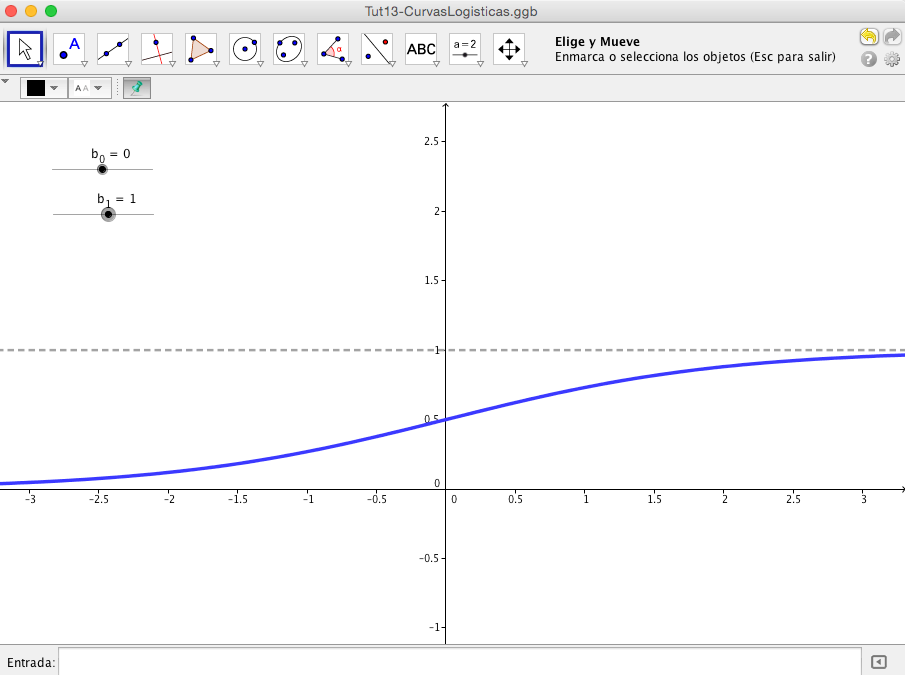
\includegraphics[width=14cm]{../fig/Tut13-CurvasLogisticasGeoGebra.png}
\end{center}
Usa un rato los deslizadores hasta convencerte de que has comprendido el significado de ambos coeficientes.

\section{Estimando los parámetros.}
\label{tut13:sec:EstimandoParametros}

En esta sección vamos a aprender a usar el ordenador para obtener estimaciones de los parámetros $b_0$ y $b_1$, como hemos visto en la Sección \ref{curso-cap13:sec:EstimacionParametros} (pág. \pageref{curso-cap13:sec:EstimacionParametros}) del libro.

\subsection{Valores de $b_0$ y $b_1$  mediante mínimos cuadrados.}
\textcolor{red}{\bf\sc ADVERTENCIA:} Aunque lo hemos avisado en el libro, insistimos. El método que vamos a mostrar aquí {\bf NO} es el que se usa en regresión logística y sólo lo incluimos para que el lector tenga ocasión de darse cuenta de que la regresión logística usa un método distinto del que hemos visto en la regresión lineal simple.

Vamos a ver paso a paso como usar el método de mínimos cuadrados para obtener una curva de la familia logística que aproxime a los datos. Los pasos son los mismos que hemos descrito en la Sección \ref{curso-cap13:subsection:ParametrosCurvaSigmoideaMedianteMinimosCuadrados} (pág. \pageref{curso-cap13:subsection:ParametrosCurvaSigmoideaMedianteMinimosCuadrados}) del libro.

\begin{enumerate}
  \item Aplicar la transformación logit a los valores $\hat p_1,\ldots,\hat p_k$. Llamemos $l_1,\ldots,l_k$ a los valores resultantes. Para hacer esto tenemos qu empezar por asegurarnos de que los valores de las probabilidades están comprendidos entre $0$ y $1$, estrictamente. La razón para hacer esto es que la transformación logit causaría problemas con cualquier valor igual a $0$ o igual a $1$ (ver Ejercicio \ref{tut13:ejercicio02}). Lo conseguimos mediante una selección adecuada  de los elementos del vector {\tt probabilidades}:

\begin{knitrout}
\definecolor{shadecolor}{rgb}{0.969, 0.969, 0.969}\color{fgcolor}\begin{kframe}
\begin{alltt}
\hlstd{(probsAcotadas} \hlkwb{=} \hlstd{(probabilidades} \hlopt{<} \hlnum{1}\hlstd{)} \hlopt{&} \hlstd{(probabilidades} \hlopt{>} \hlnum{0}\hlstd{))}
\end{alltt}
\begin{verbatim}
## [-10,-9.5]  (-9.5,-9]  (-9,-8.5]  (-8.5,-8]  (-8,-7.5]  (-7.5,-7] 
##      FALSE      FALSE      FALSE      FALSE      FALSE      FALSE 
##  (-7,-6.5]  (-6.5,-6]  (-6,-5.5]  (-5.5,-5]  (-5,-4.5]  (-4.5,-4] 
##      FALSE      FALSE      FALSE      FALSE      FALSE      FALSE 
##  (-4,-3.5]  (-3.5,-3]  (-3,-2.5]  (-2.5,-2]  (-2,-1.5]  (-1.5,-1] 
##       TRUE      FALSE       TRUE       TRUE       TRUE       TRUE 
##  (-1,-0.5]   (-0.5,0]    (0,0.5]    (0.5,1]    (1,1.5]    (1.5,2] 
##       TRUE       TRUE       TRUE       TRUE       TRUE       TRUE 
##    (2,2.5]    (2.5,3]    (3,3.5]    (3.5,4]    (4,4.5]    (4.5,5] 
##       TRUE       TRUE      FALSE      FALSE      FALSE      FALSE 
##    (5,5.5]    (5.5,6]    (6,6.5]    (6.5,7]    (7,7.5]    (7.5,8] 
##      FALSE      FALSE      FALSE      FALSE      FALSE      FALSE 
##    (8,8.5]    (8.5,9]    (9,9.5]   (9.5,10] 
##      FALSE      FALSE      FALSE      FALSE
\end{verbatim}
\end{kframe}
\end{knitrout}
Como ves, los valores de probabilidades entre 0 y 1, que se concentran en lo que hemos llamado la {\em zona de transición}, son los que reciben el valor lógico {\tt TRUE}. Ahora ya podemos aplicar la transformación {\tt logit}:

\begin{knitrout}
\definecolor{shadecolor}{rgb}{0.969, 0.969, 0.969}\color{fgcolor}\begin{kframe}
\begin{alltt}
\hlstd{probab2Odds} \hlkwb{=} \hlkwd{log}\hlstd{(probabilidades[probsAcotadas]}\hlopt{/}\hlstd{(}\hlnum{1}\hlopt{-}\hlstd{probabilidades[probsAcotadas]))}
\end{alltt}
\end{kframe}
\end{knitrout}

\item Lo que hacemos es obtener un modelo de regresión lineal simple, ajustado por mínimos cuadrados, del vector {\tt probab2Odds} frente a las marcas de clase correspondientes. En el Tutorial10 aprendimos a usar la función {\tt lm} de R para calcular los coeficientes $\widetilde b_0$ y $\widetilde b_1$ de la recta de regresión
\[l = \widetilde b_0 +\widetilde b_1\cdot w\]

\begin{knitrout}
\definecolor{shadecolor}{rgb}{0.969, 0.969, 0.969}\color{fgcolor}\begin{kframe}
\begin{alltt}
\hlstd{(Oddslm} \hlkwb{=} \hlkwd{lm}\hlstd{(probab2Odds} \hlopt{~} \hlstd{marcasClase[probsAcotadas]))}
\end{alltt}
\begin{verbatim}
## 
## Call:
## lm(formula = probab2Odds ~ marcasClase[probsAcotadas])
## 
## Coefficients:
##                (Intercept)  marcasClase[probsAcotadas]  
##                      0.177                       0.974
\end{verbatim}
\end{kframe}
\end{knitrout}

para los puntos
\[(w_1,l_1),\ldots,(w_k,l_k).\]
Hemos llamado $\widetilde b_0$ y $\widetilde b_1$ a los coeficientes porque, insistimos, el método que estamos exponiendo {\bf no} es el método que aplicaremos en la regresión logística. Y queremos usar símbolos distintos para los valores obtenidos por casa método.

\item Construimos la curva logística correspondiente a esos valores $\widetilde b_0$ y $\widetilde b_1$. Esa curva es, desde luego,
\[
  w = \dfrac{e^{\widetilde{b_0} + \widetilde{b_1} v}}{1 + e^{\widetilde{b_0} + \widetilde{b_1} v}}.
\]
Para obtenerla en R podemos definir una función así:

\begin{knitrout}
\definecolor{shadecolor}{rgb}{0.969, 0.969, 0.969}\color{fgcolor}\begin{kframe}
\begin{alltt}
\hlstd{curvaLogisticaMinCuad} \hlkwb{=} \hlkwa{function}\hlstd{(}\hlkwc{x}\hlstd{)\{}
  \hlstd{b0} \hlkwb{=} \hlstd{Oddslm}\hlopt{$}\hlstd{coefficients[}\hlnum{1}\hlstd{]}
  \hlstd{b1} \hlkwb{=} \hlstd{Oddslm}\hlopt{$}\hlstd{coefficients[}\hlnum{2}\hlstd{]}
  \hlkwd{return}\hlstd{(}\hlkwd{exp}\hlstd{(b0} \hlopt{+} \hlstd{b1} \hlopt{*} \hlstd{x)}\hlopt{/}\hlstd{(}\hlnum{1} \hlopt{+} \hlkwd{exp}\hlstd{(b0} \hlopt{+} \hlstd{b1} \hlopt{*} \hlstd{x)))}
\hlstd{\}}
\end{alltt}
\end{kframe}
\end{knitrout}

que añadimos al gráfico de dispersión con este comando (fíjate en las opciones {\tt add=TRUE} para añadir la curva al gráfico preexistentey \verb#lty="dotted"# para dibujar una curva discontinua):

\begin{knitrout}
\definecolor{shadecolor}{rgb}{0.969, 0.969, 0.969}\color{fgcolor}\begin{kframe}
\begin{alltt}
\hlkwd{points}\hlstd{(marcasClase, probabilidades,} \hlkwc{col}\hlstd{=}\hlstr{"red"}\hlstd{,} \hlkwc{pch}\hlstd{=}\hlnum{2}\hlstd{,} \hlkwc{lwd}\hlstd{=}\hlnum{2}\hlstd{)}
\hlkwd{curve}\hlstd{(curvaLogisticaMinCuad,} \hlkwc{from} \hlstd{=} \hlopt{-}\hlnum{10}\hlstd{,} \hlkwc{to} \hlstd{=} \hlnum{10}\hlstd{,}
      \hlkwc{col}\hlstd{=}\hlstr{"blue"}\hlstd{,} \hlkwc{lwd}\hlstd{=}\hlstr{"2"}\hlstd{,} \hlkwc{add}\hlstd{=}\hlnum{TRUE}\hlstd{,} \hlkwc{lty}\hlstd{=}\hlstr{"dotted"}\hlstd{)}
\end{alltt}
\end{kframe}

{\centering \includegraphics[width=\maxwidth]{figure/pintarCurvaLogisticaMinCuad-1} 

}



\end{knitrout}

\end{enumerate}

Con esto hemos concluido la construcción de este modelo para estimar las probabilidades que, insistimos una vez más, {\bf NO} es el que se usa en regresión logística. En la siguiente sección construiremos finalmente el modelo de regresión logística. Cerramos esta sección con un ejercicio para ayudarte a reflexionar sobre las características del método que hemos descrito.

\begin{ejercicio}
\label{tut13:ejercicio04}
¿Qué sucede  si agrupamos los valores de otra manaera? Cambia el número de clases y comprueba qué sucede con los valores estimados $\widetilde b_0$ y $\widetilde b_1$.
%Soluciones en la página \pageref{tut13:ejercicio04:sol}.
\qed
\end{ejercicio}


\section{Regresión logística:  $b_0$ y $b_1$  mediante maxima verosimilitud.}
\label{tut13:section:ParametrosCurvaSigmoideaMedianteMaximaVerosimilitud}

En esta sección vamos a ver cómo usar el ordenador para obtener las estimaciones de los coeficientesde la curva logística usando el método de máxima verosimilitud, tal como se describe en la Sección \ref{curso-cap13:subsection:ParametrosCurvaSigmoideaMedianteMaximaVerosimilitud} del libro (pág. \pageref{curso-cap13:subsection:ParametrosCurvaSigmoideaMedianteMaximaVerosimilitud}). Primero aprenderemos cómo usar la función {\tt glm} de R y luego, en un apartado opcional, veremos un método más detallado, que puede resultar interesante para quienes quieran adentrarse un poco más en las matemáticas subyacentes al método.

\subsection{La función {\tt glm} de R.}
\label{tut13:subsec:funcionGlm}

En el Tutorial10 conocimos la función {\tt lm} de R, que nos permitía obtener rápida y cómodamente la información relativa a  un modelo de regresión lineal simple. La función {\tt glm} (del inglés, {\em generalized linear model}) juega un papel parecido con respecto a los modelos lineales generalizados, de los que la regresión logística es un ejemplo. Por ejemplo, para obtener los coeficientes del modelo logístico para los datos del Ejemplo \ref{curso-cap13:ejem:EstimacionModeloLogisticoMedianteClases} del libro (pág. \pageref{curso-cap13:ejem:EstimacionModeloLogisticoMedianteClases}), con el que hemos venido trabajando en los apartados anteriores, usaríamos la función {\tt glm} de esta manera:

\begin{knitrout}
\definecolor{shadecolor}{rgb}{0.969, 0.969, 0.969}\color{fgcolor}\begin{kframe}
\begin{alltt}
\hlstd{(glmXY} \hlkwb{=} \hlkwd{glm}\hlstd{(Y} \hlopt{~} \hlstd{X,} \hlkwc{family} \hlstd{=} \hlkwd{binomial}\hlstd{(}\hlkwc{link} \hlstd{=} \hlstr{"logit"}\hlstd{),} \hlkwc{data} \hlstd{= datos))}
\end{alltt}
\begin{verbatim}
## 
## Call:  glm(formula = Y ~ X, family = binomial(link = "logit"), data = datos)
## 
## Coefficients:
## (Intercept)            X  
##      0.0953       1.0701  
## 
## Degrees of Freedom: 999 Total (i.e. Null);  998 Residual
## Null Deviance:	    1390 
## Residual Deviance: 306 	AIC: 310
\end{verbatim}
\end{kframe}
\end{knitrout}

Como en los modelos lineales, hemos guardado el resultado de {\tt glm} en una variable para facilitar el acceso posterior al modelo. Antes de seguir adelante aplicamos {\tt summary} a ese modelo:
\begin{knitrout}
\definecolor{shadecolor}{rgb}{0.969, 0.969, 0.969}\color{fgcolor}\begin{kframe}
\begin{alltt}
\hlstd{(summGlmXY} \hlkwb{=} \hlkwd{summary}\hlstd{(glmXY))}
\end{alltt}
\begin{verbatim}
## 
## Call:
## glm(formula = Y ~ X, family = binomial(link = "logit"), data = datos)
## 
## Deviance Residuals: 
##     Min       1Q   Median       3Q      Max  
## -2.4259  -0.0891   0.0073   0.1124   2.7190  
## 
## Coefficients:
##             Estimate Std. Error z value Pr(>|z|)    
## (Intercept)   0.0953     0.1468    0.65     0.52    
## X             1.0701     0.0857   12.49   <2e-16 ***
## ---
## Signif. codes:  0 '***' 0.001 '**' 0.01 '*' 0.05 '.' 0.1 ' ' 1
## 
## (Dispersion parameter for binomial family taken to be 1)
## 
##     Null deviance: 1385.62  on 999  degrees of freedom
## Residual deviance:  306.23  on 998  degrees of freedom
## AIC: 310.2
## 
## Number of Fisher Scoring iterations: 8
\end{verbatim}
\end{kframe}
\end{knitrout}
Vemos que, como también ocurría con {\tt lm}, al aplicar {\tt summary} al modelo se obtiene mucha más información que con la salida original de {\tt glm}.  La columna {\tt Estimate} de la tabla {\tt Coefficients} contiene los valores estimados de los coeficientes de la curva logística. Y puesto que, {\em ahora sí}, se han obtenido por el método de máxima verosimilitud, podemos llamar $\hat b_0$ y $\hat b_1$ a esas estimaciones.  Y los coeficientes estimados son:

\begin{knitrout}
\definecolor{shadecolor}{rgb}{0.969, 0.969, 0.969}\color{fgcolor}\begin{kframe}
\begin{alltt}
\hlstd{(b0glm} \hlkwb{=} \hlstd{summGlmXY}\hlopt{$}\hlstd{coefficients[}\hlnum{1}\hlstd{])}
\end{alltt}
\begin{verbatim}
## [1] 0.095265
\end{verbatim}
\begin{alltt}
\hlstd{(b1glm} \hlkwb{=} \hlstd{summGlmXY}\hlopt{$}\hlstd{coefficients[}\hlnum{2}\hlstd{])}
\end{alltt}
\begin{verbatim}
## [1] 1.0701
\end{verbatim}
\end{kframe}
\end{knitrout}

como hemos dicho en el Ejemplo \ref{curso-cap13:ejem:CurvaLogisticaPorDosMetodos} (pág. \pageref{curso-cap13:ejem:CurvaLogisticaPorDosMetodos}).

Vamos a añadir la curva logística correspondiente a estos coeficientes al diagrama de dispersión. Esa curva aparece en la siguiente figura en trazos (opción \verb#lty="dashed"#) rojos. El código es muy parecido al que hemos usado antes para la curva que obtuvimos usando mínimos cuadrados:

\begin{knitrout}
\definecolor{shadecolor}{rgb}{0.969, 0.969, 0.969}\color{fgcolor}\begin{kframe}
\begin{alltt}
\hlkwd{curve}\hlstd{(curvaLogisticaMinCuad,} \hlkwc{from} \hlstd{=} \hlopt{-}\hlnum{10}\hlstd{,} \hlkwc{to} \hlstd{=} \hlnum{10}\hlstd{,}
      \hlkwc{col}\hlstd{=}\hlstr{"blue"}\hlstd{,} \hlkwc{lwd}\hlstd{=}\hlstr{"2"}\hlstd{,} \hlkwc{add}\hlstd{=}\hlnum{TRUE}\hlstd{,} \hlkwc{lty}\hlstd{=}\hlstr{"dotted"}\hlstd{)}
\hlstd{curvaLogisticaGLM} \hlkwb{=} \hlkwa{function}\hlstd{(}\hlkwc{x}\hlstd{)\{}
  \hlkwd{return}\hlstd{(}\hlkwd{exp}\hlstd{(b0glm} \hlopt{+} \hlstd{b1glm} \hlopt{*} \hlstd{x)}\hlopt{/}\hlstd{(}\hlnum{1} \hlopt{+} \hlkwd{exp}\hlstd{(b0glm} \hlopt{+} \hlstd{b1glm} \hlopt{*} \hlstd{x)))}
\hlstd{\}}
\hlkwd{curve}\hlstd{(curvaLogisticaGLM,} \hlkwc{from} \hlstd{=} \hlopt{-}\hlnum{10}\hlstd{,} \hlkwc{to} \hlstd{=} \hlnum{10}\hlstd{,}
      \hlkwc{col}\hlstd{=}\hlstr{"red"}\hlstd{,} \hlkwc{lwd}\hlstd{=}\hlstr{"2"}\hlstd{,} \hlkwc{add}\hlstd{=}\hlnum{TRUE}\hlstd{,} \hlkwc{lty}\hlstd{=}\hlstr{"dashed"}\hlstd{)}
\hlkwd{legend}\hlstd{(}\hlkwc{x}\hlstd{=}\hlstr{"right"}\hlstd{,} \hlkwc{legend}\hlstd{=}\hlkwd{c}\hlstd{(}\hlstr{"M<U+00E1>xima verosimilitud"}\hlstd{,} \hlstr{"M<U+00ED>nimos cuadrados"}\hlstd{),}
       \hlkwc{col} \hlstd{=} \hlkwd{c}\hlstd{(}\hlstr{"red"}\hlstd{,} \hlstr{"blue"}\hlstd{),} \hlkwc{bty}\hlstd{=}\hlnum{1}\hlstd{,} \hlkwc{lty}\hlstd{=}\hlkwd{c}\hlstd{(}\hlstr{"dashed"}\hlstd{,}\hlstr{"dotted"}\hlstd{),}\hlkwc{lwd}\hlstd{=}\hlnum{3}\hlstd{,}\hlkwc{cex}\hlstd{=}\hlnum{1.5}\hlstd{)}
\end{alltt}
\end{kframe}

{\centering \includegraphics[width=\maxwidth]{figure/pintarCurvaLogisticasDosModelos-1} 

}



\end{knitrout}




La figura que hemos obtenido es, esencialmente, la Figura \ref{curso-cap13:fig:CurvaLogisticaPorDosMetodos} del libro (pág. \pageref{curso-cap13:fig:CurvaLogisticaPorDosMetodos}).

Volviendo a los resultados de {\tt glm}, el lector habrá observado sin duda la gran cantidad de información que hemos obtenido. Hay una parte de esa información que va más allá de lo que nosotros vamos a aprender en este curso. Pero en el Capítulo \ref{curso-cap:RegresionLogistica} y en las siguientes seccione de este tutorial vamos a tratar de llegar tan lejos como nos sea posible en el análisis de esa información.

Para cerrar este apartado, recuerda que los coeficientes $\hat b_0$ y $\hat b_1$ que hemos obtenido con {\tt glm} son, aproximadamente, los que producen un valor máximo de la función verosimilitud (no corresponden exactamente al máximo porque se han obtenido por un método numérico). ¿Y cuál es ese valor máximo de la verosimilitud? En R es muy fácil obtenerlo a partir del modelo. De hecho, lo que es inmediato es obtener el logaritmo de la verosimilitud:
\begin{knitrout}
\definecolor{shadecolor}{rgb}{0.969, 0.969, 0.969}\color{fgcolor}\begin{kframe}
\begin{alltt}
\hlstd{(logVerosimilitud} \hlkwb{=} \hlkwd{logLik}\hlstd{(glmXY))}
\end{alltt}
\begin{verbatim}
## 'log Lik.' -153.11 (df=2)
\end{verbatim}
\end{kframe}
\end{knitrout}
El resultado incluye varias {\em decoraciones:} un nombre e información sobre los grados de libertad del modelo (hablaremos de esto más adelante). Para eliminar esa información extra y acceder simplemente al valor del logaritmo de la verosimilitud hacemos un pequeño cambio:
\begin{knitrout}
\definecolor{shadecolor}{rgb}{0.969, 0.969, 0.969}\color{fgcolor}\begin{kframe}
\begin{alltt}
\hlstd{(logVerosimilitud} \hlkwb{=} \hlkwd{logLik}\hlstd{(glmXY)[}\hlnum{1}\hlstd{])}
\end{alltt}
\begin{verbatim}
## [1] -153.11
\end{verbatim}
\end{kframe}
\end{knitrout}

Y ahora la versosimilitud es simplemente:
\begin{knitrout}
\definecolor{shadecolor}{rgb}{0.969, 0.969, 0.969}\color{fgcolor}\begin{kframe}
\begin{alltt}
\hlstd{(verosimilitud} \hlkwb{=} \hlkwd{exp}\hlstd{(logVerosimilitud))}
\end{alltt}
\begin{verbatim}
## [1] 3.1899e-67
\end{verbatim}
\end{kframe}
\end{knitrout}

Por el momento este resultado no parece de mucha utilidad. Al fin y al cabo, lo que nos trajo aquí era el deseo de estimar los coeficientes de la curva logística, mientras que la verosimilitud parecía sólo una herramienta para hacer esa estimación. Pero cuando lleguemos a los apartados sobre inferencia en la regresión logística veremos que este valor de la verosimilitud juega un papel importante.


\begin{ejercicio}
\label{tut13:ejercicio05}

\begin{enumerate}
\item[]

\item Comprueba los valores de $b_0$ y $b_1$ que aparecen en el Ejemplo \ref{curso-cap13:ejem:coeficientesLogisticaVasculopatia} del libro (pág. \pageref{curso-cap13:ejem:coeficientesLogisticaVasculopatia}) para el modelo que relaciona itb y vasculopatía.

\item Añade la curva logística al diagrama  de dispersión de esos datos y compara con la Figura \ref{curso-cap13:fig:CurvaLogisticaVasculopatia} del libro (pág. \pageref{curso-cap13:fig:CurvaLogisticaVasculopatia}).

\item Calcula la verosimilitud de ese modelo logístico.

\end{enumerate}

%Soluciones en la página \pageref{tut13:ejercicio05:sol}.
\qed
\end{ejercicio}


\subsection{Predicción con el modelo logístico.}
\label{tut13:subsec:PrediccionConModeloLogistico}

Desde que introdujimos la idea de modelo en esta parte del curso hemos insistido en varias ocasiones en que una de las finalidades básicas de los modelos son las predicciones. En el caso del modelo de regresión logística las primeras predicciones que podemos obtener del modelo son los {\em valores ajustados} correspondientes  a los datos de la variable explicativa $X$ que hemos usado para construir el modelo. Es decir, que para cada punto $(x_i, y_i)$ de la muestra obtenemos un valor predicho de la probabilidad:
\[\hat\pi(x)=\dfrac{e^{b_0+b_1\cdot x}}{1+e^{b_0+b_1\cdot x}}.\]
Después de usar {\tt glm}, esos valores ajustados de las probabilidades están almacenados en un vector de R que es la componente {\tt fitted.values} del modelo. En el ejemplo con el que estamos trabajando, podemos explorar esas predicciones así:

\begin{knitrout}
\definecolor{shadecolor}{rgb}{0.969, 0.969, 0.969}\color{fgcolor}\begin{kframe}
\begin{alltt}
\hlkwd{head}\hlstd{(glmXY}\hlopt{$}\hlstd{fitted.values)}
\end{alltt}
\begin{verbatim}
##          1          2          3          4          5          6 
## 0.01792953 0.04952345 0.00139781 0.99990542 0.00018127 0.00559471
\end{verbatim}
\begin{alltt}
\hlkwd{tail}\hlstd{(glmXY}\hlopt{$}\hlstd{fitted.values)}
\end{alltt}
\begin{verbatim}
##         995         996         997         998         999        1000 
## 0.000053528 0.999308273 0.274343833 0.999971163 0.002542159 0.362394478
\end{verbatim}
\end{kframe}
\end{knitrout}

En este ejemplo, con una muestra de $n = 1000$ puntos, al representar gráficamente esas predicciones el resultado cubre casi completamente la curva logística que produce el modelo. Para facilitar la visualización hemos pintado la curva logística con un trazo gris grueso, y en su interior puedes ver, en negro, las probabilidades que predice el modelo para cada valor de $X$:

\begin{knitrout}
\definecolor{shadecolor}{rgb}{0.969, 0.969, 0.969}\color{fgcolor}\begin{kframe}
\begin{verbatim}
## [1] 0.095265
## [1] 1.0701
\end{verbatim}
\end{kframe}

{\centering \includegraphics[width=\maxwidth]{figure/dibujarCurvaLogistica-1} 

}



\end{knitrout}

En el Tutorial10, al estudiar el modelo de regresión lineal, también vimos que se podía usar la función {\tt predict} para obtener predicciones del modelo para valores
de $X$ fuera de la muestra. Por ejemplo, para $x=3$ haríamos:

\begin{knitrout}
\definecolor{shadecolor}{rgb}{0.969, 0.969, 0.969}\color{fgcolor}\begin{kframe}
\begin{alltt}
\hlstd{x0} \hlkwb{=} \hlnum{3}
\hlkwd{predict}\hlstd{(glmXY,} \hlkwc{newdata} \hlstd{=} \hlkwd{data.frame}\hlstd{(}\hlkwc{X}\hlstd{=x0))}
\end{alltt}
\begin{verbatim}
##      1 
## 3.3056
\end{verbatim}
\end{kframe}
\end{knitrout}

Pero el valor es mayor que 1... ¿no estábamos prediciendo probabilidades? La respuesta es que, por defecto, lo que devuelve {\tt predict} es el valor del término $b_0 + b_1 x$ para el modelo. Vamos a comprobarlo:

\begin{knitrout}
\definecolor{shadecolor}{rgb}{0.969, 0.969, 0.969}\color{fgcolor}\begin{kframe}
\begin{alltt}
\hlstd{b0glm} \hlopt{+} \hlstd{b1glm} \hlopt{*} \hlstd{x0}
\end{alltt}
\begin{verbatim}
## [1] 3.3056
\end{verbatim}
\end{kframe}
\end{knitrout}

¿Y si lo que queremos es la predicción de la probabilidad? En ese caso usamos el argumento opcional \verb#type = "response"# de {\tt predict}

\begin{knitrout}
\definecolor{shadecolor}{rgb}{0.969, 0.969, 0.969}\color{fgcolor}\begin{kframe}
\begin{alltt}
\hlkwd{predict}\hlstd{(glmXY,} \hlkwc{newdata} \hlstd{=} \hlkwd{data.frame}\hlstd{(}\hlkwc{X}\hlstd{=x0),} \hlkwc{type} \hlstd{=} \hlstr{"response"}\hlstd{)}
\end{alltt}
\begin{verbatim}
##       1 
## 0.96462
\end{verbatim}
\end{kframe}
\end{knitrout}

El valor por defecto es \verb#type = "link"#  y ya hemos visto que produce como resultado predicciones en la escala del término lineal $b_0 + b_1 x$. El valor de la probabilidad que hemos obtenido es, desde luego, el mismo que obtendríamos sustituyendo el valor de $X$ en la curva logística del modelo:

\begin{knitrout}
\definecolor{shadecolor}{rgb}{0.969, 0.969, 0.969}\color{fgcolor}\begin{kframe}
\begin{alltt}
\hlkwd{exp}\hlstd{(b0glm} \hlopt{+} \hlstd{b1glm} \hlopt{*} \hlstd{x0)} \hlopt{/} \hlstd{(}\hlnum{1} \hlopt{+} \hlkwd{exp}\hlstd{(b0glm} \hlopt{+} \hlstd{b1glm} \hlopt{*} \hlstd{x0))}
\end{alltt}
\begin{verbatim}
## [1] 0.96462
\end{verbatim}
\end{kframe}
\end{knitrout}

Y, finalmente, también podemos obtener ese valor usando la función {\tt plogis}, de la que aún no hemos hablado:

\begin{knitrout}
\definecolor{shadecolor}{rgb}{0.969, 0.969, 0.969}\color{fgcolor}\begin{kframe}
\begin{alltt}
\hlkwd{plogis}\hlstd{(b0glm} \hlopt{+} \hlstd{b1glm} \hlopt{*} \hlstd{x0)}
\end{alltt}
\begin{verbatim}
## [1] 0.96462
\end{verbatim}
\end{kframe}
\end{knitrout}
No vamos a entrar en muchos más detalles sobre {\tt plogis} (el lector interesado puede consultar la ayuda). Nos limitaremos a explicar que el valor de {\tt plogis(u)}, para un número $u$, es
\[\mbox{\tt plogis(u)} = \dfrac{e^u}{1 + e^u}\]


\subsection{Cálculo directo del modelo a partir de la función verosimilitud.}
\label{tut13:subsec:calculoDirectoFuncionVerosimilitud}
\noindent{\bf Opcional: esta sección puede omitirse en una primera lectura.}\\

En este apartado, en lugar de recurrir a la función {\tt glm} de R, vamos a construir explícitamente la función verosimilitud y vamos a buscar su valor máximo de otra manera. Recuerda que en la Ecuación \ref{curso-cap13:ecu:FuncionVerosimilitudLogistica} del libro (pág. \ref{curso-cap13:ecu:FuncionVerosimilitudLogistica}) hemos visto que la función verosimilitud se puede expresar así:

\[
{\cal L}(x_1,x_2,\ldots,x_n, y_1, y_2, \ldots, y_n;b_0, b_1) =\prod_{i:y_i=1}\hat{\pi}(x_i)  \cdot \prod_{i:y_i=0}(1 - \hat{\pi}(x_i))
\]
\[
=\prod_{i:y_i=1} \dfrac{e^{b_0+b_1\cdot x_i}}{1+e^{b_0+b_1\cdot x_i}}
\cdot \prod_{i:y_i=0}\dfrac{1}{1+e^{b_0+b_1\cdot x_i}}
\]

Vamos a empezar por traducir esta expresión a R. Recuerda que aquí pensamos en $b_0, b_1$ como variables, mientras que $X$ e $Y$ son parámetros.

\begin{knitrout}
\definecolor{shadecolor}{rgb}{0.969, 0.969, 0.969}\color{fgcolor}\begin{kframe}
\begin{alltt}
\hlstd{verosimilitud} \hlkwb{=} \hlkwa{function}\hlstd{(}\hlkwc{b}\hlstd{)\{}
    \hlkwd{prod}\hlstd{(}\hlkwd{exp}\hlstd{(b[}\hlnum{1}\hlstd{]} \hlopt{+} \hlstd{b[}\hlnum{2}\hlstd{]} \hlopt{*} \hlstd{X[Y}\hlopt{==}\hlnum{1}\hlstd{])} \hlopt{/}\hlstd{(}\hlnum{1} \hlopt{+} \hlkwd{exp}\hlstd{(b[}\hlnum{1}\hlstd{]} \hlopt{+} \hlstd{b[}\hlnum{2}\hlstd{]} \hlopt{*} \hlstd{X[Y}\hlopt{==}\hlnum{1}\hlstd{])))} \hlopt{*}
    \hlkwd{prod}\hlstd{(}\hlnum{1} \hlopt{/}\hlstd{(}\hlnum{1} \hlopt{+} \hlkwd{exp}\hlstd{(b[}\hlnum{1}\hlstd{]} \hlopt{+} \hlstd{b[}\hlnum{2}\hlstd{]} \hlopt{*} \hlstd{X[Y}\hlopt{==}\hlnum{0}\hlstd{])))}
\hlstd{\}}
\end{alltt}
\end{kframe}
\end{knitrout}

A continuación vamos a representar gráficamente esta función verosimilitud. Puesto que es una función de dos variables, su gráfica es una superficie en el espacio tridimensional. Ya hemos encontrado alguna de estas gráficas en otros tutoriales. Y no nos vamos a extender mucho sobre los comandos de R que vamos a utilizar. Los mostraremos simplemente para que el lector interesado sepa por dónde empezar a buscar si en el futuro necesita profundizar en esto:

\begin{knitrout}
\definecolor{shadecolor}{rgb}{0.969, 0.969, 0.969}\color{fgcolor}\begin{kframe}
\begin{alltt}
\hlcom{# Creamos una malla o reticula de valores de b0, b1 en los que}
\hlcom{# evaluaremos la funcion verosimilitud mediante la funcion outer}
\hlstd{valores_b0} \hlkwb{=} \hlkwd{seq}\hlstd{(}\hlopt{-}\hlnum{0.5}\hlstd{,} \hlnum{0.5}\hlstd{,} \hlkwc{length.out} \hlstd{=} \hlnum{50}\hlstd{)}\hlcom{#seq(25, 35, length.out = 60)}
\hlstd{valores_b1} \hlkwb{=} \hlkwd{seq}\hlstd{(}\hlnum{0.7}\hlstd{,} \hlnum{1.5}\hlstd{,} \hlkwc{length.out} \hlstd{=} \hlnum{50}\hlstd{)}\hlcom{#seq(-38, -28, length.out = 60)}

\hlcom{# Para la representacion que vamos a hacer necesitamos vectorializar}
\hlcom{# la funcion verosimilitud.}
\hlstd{verosimilitud_vect} \hlkwb{=} \hlkwd{Vectorize}\hlstd{(}\hlkwa{function}\hlstd{(}\hlkwc{b0}\hlstd{,} \hlkwc{b1}\hlstd{)}\hlkwd{verosimilitud}\hlstd{(}\hlkwd{c}\hlstd{(b0, b1)))}

\hlcom{# Usando outer calculamos la verosimilitud para cada}
\hlcom{# combinacion de b0 y b1 en la malla que hemos creado}
\hlstd{zp} \hlkwb{=} \hlkwd{outer}\hlstd{(valores_b0, valores_b1, verosimilitud_vect)}

\hlcom{# Y finalmente persp se encarga de crear el grafico tridimensional}
\hlkwd{persp}\hlstd{(valores_b0, valores_b1, zp,}
      \hlkwc{theta}\hlstd{=}\hlnum{45}\hlstd{,} \hlkwc{phi}\hlstd{=}\hlnum{20}\hlstd{,} \hlcom{# angulos de visualizacion}
      \hlkwc{col}\hlstd{=}\hlstr{"lightblue"}\hlstd{,} \hlkwc{xlab}\hlstd{=}\hlstr{"b0"}\hlstd{,} \hlkwc{ylab}\hlstd{=}\hlstr{"b1"}\hlstd{,} \hlkwc{zlab}\hlstd{=}\hlstr{"Verosimilitud"}\hlstd{)}
\end{alltt}
\end{kframe}

{\centering \includegraphics[width=\maxwidth]{figure/graficaVerosimilitud-1} 

}



\end{knitrout}

La figura que hemos obtenido deja claro que la verosimilitud es máxima para los valores de $b_0$ y $b_1$ que proporciona el método. En el anterior apartado hemos obtenido esos valores usando {\tt glm}. Pero el problema de encontrar valores mínimos (o máximos) de una función es un problema muy general y que se presenta muy a menudo en una colección muy variada de situaciones. No es de extrañar, por tanto, que exista una parte de las matemáticas dedicada precisamente a eso. La {\sf Optimización} estudia los métodos para localizar esos valores extremos (máximos o mínimos) de una función bajo una serie de condiciones. En R disponemos de varias herramientas de optimización que en muchas ocasiones son suficientes. Una de esas herramientas es la función {\tt optim}. No podemos extendernos demasiado sobre esta herramienta, porque las posibilidades de configurarla son muy amplias. Nosotros vamos a usar uno de los métodos de optimización disponibles, concretamente el método llamado {\sf BFGS} por sus autores, (Broyden, Fletcher, Goldfarb, Shanno). El lector interesado puede encontrar más información en la ayuda de la función {\tt optim} o en el libro (más información usando el enlace)
\begin{center}
\link{https://www.crcpress.com/product/isbn/9781439884485}{{\em Using R for Numerical Analysis in Science and Engineering} de V. Bloomfield}
\end{center}

Para usar ese método debemos proporcionarle a la función {\tt optim} un método para calcular los valores del {\sf gradiente} de la verosimilitud. El gradiente es el vector formado por las dos derivadas parciales:
\[
\operatorname{grad}({\cal L}) = \left(
\dfrac{\partial {\cal L}}{\partial b_0}, \dfrac{\partial {\cal L}}{\partial b_1}
\right)
\]

La función verosimilitud es, como hemos visto, muy complicada. Vamos a simplificar las cosas un poco considerando el logaritmo con signo negativo de la verosimilitud El signo se debe a que {\tt optim}, como la mayoría de las funciones de optimización, localiza siempre los valores {\em mínimos} de la función. Además, en lugar de tratar de encontrar una fórmula para el gradiente, la librería {\tt pracma} de R contiene una función {\tt grad} que permite estimar los valores del gradiente de una función. Así que usaremos esa función para proporcionarle a {\tt optim} los valores del gradiente que requiere el método {\sf BFGS}. Recuerda instalar la llibrería {\tt pracma} antes de usarla:

\begin{knitrout}
\definecolor{shadecolor}{rgb}{0.969, 0.969, 0.969}\color{fgcolor}\begin{kframe}
\begin{alltt}
\hlkwd{library}\hlstd{(pracma)}

\hlcom{# Definimos el logaritmo con signo negativo de la funcion verosimilitud}
\hlstd{logVerosmltd} \hlkwb{=} \hlkwa{function}\hlstd{(}\hlkwc{b}\hlstd{)\{}
  \hlopt{-} \hlkwd{log}\hlstd{(}\hlkwd{verosimilitud}\hlstd{(b))}
\hlstd{\}}

\hlcom{# Y usamos grad para estimar su gradiente en un punto b = (b0, b1)}
\hlstd{grad_logVerosmltd} \hlkwb{=} \hlkwa{function}\hlstd{(}\hlkwc{b}\hlstd{)\{}\hlkwd{grad}\hlstd{(logVerosmltd,} \hlkwc{x0} \hlstd{= b)\}}
\end{alltt}
\end{kframe}
\end{knitrout}

Ahora ya estamos listos para usar la función {\tt optim}. Para hacerlo debemos darle un valor inicial aproximado de $b_0$ y $b_1$. Como, en principio, no tenemos ninguna estimación, simplemente tomaremos ambos iguales a $1$. Al tratarse de un método aproximado, otros valores iniciales producirían resultados ligeramente distintos. Puedes experimentar con otros valores. El resultado de {\tt optim} contiene bastante información sobre el proceso de optimización asociado al método {\sf BFGS}:

{\small
\begin{knitrout}
\definecolor{shadecolor}{rgb}{0.969, 0.969, 0.969}\color{fgcolor}\begin{kframe}
\begin{alltt}
\hlstd{(optimizacion} \hlkwb{=}
   \hlkwd{optim}\hlstd{(}\hlkwc{par} \hlstd{=} \hlkwd{c}\hlstd{(}\hlnum{1}\hlstd{,} \hlnum{1}\hlstd{),} \hlkwc{fn} \hlstd{= logVerosmltd,} \hlkwc{gr} \hlstd{= grad_logVerosmltd,} \hlkwc{method}\hlstd{=}\hlstr{"BFGS"}\hlstd{))}
\end{alltt}
\begin{verbatim}
## $par
## [1] 0.095265 1.070099
## 
## $value
## [1] 153.11
## 
## $counts
## function gradient 
##       30        9 
## 
## $convergence
## [1] 0
## 
## $message
## NULL
\end{verbatim}
\end{kframe}
\end{knitrout}
}

La componente {\tt par} del resultado contiene la estimación de los valores $b_0$ y $b_1$ que producen el resultado óptimo:
\begin{knitrout}
\definecolor{shadecolor}{rgb}{0.969, 0.969, 0.969}\color{fgcolor}\begin{kframe}
\begin{alltt}
\hlstd{optimizacion}\hlopt{$}\hlstd{par}
\end{alltt}
\begin{verbatim}
## [1] 0.095265 1.070099
\end{verbatim}
\end{kframe}
\end{knitrout}
y si comparas con lo que obtuvimos en la sección previa usando {\tt glm} verás que son los mismos valores:
\begin{knitrout}
\definecolor{shadecolor}{rgb}{0.969, 0.969, 0.969}\color{fgcolor}\begin{kframe}
\begin{alltt}
\hlstd{summGlmXY}\hlopt{$}\hlstd{coefficients}
\end{alltt}
\begin{verbatim}
##             Estimate Std. Error  z value   Pr(>|z|)
## (Intercept) 0.095265    0.14684  0.64877 5.1649e-01
## X           1.070099    0.08567 12.49100 8.3591e-36
\end{verbatim}
\end{kframe}
\end{knitrout}
Insistimos, en cualquier caso, en que los resultados dependen de los valores iniciales de $b_i$ que hemos usado en {\tt optim}. Otros valores podrían producir unas estimaciones menos parecidas a las de {\tt glm}.

\begin{ejercicio}
\label{tut13:ejercicio06}
La componente {\tt value} del resultado de {\tt optim}, que es 153.11, también tiene una interpretación relacionada con los resultados que obtuvimos con {\tt glm}. ¿Cuál es esa interpretación?
%Soluciones en la página \pageref{tut13:ejercicio06:sol}.
\qed
\end{ejercicio}


\section{Inferencia en regresi\'on log\'istica.}
\label{tut13:sec:inferencia}

\subsection{El estadístico de Wald.}

En la Ecuación \ref{curso-cap13:ecu:EstadisticoWaldRegresionLogistica} del libro (pág. \pageref{curso-cap13:ecu:EstadisticoWaldRegresionLogistica}) hemos visto el {\sf Estadístico de Wald} para el coeficiente $\beta_1$ del modelo de regresión logística:
\[
\Xi = \dfrac{b_1}{SE(b_1)}
\]
Dijimos entonces que no íbamos a dar una expresión explícita del error estándar $SE(b_1)$, porque usaríamos el ordenador para obtener el valor de ese error. Vamos a empezar esta sección señalando que la función {\tt glm} de R ya nos ha proporcionado ese resultado. En efecto, si recordamos la tabla de coeficientes

\begin{knitrout}
\definecolor{shadecolor}{rgb}{0.969, 0.969, 0.969}\color{fgcolor}\begin{kframe}
\begin{alltt}
\hlstd{summGlmXY}\hlopt{$}\hlstd{coefficients}
\end{alltt}
\begin{verbatim}
##             Estimate Std. Error  z value   Pr(>|z|)
## (Intercept) 0.095265    0.14684  0.64877 5.1649e-01
## X           1.070099    0.08567 12.49100 8.3591e-36
\end{verbatim}
\end{kframe}
\end{knitrout}

vemos que el título de la segunda columna es precisamente {\tt Std. Error}, ya que los elementos de esa clumna son los errores estándar de los estadísticos de Wald correspondientes, respectivamente, a $\beta_0$ (en la fila {\tt Intercept}) y $\beta_1$ (en la fila con el nombre {\tt X} de la variable predictora). En particular el valor de $SE(b_1)$ es, entonces:

\begin{knitrout}
\definecolor{shadecolor}{rgb}{0.969, 0.969, 0.969}\color{fgcolor}\begin{kframe}
\begin{alltt}
\hlstd{summGlmXY}\hlopt{$}\hlstd{coefficients[}\hlnum{2}\hlstd{,} \hlnum{2}\hlstd{]}
\end{alltt}
\begin{verbatim}
## [1] 0.08567
\end{verbatim}
\end{kframe}
\end{knitrout}

Por lo tanto el estadístico de Wald es:

\begin{knitrout}
\definecolor{shadecolor}{rgb}{0.969, 0.969, 0.969}\color{fgcolor}\begin{kframe}
\begin{alltt}
\hlstd{(WaldBeta1} \hlkwb{=} \hlstd{summGlmXY}\hlopt{$}\hlstd{coefficients[}\hlnum{2}\hlstd{,} \hlnum{1}\hlstd{]} \hlopt{/} \hlstd{summGlmXY}\hlopt{$}\hlstd{coefficients[}\hlnum{2}\hlstd{,} \hlnum{2}\hlstd{])}
\end{alltt}
\begin{verbatim}
## [1] 12.491
\end{verbatim}
\end{kframe}
\end{knitrout}

Puedes comprobar que el valor del estadístico es precisamente el que aparece en la tercera columna de la tabla, titulada {\tt z value}. Y la razón de ese título es que, como hemos visto en el libro, $\Xi$ se distribuye como una normal estándar $Z$. También hemos dicho que actualmente no se considera adecuado usar este estadístico de Wald $\Xi$ para hacer contrastes de hipótesis sobre $\beta_1$, por las razones que hemos expuesto en el libro. Pero por si alguna vez necesitras hacerlo, el p-valor se calcularía como en un contraste bilateral con $Z$ (fíjate en que usamos la cola derecha):

\begin{knitrout}
\definecolor{shadecolor}{rgb}{0.969, 0.969, 0.969}\color{fgcolor}\begin{kframe}
\begin{alltt}
\hlstd{(pValorWald} \hlkwb{=} \hlnum{2} \hlopt{*} \hlstd{(}\hlkwd{pnorm}\hlstd{(WaldBeta1,} \hlkwc{lower.tail} \hlstd{=} \hlnum{FALSE}\hlstd{)))}
\end{alltt}
\begin{verbatim}
## [1] 8.3591e-36
\end{verbatim}
\end{kframe}
\end{knitrout}
Y ahora ya está claro que la última columna de la tabla contiene los p-valores de los contrastes para $\beta_0$ y $\beta_1$, usando los correspondientes estadísticos de Wald.

\subsubsection{Selección de modelos y devianza.}
\label{cap13:subsubsec:SeleccionModelosDevianza}

En la Ecuación \ref{curso-cap13:ecu:EcuacionGlm} del libro (pág. \pageref{curso-cap13:ecu:EcuacionGlm}) hemos definido la devianza mediante
\[
D(modelo) = - 2\ln({\cal L}(modelo)).
\]
Y sin duda, el lector atento habrá reparado en que uno de los resultados de {\tt glm} es

\begin{knitrout}
\definecolor{shadecolor}{rgb}{0.969, 0.969, 0.969}\color{fgcolor}\begin{kframe}
\begin{alltt}
\hlstd{summGlmXY}\hlopt{$}\hlstd{deviance}
\end{alltt}
\begin{verbatim}
## [1] 306.23
\end{verbatim}
\end{kframe}
\end{knitrout}

Vamos a confirmar que este resultado coincide con la anterior definición. Antes hemos aprendido a calcular el logaritmo de la verosimilitud con {\tt logLik}, así que hacemos:

\begin{knitrout}
\definecolor{shadecolor}{rgb}{0.969, 0.969, 0.969}\color{fgcolor}\begin{kframe}
\begin{alltt}
\hlopt{-} \hlnum{2} \hlopt{*} \hlkwd{logLik}\hlstd{(glmXY)}
\end{alltt}
\begin{verbatim}
## 'log Lik.' 306.23 (df=2)
\end{verbatim}
\end{kframe}
\end{knitrout}

e, ignorando las {\em decoraciones} que R añade, vemos que el valor de la devianza que proporciona {\tt glm} es el esperado.

Pero además, {\tt glm} también nos proporciona la devianza del llamado {\em modelo nulo}, el que se obtiene suponiendo que la hipótesis nula $H_0=\{\beta_1= 0\}$ es cierta:

\begin{knitrout}
\definecolor{shadecolor}{rgb}{0.969, 0.969, 0.969}\color{fgcolor}\begin{kframe}
\begin{alltt}
\hlstd{summGlmXY}\hlopt{$}\hlstd{null.deviance}
\end{alltt}
\begin{verbatim}
## [1] 1385.6
\end{verbatim}
\end{kframe}
\end{knitrout}

Y, por lo tanto, el estadístico $G$ de la Ecuación \ref{curso-cap13:ecu:EstadisticoG} del libro (pág. \pageref{curso-cap13:ecu:EstadisticoG}) es muy fácil de obtener:


\begin{knitrout}
\definecolor{shadecolor}{rgb}{0.969, 0.969, 0.969}\color{fgcolor}\begin{kframe}
\begin{alltt}
\hlstd{(G} \hlkwb{=} \hlstd{summGlmXY}\hlopt{$}\hlstd{null.deviance} \hlopt{-} \hlstd{summGlmXY}\hlopt{$}\hlstd{deviance)}
\end{alltt}
\begin{verbatim}
## [1] 1079.4
\end{verbatim}
\end{kframe}
\end{knitrout}

Y, puesto que sabemos que $G$ tiene una distribución muestral $\chi^2_1$, obtenemos el p-valor del contraste de $H_0$ así:

\begin{knitrout}
\definecolor{shadecolor}{rgb}{0.969, 0.969, 0.969}\color{fgcolor}\begin{kframe}
\begin{alltt}
\hlstd{(pValor} \hlkwb{=} \hlkwd{pchisq}\hlstd{(G,} \hlkwc{lower.tail} \hlstd{=} \hlnum{FALSE}\hlstd{,} \hlkwc{df}\hlstd{=}\hlnum{1}\hlstd{))}
\end{alltt}
\begin{verbatim}
## [1] 9.9536e-237
\end{verbatim}
\end{kframe}
\end{knitrout}

Con un p-valor tan (ridículamente) pequeño, es evidente que la hipótesis nula se rechaza. Eso se interpreta como una evidencia significativa de que el modelo con $\beta_1\neq 0$ explica mejor la relación entre las variables $X$ e $Y$ que el modelo nulo con $\beta_1 = 0$.

\begin{ejercicio}
\label{tut13:ejercicio07}
Comprueba los resultados del Ejemplo \ref{curso-cap13:ejem:contrasteBeta1vasculopatia} del libro (pág. \pageref{curso-cap13:ejem:contrasteBeta1vasculopatia}).
%Soluciones en la página \pageref{tut13:ejercicio07:sol}.
\qed
\end{ejercicio}



\subsubsection{Intervalos de confianza para $\beta_0$ y $\beta_1$}

En la Ecuación \ref{curso-cap13:ecu:IntconfBetaRegresionLogistica} del libro (pág. \pageref{curso-cap13:ecu:IntconfBetaRegresionLogistica}) hemos visto que podemos usar los valores de los errores estándar que intervienen en el Estadístico de Wald para construir intervalos de confianza para $\beta_0$ y $\beta_1$. Y una vez que sabemos que esos errores estándar aparecen en la tabla que hemos obtenido de {\tt glm}, la construcción de dichos intervalos es muy sencilla:

\begin{knitrout}
\definecolor{shadecolor}{rgb}{0.969, 0.969, 0.969}\color{fgcolor}\begin{kframe}
\begin{alltt}
\hlstd{nc} \hlkwb{=} \hlnum{0.95}
\hlstd{alfa} \hlkwb{=} \hlnum{1} \hlopt{-} \hlstd{nc}
\hlstd{alfaMedios} \hlkwb{=} \hlstd{alfa}\hlopt{/}\hlnum{2}
\hlstd{zAlfaMedios} \hlkwb{=} \hlkwd{qnorm}\hlstd{(}\hlnum{1} \hlopt{-} \hlstd{alfaMedios)}

\hlstd{(b0} \hlkwb{=} \hlstd{summGlmXY}\hlopt{$}\hlstd{coefficients[}\hlnum{1}\hlstd{,} \hlnum{1}\hlstd{])}
\end{alltt}
\begin{verbatim}
## [1] 0.095265
\end{verbatim}
\begin{alltt}
\hlstd{(b1} \hlkwb{=} \hlstd{summGlmXY}\hlopt{$}\hlstd{coefficients[}\hlnum{2}\hlstd{,} \hlnum{1}\hlstd{])}
\end{alltt}
\begin{verbatim}
## [1] 1.0701
\end{verbatim}
\begin{alltt}
\hlstd{(SE_b0} \hlkwb{=} \hlstd{summGlmXY}\hlopt{$}\hlstd{coefficients[}\hlnum{1}\hlstd{,} \hlnum{2}\hlstd{])}
\end{alltt}
\begin{verbatim}
## [1] 0.14684
\end{verbatim}
\begin{alltt}
\hlstd{(SE_b1} \hlkwb{=} \hlstd{summGlmXY}\hlopt{$}\hlstd{coefficients[}\hlnum{2}\hlstd{,} \hlnum{2}\hlstd{])}
\end{alltt}
\begin{verbatim}
## [1] 0.08567
\end{verbatim}
\begin{alltt}
\hlstd{(intervaloBeta0} \hlkwb{=} \hlstd{b0} \hlopt{+} \hlkwd{c}\hlstd{(}\hlopt{-}\hlnum{1}\hlstd{,} \hlnum{1}\hlstd{)} \hlopt{*} \hlstd{zAlfaMedios} \hlopt{*} \hlstd{SE_b0)}
\end{alltt}
\begin{verbatim}
## [1] -0.19253  0.38306
\end{verbatim}
\begin{alltt}
\hlstd{(intervaloBeta1} \hlkwb{=} \hlstd{b1} \hlopt{+} \hlkwd{c}\hlstd{(}\hlopt{-}\hlnum{1}\hlstd{,} \hlnum{1}\hlstd{)} \hlopt{*} \hlstd{zAlfaMedios} \hlopt{*} \hlstd{SE_b1)}
\end{alltt}
\begin{verbatim}
## [1] 0.90219 1.23801
\end{verbatim}
\end{kframe}
\end{knitrout}

Aunque siempre es bueno aprender la procedencia de los resultados que obtenemos, si queremos obtener cómodamente estos intervalos lo más fácil es usar la función {\tt confint.default} que nos los proporciona directamente:

\begin{knitrout}
\definecolor{shadecolor}{rgb}{0.969, 0.969, 0.969}\color{fgcolor}\begin{kframe}
\begin{alltt}
\hlkwd{confint.default}\hlstd{(glmXY,} \hlkwc{level} \hlstd{= nc)}
\end{alltt}
\begin{verbatim}
##                2.5 %  97.5 %
## (Intercept) -0.19253 0.38306
## X            0.90219 1.23801
\end{verbatim}
\end{kframe}
\end{knitrout}

{\em Una advertencia:} existe otra función, llamada {\tt confint}, que también proporciona intervalos de confianza, pero que en el caso de la regresión logística son de un tipo distinto a los que hemos construido utilizando el estadístico de Wald.

\begin{ejercicio}
\label{tut13:ejercicio08}
Comprueba los resultados del Ejemplo \ref{curso-cap13:ejem:intConfCoeficientesGlmVasculopatia} del libro (pág. \pageref{curso-cap13:ejem:intConfCoeficientesGlmVasculopatia}).
%Soluciones en la página \pageref{tut13:ejercicio08:sol}.
\qed
\end{ejercicio}


\section{Problemas de clasificación.}
\label{tut13:sec:ProblemasClasificacion}

En esta sección vamos a usar el modelo de regresión logística que hemos aprendido a construir para implementar un método clasificador, en el caso en el que $Y$ es una variable dicotómica (un factor con dos niveles) y $X$ es una variable continua. Como ejemplo, vamos a usar los datos sobre la relación entre la vasculopatía (variable $Y$) y el índice itb (variable $X$). Así que de nuevo empezamos por leer los datos:






\begin{knitrout}
\definecolor{shadecolor}{rgb}{0.969, 0.969, 0.969}\color{fgcolor}\begin{kframe}
\begin{alltt}
\hlcom{#datosFichero = read.table("../datos/Cap13-DatosVasculopatia.csv", header = TRUE, sep=",")}
\hlkwd{head}\hlstd{(datosFichero)}
\end{alltt}
\begin{verbatim}
##       X Y
## 1 -3.83 0
## 2 -2.85 0
## 3 -6.23 0
## 4  8.57 1
## 5 -8.14 0
## 6 -4.93 0
\end{verbatim}
\end{kframe}
\end{knitrout}

\begin{knitrout}
\definecolor{shadecolor}{rgb}{0.969, 0.969, 0.969}\color{fgcolor}\begin{kframe}
\begin{alltt}
\hlstd{datosFichero} \hlkwb{=} \hlkwd{read.table}\hlstd{(}\hlstr{"../datos/Cap13-ConstruccionModeloLogistico.csv"}\hlstd{,}
                          \hlkwc{header} \hlstd{=} \hlnum{TRUE}\hlstd{,} \hlkwc{sep}\hlstd{=}\hlstr{"\textbackslash{}t"}\hlstd{)}
\end{alltt}
\end{kframe}
\end{knitrout}


Fijamos los nombres de las variables y creamos un data.frame.

\begin{knitrout}
\definecolor{shadecolor}{rgb}{0.969, 0.969, 0.969}\color{fgcolor}\begin{kframe}
\begin{alltt}
\hlstd{colX} \hlkwb{=} \hlnum{1}
\hlkwa{if}\hlstd{(colX} \hlopt{==} \hlnum{1}\hlstd{)\{}
  \hlstd{X} \hlkwb{=} \hlstd{datosFichero[ ,} \hlnum{1}\hlstd{]}
  \hlstd{Y} \hlkwb{=} \hlstd{datosFichero[ ,} \hlnum{2}\hlstd{]}
\hlstd{\}} \hlkwa{else} \hlstd{\{}
  \hlstd{X} \hlkwb{=} \hlstd{datosFichero[ ,} \hlnum{2}\hlstd{]}
  \hlstd{Y} \hlkwb{=} \hlstd{datosFichero[ ,} \hlnum{1}\hlstd{]}
\hlstd{\}}
\hlstd{datos} \hlkwb{=} \hlkwd{data.frame}\hlstd{(X, Y)}
\end{alltt}
\end{kframe}
\end{knitrout}

A continuación, construimos el modelo logístico correspondiente usando {\tt glm}.

\begin{knitrout}
\definecolor{shadecolor}{rgb}{0.969, 0.969, 0.969}\color{fgcolor}\begin{kframe}
\begin{alltt}
\hlstd{glmXY} \hlkwb{=} \hlkwd{glm}\hlstd{(Y} \hlopt{~} \hlstd{X,} \hlkwc{family} \hlstd{=} \hlkwd{binomial}\hlstd{(}\hlkwc{link} \hlstd{=} \hlstr{"logit"}\hlstd{),} \hlkwc{data} \hlstd{= datos)}

\hlstd{(summGlmXY} \hlkwb{=} \hlkwd{summary}\hlstd{(glmXY))}
\end{alltt}
\begin{verbatim}
## 
## Call:
## glm(formula = Y ~ X, family = binomial(link = "logit"), data = datos)
## 
## Deviance Residuals: 
##     Min       1Q   Median       3Q      Max  
## -2.4259  -0.0891   0.0073   0.1124   2.7190  
## 
## Coefficients:
##             Estimate Std. Error z value Pr(>|z|)    
## (Intercept)   0.0953     0.1468    0.65     0.52    
## X             1.0701     0.0857   12.49   <2e-16 ***
## ---
## Signif. codes:  0 '***' 0.001 '**' 0.01 '*' 0.05 '.' 0.1 ' ' 1
## 
## (Dispersion parameter for binomial family taken to be 1)
## 
##     Null deviance: 1385.62  on 999  degrees of freedom
## Residual deviance:  306.23  on 998  degrees of freedom
## AIC: 310.2
## 
## Number of Fisher Scoring iterations: 8
\end{verbatim}
\begin{alltt}
\hlstd{datos}\hlopt{$}\hlstd{probs} \hlkwb{=} \hlstd{glmXY}\hlopt{$}\hlstd{fitted.values}
\end{alltt}
\end{kframe}
\end{knitrout}

Como ves, hemos añadido a los datos el vector {\tt fitted.values} con las predicciones de las probabilidades correspondientes a los $n=1000$ puntos de la muestra. Veámoslas en forma de matriz, junto con el valor de la variable respuesta para cada punto de la muestra. Además, vamos a ordenar las observaciones según el valor de la variable $X$. Finalmente, hemos guardado en la primera columna el número de cada observación en la muestra original (es una información valiosa, que no conviene perder al crear una tabla como esta). Hemos usado la función {\tt row.names} para gestionar esa información de la tabla de la forma que nos ha parecido más conveniente. Fíjate también en que hemos aprovechado la creación de la tabla para poner nombre a dos de las columnas, {\tt nObs} y {\tt predicProb}.

\begin{knitrout}
\definecolor{shadecolor}{rgb}{0.969, 0.969, 0.969}\color{fgcolor}\begin{kframe}
\begin{alltt}
\hlstd{orden} \hlkwb{=} \hlkwd{order}\hlstd{(X,} \hlkwc{decreasing} \hlstd{=} \hlnum{TRUE}\hlstd{)}
\hlstd{tabla} \hlkwb{=} \hlkwd{cbind}\hlstd{(}\hlkwc{nObs} \hlstd{=} \hlnum{1}\hlopt{:}\hlkwd{length}\hlstd{(X), X,} \hlkwc{predicProb} \hlstd{= glmXY}\hlopt{$}\hlstd{fitted.values, Y)[orden, ]}
\hlkwd{row.names}\hlstd{(tabla)} \hlkwb{=} \hlnum{1}\hlopt{:}\hlkwd{length}\hlstd{(X)}
\hlkwd{head}\hlstd{(tabla)}
\end{alltt}
\begin{verbatim}
##   nObs     X predicProb Y
## 1  175 10.00    0.99998 1
## 2  740  9.99    0.99998 1
## 3   14  9.98    0.99998 1
## 4  496  9.97    0.99998 1
## 5    8  9.92    0.99998 1
## 6  458  9.92    0.99998 1
\end{verbatim}
\begin{alltt}
\hlkwd{tail}\hlstd{(tabla)}
\end{alltt}
\begin{verbatim}
##      nObs     X  predicProb Y
## 995   253 -9.88 0.000028168 0
## 996   304 -9.93 0.000026700 0
## 997   469 -9.95 0.000026135 0
## 998   119 -9.97 0.000025581 0
## 999   135 -9.98 0.000025309 0
## 1000  540 -9.98 0.000025309 0
\end{verbatim}
\end{kframe}
\end{knitrout}

Ahora, para clasificar, debemos elegir un punto o umbral de corte. Inicialmente podemos tomar el valor del que hemos llamado el {\em clasificador ingenuo}:

\begin{knitrout}
\definecolor{shadecolor}{rgb}{0.969, 0.969, 0.969}\color{fgcolor}\begin{kframe}
\begin{alltt}
\hlstd{cp} \hlkwb{=} \hlnum{0.5}
\end{alltt}
\end{kframe}
\end{knitrout}

Y con ese umbral la clasificación se obtiene así:

\begin{knitrout}
\definecolor{shadecolor}{rgb}{0.969, 0.969, 0.969}\color{fgcolor}\begin{kframe}
\begin{alltt}
\hlstd{clasificacion} \hlkwb{=} \hlkwd{ifelse}\hlstd{(glmXY}\hlopt{$}\hlstd{fitted.values} \hlopt{>} \hlstd{cp,} \hlnum{1}\hlstd{,} \hlnum{0}\hlstd{)}
\end{alltt}
\end{kframe}
\end{knitrout}

Añadimos el resultado de la clasificación a la tabla.

El resultado es la información que aparece en la parte (a) de la Tabla \ref{curso-cap13:tabla:ejemploClasificadorVasculopatia1} del libro (pág. \pageref{curso-cap13:tabla:ejemploClasificadorVasculopatia1}):

\begin{knitrout}
\definecolor{shadecolor}{rgb}{0.969, 0.969, 0.969}\color{fgcolor}\begin{kframe}
\begin{alltt}
\hlstd{tabla} \hlkwb{=} \hlkwd{cbind}\hlstd{(tabla,} \hlkwc{clasificacion} \hlstd{= clasificacion[orden])}
\end{alltt}
\begin{verbatim}
##   nObs     X predicProb Y clasificacion
## 1  175 10.00    0.99998 1             1
## 2  740  9.99    0.99998 1             1
## 3   14  9.98    0.99998 1             1
## 4  496  9.97    0.99998 1             1
## 5    8  9.92    0.99998 1             1
## 6  458  9.92    0.99998 1             1
##      nObs     X  predicProb Y clasificacion
## 995   253 -9.88 0.000028168 0             0
## 996   304 -9.93 0.000026700 0             0
## 997   469 -9.95 0.000026135 0             0
## 998   119 -9.97 0.000025581 0             0
## 999   135 -9.98 0.000025309 0             0
## 1000  540 -9.98 0.000025309 0             0
\end{verbatim}
\end{kframe}
\end{knitrout}




Para localizar las posiciones de los valores mal clasificados en la tabla usamos la función {\tt which}:

\begin{knitrout}
\definecolor{shadecolor}{rgb}{0.969, 0.969, 0.969}\color{fgcolor}\begin{kframe}
\begin{alltt}
\hlstd{errores} \hlkwb{=} \hlkwd{which}\hlstd{(tabla[ ,} \hlnum{4}\hlstd{]} \hlopt{!=} \hlstd{tabla[ ,} \hlnum{5}\hlstd{] )}
\end{alltt}
\end{kframe}
\end{knitrout}

Así que la tasa de aciertos de la clasificación es:


\begin{knitrout}
\definecolor{shadecolor}{rgb}{0.969, 0.969, 0.969}\color{fgcolor}\begin{kframe}
\begin{alltt}
\hlstd{(tasaAciertos} \hlkwb{=} \hlnum{1} \hlopt{-} \hlkwd{length}\hlstd{(errores)} \hlopt{/} \hlkwd{length}\hlstd{(X))}
\end{alltt}
\begin{verbatim}
## [1] 0.926
\end{verbatim}
\end{kframe}
\end{knitrout}

En el próximo apartado vamos a calcular este y otros valores de otra manera.

\subsection{Tabla de contingencia. Sensibilidad y especificidad. Precisión.}
\label{tut13:subsec:TablaContingenciaSensibilidadEspecificidad}

¿Cuál es la tabla de contingencia de los valores de $Y$ frente a los resultados de la clasificación? En R la podemos obtener fácilmente usando {\tt table}. Sólo hay un pequeño problema,  y es que el orden de los valores no coincide con el que deseamos: {\tt table} coloca en la primera fila (y columna) el valor $0$. Así que tenemos que invertir el orden.

\begin{knitrout}
\definecolor{shadecolor}{rgb}{0.969, 0.969, 0.969}\color{fgcolor}\begin{kframe}
\begin{alltt}
\hlstd{(tablaContingencia} \hlkwb{=} \hlkwd{table}\hlstd{(}\hlkwc{clasif} \hlstd{= clasificacion,} \hlkwc{Y} \hlstd{= Y)[}\hlnum{2}\hlopt{:}\hlnum{1}\hlstd{,} \hlnum{2}\hlopt{:}\hlnum{1}\hlstd{])}
\end{alltt}
\begin{verbatim}
##       Y
## clasif   1   0
##      1 478  39
##      0  35 448
\end{verbatim}
\end{kframe}
\end{knitrout}




A partir de esa tabla es inmediato calcular la sensibilidad y especificidad. Primero usamos {\tt prop.table} como vimos en el Tutorial12 para dividir cada columna por el total de esa columna:

\begin{knitrout}
\definecolor{shadecolor}{rgb}{0.969, 0.969, 0.969}\color{fgcolor}\begin{kframe}
\begin{alltt}
\hlstd{(tablaProporciones} \hlkwb{=} \hlkwd{prop.table}\hlstd{(tablaContingencia,} \hlkwc{margin} \hlstd{=} \hlnum{2}\hlstd{))}
\end{alltt}
\begin{verbatim}
##       Y
## clasif        1        0
##      1 0.931774 0.080082
##      0 0.068226 0.919918
\end{verbatim}
\end{kframe}
\end{knitrout}

Y ahora podemos leer directamente los valores que buscábamos:

\begin{knitrout}
\definecolor{shadecolor}{rgb}{0.969, 0.969, 0.969}\color{fgcolor}\begin{kframe}
\begin{alltt}
\hlstd{(sensibilidad} \hlkwb{=} \hlstd{tablaProporciones[}\hlnum{1}\hlstd{,} \hlnum{1}\hlstd{])}
\end{alltt}
\begin{verbatim}
## [1] 0.93177
\end{verbatim}
\begin{alltt}
\hlstd{(especificidad} \hlkwb{=} \hlstd{tablaProporciones[}\hlnum{2}\hlstd{,} \hlnum{2}\hlstd{])}
\end{alltt}
\begin{verbatim}
## [1] 0.91992
\end{verbatim}
\end{kframe}
\end{knitrout}

La tasa de acierto del método clasificador es, como vimos antes:

\begin{knitrout}
\definecolor{shadecolor}{rgb}{0.969, 0.969, 0.969}\color{fgcolor}\begin{kframe}
\begin{alltt}
\hlstd{(tasaAcierto} \hlkwb{=} \hlkwd{sum}\hlstd{(}\hlkwd{diag}\hlstd{(tablaContingencia))} \hlopt{/} \hlkwd{sum}\hlstd{(tablaContingencia))}
\end{alltt}
\begin{verbatim}
## [1] 0.926
\end{verbatim}
\end{kframe}
\end{knitrout}

\subsubsection*{Punto de indiferencia.}

Antes de seguir adelante, el {\em punto de indiferencia} es:

\begin{knitrout}
\definecolor{shadecolor}{rgb}{0.969, 0.969, 0.969}\color{fgcolor}\begin{kframe}
\begin{alltt}
\hlstd{(indiferencia} \hlkwb{=} \hlopt{-}\hlstd{glmXY}\hlopt{$}\hlstd{coefficients[}\hlnum{1}\hlstd{]}\hlopt{/}\hlstd{glmXY}\hlopt{$}\hlstd{coefficients[}\hlnum{2}\hlstd{])}
\end{alltt}
\begin{verbatim}
## (Intercept) 
##   -0.089024
\end{verbatim}
\end{kframe}
\end{knitrout}

\begin{ejercicio}
\label{tut13:ejercicio09}
Comprueba los resultados del Ejemplo \ref{curso-cap13:ejem:EjemploPuntoIndiferencia} del libro (pág. \pageref{curso-cap13:ejem:EjemploPuntoIndiferencia}).
%Soluciones en la página \pageref{tut13:ejercicio09:sol}.
\qed
\end{ejercicio}


\subsection{La librería {\tt caret}.}
\label{tut13:subsec:LibreriaCaret}

Como hemos visto muchas veces a lo largo de los tutoriales previos, también hay una forma más sencilla, menos {\em ``manual''},  de obtener esta información. De hecho, ontendremos mucha más información. Para conseguirlo, tenemos que instalar la librería {\tt caret} de R. Esta librería, que aquí vamos a usar de forma muy elemental, pone a nuestra disposición una gran colección de recursos propios del campo del {\em Aprendizaje Automático} (en inglés, {\em Machine Learning}). En R existen, literalmente, cientos de librerías para ese tipo de tareas y {\tt caret} tiene, entre otras, la virtud de proporcionar una interfaz de uso común para muchas de esas librerías, ahorrándonos la necesidad de conocer los detalles específicos de cada caso. No te extrañes, por tanto, si la instalación de {\tt caret} es más larga que la de otras librerías más básicas que hemos visto: se trata de una herramienta avanzada.

Pero no temas, para el problema que nos ocupa las cosas son muy fáciles. Después de instalar la librería, la cargamos como de costumbre  (puede que veas algunos mensajes de advertencia; mientras no haya errores no te preocupes)

\begin{knitrout}
\definecolor{shadecolor}{rgb}{0.969, 0.969, 0.969}\color{fgcolor}\begin{kframe}
\begin{alltt}
\hlkwd{library}\hlstd{(caret)}
\end{alltt}
\end{kframe}
\end{knitrout}

Ahora vamos a usar una de las funciones que {\tt caret} nos proporciona: la función {\tt confusionMatrix}. Si le proporcionamos a esta función un vector con los resultados de una clasificación dicotómica y  un segundo vector con los valores correctos (en nuestro caso, el vector $Y$) la función nos devuelve tanto la tabla de contingencia que hemos creado antes como los valores de la especificidad y sensibilidad del clasificador. Pero cuidado: como dice el refrán, el diablo está en los detalles. Al igual que nos ha sucedido antes, tenemos que vigilar el orden que se utiliza al clasificar. Aunque hemos clasificado usando $1$ y $0$ para representar las clases, la mejor manera de pensar en una clasificación es en términos de un factor con dos niveles. Y es muy importante ordenar esos niveles correctamente, si esperamos obtener valores correctos de la sensibilidad y la especificidad. En una prueba diagnóstica ese trabajo {\em ``nos lo dan hecho''}, porque normalmente asignamos el $1$ a enfermo, el $0$ a sano y, a su vez, $1$ a prueba positiva, $0$ a prueba negativa. Pero en otros casos, como una clasificación en {\em nacional o extranjero}, los niveles no están tan claramente predefinidos. Sirvan estas advertencias para justificar que, en el ejemplo que nos ocupa, vamos a empezar por construir dos factores, en los que además vamos a indicar que queremos que R utilice el valor $1$ como primer nivel de los dos factores y que, por tanto, lo coloque en la primera fila y columna de la tabla de contingencia.

\begin{knitrout}
\definecolor{shadecolor}{rgb}{0.969, 0.969, 0.969}\color{fgcolor}\begin{kframe}
\begin{alltt}
\hlstd{clasificacion_f} \hlkwb{=} \hlkwd{factor}\hlstd{(clasificacion,} \hlkwc{levels} \hlstd{=} \hlnum{1}\hlopt{:}\hlnum{0}\hlstd{)}
\hlstd{Y_f} \hlkwb{=}  \hlkwd{factor}\hlstd{(Y,} \hlkwc{levels} \hlstd{=} \hlnum{1}\hlopt{:}\hlnum{0}\hlstd{)}
\hlstd{(confMat} \hlkwb{=} \hlkwd{confusionMatrix}\hlstd{(clasificacion_f, Y_f))}
\end{alltt}
\begin{verbatim}
## Confusion Matrix and Statistics
## 
##           Reference
## Prediction   1   0
##          1 478  39
##          0  35 448
##                                         
##                Accuracy : 0.926         
##                  95% CI : (0.908, 0.941)
##     No Information Rate : 0.513         
##     P-Value [Acc > NIR] : <2e-16        
##                                         
##                   Kappa : 0.852         
##  Mcnemar's Test P-Value : 0.727         
##                                         
##             Sensitivity : 0.932         
##             Specificity : 0.920         
##          Pos Pred Value : 0.925         
##          Neg Pred Value : 0.928         
##              Prevalence : 0.513         
##          Detection Rate : 0.478         
##    Detection Prevalence : 0.517         
##       Balanced Accuracy : 0.926         
##                                         
##        'Positive' Class : 1             
## 
\end{verbatim}
\end{kframe}
\end{knitrout}

Como ves, la salida de la función incluye mucha información. En primer lugar, la tabla de contingencia, a la que podemos acceder así:

\begin{knitrout}
\definecolor{shadecolor}{rgb}{0.969, 0.969, 0.969}\color{fgcolor}\begin{kframe}
\begin{alltt}
\hlstd{confMat}\hlopt{$}\hlstd{table}
\end{alltt}
\begin{verbatim}
##           Reference
## Prediction   1   0
##          1 478  39
##          0  35 448
\end{verbatim}
\end{kframe}
\end{knitrout}

Pero también nos proporciona otras dos componentes, ambas vectores con nombre:

\begin{knitrout}
\definecolor{shadecolor}{rgb}{0.969, 0.969, 0.969}\color{fgcolor}\begin{kframe}
\begin{alltt}
\hlstd{confMat}\hlopt{$}\hlstd{byClass}
\end{alltt}
\begin{verbatim}
##          Sensitivity          Specificity       Pos Pred Value 
##              0.93177              0.91992              0.92456 
##       Neg Pred Value            Precision               Recall 
##              0.92754              0.92456              0.93177 
##                   F1           Prevalence       Detection Rate 
##              0.92816              0.51300              0.47800 
## Detection Prevalence    Balanced Accuracy 
##              0.51700              0.92585
\end{verbatim}
\begin{alltt}
\hlstd{confMat}\hlopt{$}\hlstd{overall}
\end{alltt}
\begin{verbatim}
##       Accuracy          Kappa  AccuracyLower  AccuracyUpper   AccuracyNull 
##     9.2600e-01     8.5187e-01     9.0799e-01     9.4145e-01     5.1300e-01 
## AccuracyPValue  McnemarPValue 
##    5.7742e-179     7.2728e-01
\end{verbatim}
\end{kframe}
\end{knitrout}

de las que resulta muy fácil extraer la sensibilidad, especificidad y precisión.


\begin{knitrout}
\definecolor{shadecolor}{rgb}{0.969, 0.969, 0.969}\color{fgcolor}\begin{kframe}
\begin{alltt}
\hlstd{(sensibilidad} \hlkwb{=} \hlstd{confMat}\hlopt{$}\hlstd{byClass[}\hlnum{1}\hlstd{])}
\end{alltt}
\begin{verbatim}
## Sensitivity 
##     0.93177
\end{verbatim}
\begin{alltt}
\hlstd{(especificidad} \hlkwb{=} \hlstd{confMat}\hlopt{$}\hlstd{byClass[}\hlnum{2}\hlstd{])}
\end{alltt}
\begin{verbatim}
## Specificity 
##     0.91992
\end{verbatim}
\begin{alltt}
\hlstd{(tasaAcierto} \hlkwb{=} \hlstd{confMat}\hlopt{$}\hlstd{overall[}\hlnum{1}\hlstd{])}
\end{alltt}
\begin{verbatim}
## Accuracy 
##    0.926
\end{verbatim}
\end{kframe}
\end{knitrout}

Naturalmente, estos valores coinciden con los que hemos obtenido antes.

\subsubsection{Clasificación logística con umbral arbitrario.}

Para facilitar nuestro trabajo vamos a crear una función en R para medir la calidad de la clasificación dicotómica por umbral basada en la regresión logística. Los argumentos de la función serán el modelo logístico y el umbral o punto de corte. Y la salida de la función será una lista con la sensibilidad, especificidad y  precisión:

\begin{knitrout}
\definecolor{shadecolor}{rgb}{0.969, 0.969, 0.969}\color{fgcolor}\begin{kframe}
\begin{alltt}
\hlstd{clasifUmbral} \hlkwb{=} \hlkwa{function}\hlstd{(}\hlkwc{glmXY}\hlstd{,} \hlkwc{cp}\hlstd{)\{}
  \hlstd{Y} \hlkwb{=} \hlstd{glmXY}\hlopt{$}\hlstd{y}
  \hlstd{clasificacion} \hlkwb{=} \hlkwd{ifelse}\hlstd{(glmXY}\hlopt{$}\hlstd{fitted.values} \hlopt{>} \hlstd{cp,} \hlnum{1}\hlstd{,} \hlnum{0}\hlstd{)}
  \hlstd{clasificacion_f} \hlkwb{=} \hlkwd{factor}\hlstd{(clasificacion,} \hlkwc{levels} \hlstd{=} \hlnum{1}\hlopt{:}\hlnum{0}\hlstd{)}
  \hlstd{Y_f} \hlkwb{=}  \hlkwd{factor}\hlstd{(Y,} \hlkwc{levels} \hlstd{=} \hlnum{1}\hlopt{:}\hlnum{0}\hlstd{)}
  \hlstd{confMat} \hlkwb{=} \hlkwd{confusionMatrix}\hlstd{(clasificacion_f, Y_f)}
  \hlkwd{return}\hlstd{(}\hlkwd{c}\hlstd{(confMat}\hlopt{$}\hlstd{byClass[}\hlnum{1}\hlstd{], confMat}\hlopt{$}\hlstd{byClass[}\hlnum{2}\hlstd{], confMat}\hlopt{$}\hlstd{overall[}\hlnum{1}\hlstd{]))}
\hlstd{\}}
\end{alltt}
\end{kframe}
\end{knitrout}

Veamos como funciona. Para el clasificador ingenuo hacemos:

\begin{knitrout}
\definecolor{shadecolor}{rgb}{0.969, 0.969, 0.969}\color{fgcolor}\begin{kframe}
\begin{alltt}
\hlkwd{clasifUmbral}\hlstd{(glmXY,} \hlkwc{cp} \hlstd{=} \hlnum{0.5}\hlstd{)}
\end{alltt}
\begin{verbatim}
## Sensitivity Specificity    Accuracy 
##     0.93177     0.91992     0.92600
\end{verbatim}
\end{kframe}
\end{knitrout}

Pero si se elige otro punto de corte, la sensibilidad, especificidad y tasa de aciertos cambian:

\begin{knitrout}
\definecolor{shadecolor}{rgb}{0.969, 0.969, 0.969}\color{fgcolor}\begin{kframe}
\begin{alltt}
\hlkwd{clasifUmbral}\hlstd{(glmXY,} \hlkwc{cp} \hlstd{=} \hlnum{0.35}\hlstd{)}
\end{alltt}
\begin{verbatim}
## Sensitivity Specificity    Accuracy 
##     0.95712     0.89528     0.92700
\end{verbatim}
\end{kframe}
\end{knitrout}

Pronto analizaremos cómo dependen estos valores de la elección del punto de corte. Pero antes, veamos otros clasificadores.

\subsection{Otros clasificadores dicotómicos.}

\subsubsection{El método knn.}

Otra de las ventajas de instalar la librería {\tt caret} es que junto con ella se instalan implementaciones de algunos de los algoritmos básicos del Aprendizaje Automático. Por ejemplo, la función {\tt knn3} nos va a permitir aplicar de forma muy sencilla el algoritmo de clasificación knn que hemos descrito en la Sección
\ref{curso-cap13:subsec:OtrosEjemplosMetodosClasificadores} del libro (pág. \pageref{curso-cap13:subsec:OtrosEjemplosMetodosClasificadores}).Usaremos $k=5$ para empezar e identificaremos con la letra $A$ el modelo que construimos, porque después vamos a usar otro valor de $k$. Para construir el primer clasificador basta con hacer:

\begin{knitrout}
\definecolor{shadecolor}{rgb}{0.969, 0.969, 0.969}\color{fgcolor}\begin{kframe}
\begin{alltt}
\hlstd{knnModeloA} \hlkwb{=} \hlkwd{knn3}\hlstd{(Y_f} \hlopt{~} \hlstd{X,} \hlkwc{data} \hlstd{= datos,} \hlkwc{k}\hlstd{=}\hlnum{5}\hlstd{,} \hlkwc{prob}\hlstd{=}\hlnum{TRUE}\hlstd{)}
\end{alltt}
\end{kframe}
\end{knitrout}

Para hacer predicciones, como en casos anteriores, usamos {\tt predict}. En este caso predecimos sobre los propios valores de $X$ en la muestra, porque aquí no tenemos la opción {\tt fitted} de los modelos de regresión. La respuesta es una matriz de probabilidades de los dos posibles valores de  $Y$, para cada valor de $X$ en la muestra.

\begin{knitrout}
\definecolor{shadecolor}{rgb}{0.969, 0.969, 0.969}\color{fgcolor}\begin{kframe}
\begin{alltt}
\hlstd{probsKnnA} \hlkwb{=} \hlkwd{predict}\hlstd{(knnModeloA,} \hlkwc{newdata} \hlstd{=} \hlkwd{data.frame}\hlstd{(X))}
\hlkwd{head}\hlstd{(probsKnnA)}
\end{alltt}
\begin{verbatim}
##            1       0
## [1,] 0.00000 1.00000
## [2,] 0.16667 0.83333
## [3,] 0.00000 1.00000
## [4,] 1.00000 0.00000
## [5,] 0.00000 1.00000
## [6,] 0.00000 1.00000
\end{verbatim}
\end{kframe}
\end{knitrout}

La forma más sencilla de  visualizar el resultado es añadiendo esas probabilidades al diagrama de dispersión.  El resultado es la parte (a) de la Figura \ref{curso-cap13:fig:ClasificadorKnn} del libro (pág. \pageref{curso-cap13:fig:ClasificadorKnn}). Una vez dibujado el diagrama, podemos usar {\tt points} para añadir las probabilidades.

\begin{knitrout}
\definecolor{shadecolor}{rgb}{0.969, 0.969, 0.969}\color{fgcolor}\begin{kframe}
\begin{alltt}
\hlkwd{points}\hlstd{(X, probsKnnA[ ,} \hlnum{1}\hlstd{],} \hlkwc{col}\hlstd{=}\hlstr{"red"}\hlstd{,} \hlkwc{pch}\hlstd{=}\hlstr{"<U+00B7>"}\hlstd{,} \hlkwc{lwd}\hlstd{=}\hlnum{1}\hlstd{,} \hlkwc{cex}\hlstd{=}\hlnum{2}\hlstd{)}
\end{alltt}
\end{kframe}

{\centering \includegraphics[width=\maxwidth]{figure/unnamed-chunk-57-1} 

}



\end{knitrout}

Si lo que queremos es una predicción en valores de $Y$ en lugar de probabilidades, hacemos

\begin{knitrout}
\definecolor{shadecolor}{rgb}{0.969, 0.969, 0.969}\color{fgcolor}\begin{kframe}
\begin{alltt}
\hlstd{YknnA} \hlkwb{=} \hlkwd{predict}\hlstd{(knnModeloA,} \hlkwc{newdata} \hlstd{=} \hlkwd{data.frame}\hlstd{(X),} \hlkwc{type}\hlstd{=}\hlstr{"class"}\hlstd{)}
\hlkwd{head}\hlstd{(YknnA)}
\end{alltt}
\begin{verbatim}
## [1] 0 0 0 1 0 0
## Levels: 1 0
\end{verbatim}
\begin{alltt}
\hlkwd{tail}\hlstd{(YknnA)}
\end{alltt}
\begin{verbatim}
## [1] 0 1 1 1 0 0
## Levels: 1 0
\end{verbatim}
\end{kframe}
\end{knitrout}

Y ahora podemos analizar estas predicciones mediante {\tt confusionMatrix}
\begin{knitrout}
\definecolor{shadecolor}{rgb}{0.969, 0.969, 0.969}\color{fgcolor}\begin{kframe}
\begin{alltt}
\hlkwd{confusionMatrix}\hlstd{(YknnA,} \hlkwc{reference} \hlstd{= Y_f)}
\end{alltt}
\begin{verbatim}
## Confusion Matrix and Statistics
## 
##           Reference
## Prediction   1   0
##          1 482  22
##          0  31 465
##                                        
##                Accuracy : 0.947        
##                  95% CI : (0.931, 0.96)
##     No Information Rate : 0.513        
##     P-Value [Acc > NIR] : <2e-16       
##                                        
##                   Kappa : 0.894        
##  Mcnemar's Test P-Value : 0.272        
##                                        
##             Sensitivity : 0.940        
##             Specificity : 0.955        
##          Pos Pred Value : 0.956        
##          Neg Pred Value : 0.937        
##              Prevalence : 0.513        
##          Detection Rate : 0.482        
##    Detection Prevalence : 0.504        
##       Balanced Accuracy : 0.947        
##                                        
##        'Positive' Class : 1            
## 
\end{verbatim}
\end{kframe}
\end{knitrout}

Para obtener la parte (b) de la Figura \ref{curso-cap13:fig:ClasificadorKnn} repetimos estos pasos con $k=100$:

\begin{knitrout}
\definecolor{shadecolor}{rgb}{0.969, 0.969, 0.969}\color{fgcolor}\begin{kframe}
\begin{alltt}
\hlstd{knnModeloB} \hlkwb{=} \hlkwd{knn3}\hlstd{(Y_f} \hlopt{~} \hlstd{X,} \hlkwc{data} \hlstd{= datos,} \hlkwc{k}\hlstd{=}\hlnum{100}\hlstd{,} \hlkwc{prob}\hlstd{=}\hlnum{TRUE}\hlstd{)}
\hlstd{probsKnnB} \hlkwb{=} \hlkwd{predict}\hlstd{(knnModeloB,} \hlkwc{newdata} \hlstd{=} \hlkwd{data.frame}\hlstd{(X))}
\hlstd{YknnB} \hlkwb{=} \hlkwd{predict}\hlstd{(knnModeloB,} \hlkwc{newdata} \hlstd{=} \hlkwd{data.frame}\hlstd{(X),} \hlkwc{type}\hlstd{=}\hlstr{"class"}\hlstd{)}
\hlkwd{confusionMatrix}\hlstd{(YknnB,} \hlkwc{reference} \hlstd{= Y_f)}
\end{alltt}
\begin{verbatim}
## Confusion Matrix and Statistics
## 
##           Reference
## Prediction   1   0
##          1 476  31
##          0  37 456
##                                         
##                Accuracy : 0.932         
##                  95% CI : (0.915, 0.947)
##     No Information Rate : 0.513         
##     P-Value [Acc > NIR] : <2e-16        
##                                         
##                   Kappa : 0.864         
##  Mcnemar's Test P-Value : 0.544         
##                                         
##             Sensitivity : 0.928         
##             Specificity : 0.936         
##          Pos Pred Value : 0.939         
##          Neg Pred Value : 0.925         
##              Prevalence : 0.513         
##          Detection Rate : 0.476         
##    Detection Prevalence : 0.507         
##       Balanced Accuracy : 0.932         
##                                         
##        'Positive' Class : 1             
## 
\end{verbatim}
\end{kframe}
\end{knitrout}

y la figura que se obtiene es:

\begin{knitrout}
\definecolor{shadecolor}{rgb}{0.969, 0.969, 0.969}\color{fgcolor}\begin{kframe}
\begin{alltt}
\hlkwd{points}\hlstd{(X, probsKnnB[ ,} \hlnum{1}\hlstd{],} \hlkwc{col}\hlstd{=}\hlstr{"red"}\hlstd{,} \hlkwc{pch}\hlstd{=}\hlstr{"<U+00B7>"}\hlstd{,} \hlkwc{lwd}\hlstd{=}\hlnum{1}\hlstd{,} \hlkwc{cex}\hlstd{=}\hlnum{2}\hlstd{)}
\end{alltt}
\end{kframe}

{\centering \includegraphics[width=\maxwidth]{figure/unnamed-chunk-61-1} 

}



\end{knitrout}

Fíjate en que, a pesar de lo que pudieras haber pensado al ver las figuras, la sensibilidad, especificidas y tasa de errores parecen apuntar a que el clasificador con $k=5$ hace su trabajo mejor que el que usa $k=100$.

\subsection{Comparación de clasificadores. Curvas ROC.}
\label{tut13:subsection:ComaracionClasificadoresCurvasROC}

En este apartado vamos a ver cómo podemos comparar el rendimiento de los algoritmos clasificadores. Como hemos visto en la Sección \ref{curso-cap13:subsection:seleccionPuntoCorte} del libro (pág. \pageref{curso-cap13:subsection:seleccionPuntoCorte}), el primer paso en esa dirección puede ser el análisis de la forma en que cambian la sensibilidad y especificidad de un clasificador definido mediante un punto de corte $c_p$, cuando se consideran distintos valores de $c_p$. Este análisis, además, es importante por sí mismo cuando de lo que se trata es de seleccionar un valor de $c_p$ con alguna propiedad interesante.


En realidad, las herramientas que necesitamos ya están preparadas. Antes hemos definido una función {\tt clasifUmbral} que nos va a permitir representar gráficamente los valores de la sensibilidad y especificidad en función del punto de corte. Para ello creamos un vector de valores del punto de corte y con {\tt sapply} evaluamos la función {\tt clasifUmbral} en cada elemento del vector. Representamos gráficamente la sensibilidad y especificidad en un mismo gráfico:

\begin{knitrout}
\definecolor{shadecolor}{rgb}{0.969, 0.969, 0.969}\color{fgcolor}\begin{kframe}
\begin{alltt}
\hlstd{cp_v} \hlkwb{=} \hlkwd{seq}\hlstd{(}\hlnum{1}\hlstd{,} \hlnum{0}\hlstd{,} \hlkwc{by} \hlstd{=} \hlopt{-}\hlnum{0.001}\hlstd{)}

\hlstd{sens} \hlkwb{=} \hlkwd{sapply}\hlstd{(cp_v,} \hlkwc{FUN} \hlstd{=} \hlkwa{function}\hlstd{(}\hlkwc{cp}\hlstd{)\{}\hlkwd{clasifUmbral}\hlstd{(glmXY, cp)[}\hlnum{1}\hlstd{]\})}

\hlstd{espec} \hlkwb{=} \hlkwd{sapply}\hlstd{(cp_v,} \hlkwc{FUN} \hlstd{=} \hlkwa{function}\hlstd{(}\hlkwc{cp}\hlstd{)\{}\hlkwd{clasifUmbral}\hlstd{(glmXY, cp)[}\hlnum{2}\hlstd{]\})}

\hlkwd{plot}\hlstd{(cp_v, sens,} \hlkwc{type}\hlstd{=}\hlstr{"l"}\hlstd{,} \hlkwc{col}\hlstd{=}\hlstr{"red"}\hlstd{,} \hlkwc{lwd}\hlstd{=}\hlnum{3}\hlstd{,} \hlkwc{lty}\hlstd{=}\hlnum{1}\hlstd{,} \hlkwc{xlab}\hlstd{=}\hlstr{"punto de corte"}\hlstd{,} \hlkwc{ylab}\hlstd{=}\hlstr{""}\hlstd{)}

\hlkwd{points}\hlstd{(cp_v, espec,} \hlkwc{type}\hlstd{=}\hlstr{"l"}\hlstd{,} \hlkwc{col}\hlstd{=}\hlstr{"blue"}\hlstd{,} \hlkwc{lwd}\hlstd{=}\hlnum{3}\hlstd{,} \hlkwc{lty}\hlstd{=}\hlnum{2}\hlstd{)}

\hlkwd{legend}\hlstd{(}\hlkwc{x}\hlstd{=}\hlstr{"bottom"}\hlstd{,} \hlkwc{legend}\hlstd{=}\hlkwd{c}\hlstd{(}\hlstr{"sensibilidad"}\hlstd{,} \hlstr{"especificidad"}\hlstd{),}
       \hlkwc{col} \hlstd{=} \hlkwd{c}\hlstd{(}\hlstr{"red"}\hlstd{,} \hlstr{"blue"}\hlstd{),} \hlkwc{bty}\hlstd{=}\hlnum{1}\hlstd{,} \hlkwc{lty}\hlstd{=}\hlkwd{c}\hlstd{(}\hlnum{1}\hlstd{,}\hlnum{2}\hlstd{),}\hlkwc{lwd}\hlstd{=}\hlnum{3}\hlstd{)}
\end{alltt}
\end{kframe}

{\centering \includegraphics[width=\maxwidth]{figure/unnamed-chunk-62-1} 

}



\end{knitrout}

Para la tasa de errores hacemos algo parecido:

\begin{knitrout}
\definecolor{shadecolor}{rgb}{0.969, 0.969, 0.969}\color{fgcolor}\begin{kframe}
\begin{alltt}
\hlstd{accur} \hlkwb{=} \hlkwd{sapply}\hlstd{(cp_v,} \hlkwc{FUN} \hlstd{=} \hlkwa{function}\hlstd{(}\hlkwc{cp}\hlstd{)\{}\hlkwd{clasifUmbral}\hlstd{(glmXY, cp)[}\hlnum{3}\hlstd{]\})}

\hlkwd{plot}\hlstd{(cp_v, accur,} \hlkwc{type}\hlstd{=}\hlstr{"l"}\hlstd{,} \hlkwc{col}\hlstd{=}\hlstr{"black"}\hlstd{,} \hlkwc{lwd}\hlstd{=}\hlnum{3}\hlstd{,} \hlkwc{lty}\hlstd{=}\hlnum{1}\hlstd{,}
     \hlkwc{xlab}\hlstd{=}\hlstr{"punto de corte"}\hlstd{,} \hlkwc{ylab}\hlstd{=}\hlstr{"Tasa de aciertos"}\hlstd{)}
\end{alltt}
\end{kframe}

{\centering \includegraphics[width=\maxwidth]{figure/unnamed-chunk-63-1} 

}



\end{knitrout}

Como estamos trabajando con una muestra grande, las curvas son relativamente suaves, comparadas con las que aparecen en las Figuras \ref{curso-cap13:fig:CurvasSensibilidadEspecificidad} (pág. \pageref{curso-cap13:fig:CurvasSensibilidadEspecificidad}) y \ref{curso-cap13:fig:TasaAciertosVsPuntoCorte} (pág. \pageref{curso-cap13:fig:TasaAciertosVsPuntoCorte}) del libro.

\subsubsection*{Curvas ROC en R. La librería ROCR.}

En la Sección \ref{curso-cap13:subsection:ROC} del libro (pág. \pageref{curso-cap13:subsection:ROC}) hemos visto que las curvas ROC son una herramienta que puede resultar muy útil para comparar el rendimiento de dos clasificadores. En esta sección vamos a aprender a dibujarlas con R. Para empezar, vamos a aprovecharnos de  que antes hemos generado dos vectores de valores de la sensibilidad y especificidad del clasificador logístico para distintos valores del punto de corte $c_p$. A partir de esos valores es muy fácil dibujar la curva ROC.  Hemos usado la opción gráfica {\tt asp=1}  para garantizar que R usa la misma escala en ambos ejes y conseguir así que la región de las curvas ROC sea realmente un cuadrado. Por cierto, {\tt asp} viene del inglés {\em aspect}, ya que se suele llamar {\sf relación de aspecto} al cociente de las escalas que se usan en los ejes de un gráfico. Además, hemos usado {\tt polygon} para dibujar el cuadrado unidad que define la región de las curvas ROC y también hemos usado {\tt segments} para dibujar la diagonal del cuadrado que representa los clasificadores aleatorios.

\begin{knitrout}
\definecolor{shadecolor}{rgb}{0.969, 0.969, 0.969}\color{fgcolor}\begin{kframe}
\begin{alltt}
\hlkwd{plot}\hlstd{(}\hlnum{1}\hlopt{-} \hlstd{espec, sens,} \hlkwc{type} \hlstd{=} \hlstr{"l"}\hlstd{,} \hlkwc{col}\hlstd{=}\hlstr{"blue"}\hlstd{,} \hlkwc{lwd}\hlstd{=}\hlnum{4}\hlstd{,}
     \hlkwc{xlab}\hlstd{=}\hlstr{"1 - especificidad"}\hlstd{,} \hlkwc{ylab}\hlstd{=}\hlstr{"sensibilidad"}\hlstd{,}
     \hlkwc{xlim}\hlstd{=}\hlkwd{c}\hlstd{(}\hlnum{0}\hlstd{,} \hlnum{1}\hlstd{),} \hlkwc{ylim}\hlstd{=}\hlkwd{c}\hlstd{(}\hlnum{0}\hlstd{,} \hlnum{1}\hlstd{),} \hlkwc{asp}\hlstd{=}\hlnum{1}\hlstd{)}

\hlkwd{polygon}\hlstd{(}\hlkwd{c}\hlstd{(}\hlnum{0}\hlstd{,} \hlnum{0}\hlstd{,} \hlnum{1}\hlstd{,} \hlnum{1}\hlstd{),} \hlkwd{c}\hlstd{(}\hlnum{0}\hlstd{,} \hlnum{1}\hlstd{,} \hlnum{1}\hlstd{,} \hlnum{0}\hlstd{),} \hlkwc{lwd}\hlstd{=}\hlnum{2}\hlstd{)}

\hlkwd{segments}\hlstd{(}\hlkwc{x0} \hlstd{=} \hlnum{0}\hlstd{,} \hlkwc{y0} \hlstd{=} \hlnum{0}\hlstd{,} \hlkwc{x1} \hlstd{=} \hlnum{1}\hlstd{,} \hlkwc{y1} \hlstd{=} \hlnum{1}\hlstd{,} \hlkwc{col}\hlstd{=}\hlstr{"black"}\hlstd{,} \hlkwc{lty}\hlstd{=}\hlnum{2}\hlstd{,} \hlkwc{lwd}\hlstd{=}\hlnum{4}\hlstd{)}
\end{alltt}
\end{kframe}

{\centering \includegraphics[width=\maxwidth]{figure/curvaROClogistica1-1} 

}



\end{knitrout}



Y ahora vamos a ver una segunda manera, en general más cómoda y potente, de dibujar esas mismas curvas. Para ello tendremos que usar la librería {\tt ROCR}, que habrás de instalar si aún no lo has hecho. Cargamos la librería


\begin{knitrout}
\definecolor{shadecolor}{rgb}{0.969, 0.969, 0.969}\color{fgcolor}\begin{kframe}
\begin{alltt}
\hlkwd{library}\hlstd{(ROCR)}
\end{alltt}
\end{kframe}
\end{knitrout}

y usamos la función {\tt predicition} de la propia librería {\tt ROCR} para construir el tipo de objeto que {\tt ROCR} usa para hacer cálculos. He usado {\tt class} para que veas que {\tt pred} es de tipo {\tt prediction}. Si sigues avanzando en R, o en cualquier otro lenguaje de programamción, tendrás que aprender un poco más sobre los objetos y clases de R.

\begin{knitrout}
\definecolor{shadecolor}{rgb}{0.969, 0.969, 0.969}\color{fgcolor}\begin{kframe}
\begin{alltt}
\hlstd{predLogistica} \hlkwb{=} \hlkwd{prediction}\hlstd{(}\hlkwc{predictions} \hlstd{= glmXY}\hlopt{$}\hlstd{fitted.values,} \hlkwc{labels} \hlstd{= Y)}
\hlkwd{class}\hlstd{(predLogistica)}
\end{alltt}
\begin{verbatim}
## [1] "prediction"
## attr(,"package")
## [1] "ROCR"
\end{verbatim}
\end{kframe}
\end{knitrout}

A partir del objeto {\tt predLogistica} podemos pedirle a {\tt ROCR} que calcule toda una serie de medidas de rendimiento (en inglés, {\em performance}) asociadas con ese clasificador. Para ello usamos la función llamada, precisamente, {\tt performance}. Esa función se puede usar, por ejemplo, para obtener un vector con valores de la sensibilidad o la especificidad para disintos valores del punto de corte. Pero si le damos a la vez dos de esos indicadores (por ejemplo, sensibilidad y (1 - especificidad)), entonces el resultado de {\tt performance} puede usarse para dibujar el gráfico de como se relacionan entre sí ambos indicadores Por ejemplo, para obtener el dibujo de la curva ROC hacemos:

\begin{knitrout}
\definecolor{shadecolor}{rgb}{0.969, 0.969, 0.969}\color{fgcolor}\begin{kframe}
\begin{alltt}
\hlstd{ROClogistica} \hlkwb{=} \hlkwd{performance}\hlstd{(predLogistica,} \hlkwc{measure}\hlstd{=}\hlstr{"sens"}\hlstd{,} \hlkwc{x.measure}\hlstd{=}\hlstr{"fpr"}\hlstd{)}
\end{alltt}
\end{kframe}
\end{knitrout}

Aquí {\tt sens} es una abreviatura de sensibilidad (en inglés, {\em sensitivity}), mientras que {\tt fpr} viene del inglés, {\em false positive rate}, o tasa de falsos positivos, que es otra manera de referirse a la cantidad que corresponde a (1 - especificidad).  En la ayuda de {\tt performance} tienes una (amplia) lista de todas las medidas de rendimiento del clasificador que se pueden utilizar y de las correspondientes abreviaturas.

Ahora ya podemos dibujar esa curva ROC, que vamos a superponer al dibujo que hicimos antes, para que veas que coinciden. Esto se consigue con la opción {\tt add =TRUE} de {\tt plot}. Además hemos pintado la curva ROC que obtuvimos antes {\em ``a mano''} con un trazo grueso de color naranja, para que veas como coincide con la que obtenemos de {\tt ROCR}, que aparece con un trazo azul más fino.

\begin{knitrout}
\definecolor{shadecolor}{rgb}{0.969, 0.969, 0.969}\color{fgcolor}

{\centering \includegraphics[width=\maxwidth]{figure/unnamed-chunk-66-1} 

}



\end{knitrout}

¿Cómo se calcula el área bajo la curva ROC, el valor que hemos llamado AUC? Muy fácilmente, usando de nuevo {\tt performance}:

\begin{knitrout}
\definecolor{shadecolor}{rgb}{0.969, 0.969, 0.969}\color{fgcolor}\begin{kframe}
\begin{alltt}
\hlstd{AUClogistica} \hlkwb{=} \hlkwd{performance}\hlstd{(predLogistica,}\hlstr{"auc"}\hlstd{)}
\hlstd{AUClogistica}\hlopt{@}\hlkwc{y.values}
\end{alltt}
\begin{verbatim}
## [[1]]
## [1] 0.98591
\end{verbatim}
\end{kframe}
\end{knitrout}

{\em Observación técnica:}  Si eres un observador muy atento te habrás fijado en que hemos usado el símbolo \verb#@# para acceder al valor del área, en lugar de usar \verb#$#, como hemos hecho en tantas otras ocasiones anteriores. La razón es, de nuevo, una cuestión técnica de R, que puedes ignorar si no te interesa demasiado: simplificando, R maneja dos grandes sistemas de objetos o clases, llamados S3 y S4. Los objeto de tipo S4 tienen componentes llamados {\tt slots} y para acceder a un {\tt slot} se usa el símbolo \verb#@# que hemos encontrado aquí.

Para practicar un poco más el uso de ROCR vamos a aplicárselo a los clasificadores de tipo knn que hemos usado antes (con $k=5$ y $k=100$). Primero hacemos la representación conjunta de sus curvas ROC, de forma similar a lo que hemos hecho en la Figura \ref{curso-cap13:fig:curvaROCdosmodelos} del libro (pág. \pageref{curso-cap13:fig:curvaROCdosmodelos}), en aquel caso para la relación entre el itb y las vasculopatía.

Fíjate en que la primera vez usamos {\tt plot} con la opción {\tt add=FALSE}, y la segunda con {\tt add=TRUE} para que las dos curvas aparezcan en la misma figura. Por esa razón sólo hemos necesitado fijar algunos parámetros gráficos en la primera llamada a {\tt plot}.

\begin{knitrout}
\definecolor{shadecolor}{rgb}{0.969, 0.969, 0.969}\color{fgcolor}\begin{kframe}
\begin{alltt}
\hlstd{predKnnA} \hlkwb{=} \hlkwd{prediction}\hlstd{(}\hlkwc{predictions} \hlstd{= probsKnnA[,} \hlnum{1}\hlstd{],} \hlkwc{labels} \hlstd{= Y)}
\hlstd{predKnnB} \hlkwb{=} \hlkwd{prediction}\hlstd{(}\hlkwc{predictions} \hlstd{= probsKnnB[,} \hlnum{1}\hlstd{],} \hlkwc{labels} \hlstd{= Y)}

\hlstd{perfKnnA} \hlkwb{=} \hlkwd{performance}\hlstd{(predKnnA,} \hlkwc{measure}\hlstd{=}\hlstr{"tpr"}\hlstd{,} \hlkwc{x.measure}\hlstd{=}\hlstr{"fpr"}\hlstd{)}
\hlstd{perfKnnB} \hlkwb{=} \hlkwd{performance}\hlstd{(predKnnB,} \hlkwc{measure}\hlstd{=}\hlstr{"tpr"}\hlstd{,} \hlkwc{x.measure}\hlstd{=}\hlstr{"fpr"}\hlstd{)}

\hlkwd{plot}\hlstd{(perfKnnA,} \hlkwc{add} \hlstd{=}\hlnum{FALSE}\hlstd{,} \hlkwc{lwd}\hlstd{=}\hlnum{4}\hlstd{,} \hlkwc{lty}\hlstd{=}\hlnum{1}\hlstd{,} \hlkwc{col}\hlstd{=}\hlstr{"blue"}\hlstd{,}
      \hlkwc{xlab} \hlstd{=} \hlstr{"1 - especificidad (tasa de falsos positivos)"}\hlstd{,}
      \hlkwc{ylab} \hlstd{=} \hlstr{"sensibilidad (tasa verdaderos positivos)"}\hlstd{,}
      \hlkwc{asp}\hlstd{=}\hlnum{1}\hlstd{,} \hlkwc{axes}\hlstd{=}\hlnum{FALSE}\hlstd{,} \hlkwc{bty}\hlstd{=}\hlstr{"n"}\hlstd{)}
\hlkwd{plot}\hlstd{(perfKnnB,} \hlkwc{add} \hlstd{=}\hlnum{TRUE}\hlstd{,} \hlkwc{lwd}\hlstd{=}\hlnum{4}\hlstd{,} \hlkwc{lty}\hlstd{=}\hlnum{3}\hlstd{,} \hlkwc{col}\hlstd{=}\hlstr{"red"}\hlstd{)}
\end{alltt}
\end{kframe}

{\centering \includegraphics[width=\maxwidth]{figure/ROCknn-1} 

}



\end{knitrout}

Las dos curvas están muy próximas y son ambas muy buenos clasificadores, pero parece que el clasificador A (con $k=5$) tiene mejor comportamiento.  Una forma simple de comparar ambos clasificadores es calculando sus valores de AUC

\begin{knitrout}
\definecolor{shadecolor}{rgb}{0.969, 0.969, 0.969}\color{fgcolor}\begin{kframe}
\begin{alltt}
\hlstd{(AUCKnnA} \hlkwb{=} \hlkwd{performance}\hlstd{(predKnnA,}\hlstr{"auc"}\hlstd{)}\hlopt{@}\hlkwc{y.values}\hlstd{[[}\hlnum{1}\hlstd{]])}
\end{alltt}
\begin{verbatim}
## [1] 0.991
\end{verbatim}
\begin{alltt}
\hlstd{(AUCKnnB} \hlkwb{=} \hlkwd{performance}\hlstd{(predKnnB,}\hlstr{"auc"}\hlstd{)}\hlopt{@}\hlkwc{y.values}\hlstd{[[}\hlnum{1}\hlstd{]])}
\end{alltt}
\begin{verbatim}
## [1] 0.9859
\end{verbatim}
\end{kframe}
\end{knitrout}

Estos valores confirman lo que sospechábamos en la página \pageref{tut13:subsection:ComaracionClasificadoresCurvasROC}, que el calsificador con $k=5$ es ligeramente superior al otro (y es computacionalmente menos costoso).

\section{Bondad del ajuste en la regresión logística.}
\label{tut13:sec:BondadDelAjuste}

En esta sección vamos a ver como usar R para calcular el estadístico de Hosmer-Lemeshow y usarlo para analizar la bondad del ajuste del modelo de regresión logística. Vamos a empezar  usando los datos del fichero
{\tt Cap13-ConstruccionModeloLogistico.csv} correspondientes al Ejemplo \ref{curso-cap13:ejem:EstimacionModeloLogisticoMedianteClases} del libro (pág. \pageref{curso-cap13:ejem:EstimacionModeloLogisticoMedianteClases}).


\subsubsection*{Clases de riesgo.}

El primer paso, como hemos visto en la página \pageref{curso-cap13:subsubsec:ConstruccionEstadisticoHosmerLemeshowPasoPaso}  del libro consiste en definir las clases de riesgo, o deciles de riesgo en el caso común en el que se usan $10$ clases. Llamaremos $g$ al número de clases y empezamos construyendo los puntos de corte que marcan la frontera entre clases:
\begin{knitrout}
\definecolor{shadecolor}{rgb}{0.969, 0.969, 0.969}\color{fgcolor}\begin{kframe}
\begin{alltt}
\hlstd{g} \hlkwb{=} \hlnum{10}
\hlstd{(puntosCorte} \hlkwb{=} \hlkwd{quantile}\hlstd{(}\hlkwd{fitted}\hlstd{(glmXY),} \hlkwc{probs} \hlstd{=} \hlkwd{seq}\hlstd{(}\hlnum{0}\hlstd{,} \hlnum{1}\hlstd{,} \hlnum{1}\hlopt{/}\hlstd{g)))}
\end{alltt}
\begin{verbatim}
##          0%         10%         20%         30%         40%         50% 
## 0.000025309 0.000254736 0.001877251 0.015795153 0.131242142 0.581014602 
##         60%         70%         80%         90%        100% 
## 0.923599268 0.986236130 0.998193706 0.999793686 0.999979524
\end{verbatim}
\end{kframe}
\end{knitrout}




A continuación usamos estos puntos de corte y la función {\tt cut} de R que ya conocemos para definir un factor, llamado {\tt claseRiesgo}, que identifica la clase de riesgo a la que pertenece cada valor $x_i$ de la muestra. Hemos elegido las opción {\tt  include.lowest = TRUE} de la función {\tt cut} para garantizar que el valor mínimo de la muestra se clasifica en alguna clase de riesgo. Añadimos el resultado al {\tt data.frame datos} porque así es como de hecho sabremos cuál es la clase para cada valor de $X$.

\begin{knitrout}
\definecolor{shadecolor}{rgb}{0.969, 0.969, 0.969}\color{fgcolor}\begin{kframe}
\begin{alltt}
\hlstd{datos}\hlopt{$}\hlstd{claseRiesgo} \hlkwb{=} \hlkwd{cut}\hlstd{(}\hlkwd{fitted}\hlstd{(glmXY),} \hlkwc{breaks} \hlstd{= puntosCorte,}
                        \hlkwc{include.lowest} \hlstd{=} \hlnum{TRUE}\hlstd{)}
\hlstd{(n.i} \hlkwb{=} \hlkwd{table}\hlstd{(datos}\hlopt{$}\hlstd{claseRiesgo))}
\end{alltt}
\begin{verbatim}
## 
## [2.531e-05,0.0002547]  (0.0002547,0.001877]     (0.001877,0.0158] 
##                   100                   100                   100 
##       (0.0158,0.1312]        (0.1312,0.581]        (0.581,0.9236] 
##                   100                   100                    99 
##       (0.9236,0.9862]       (0.9862,0.9982]       (0.9982,0.9998] 
##                   101                   100                   100 
##            (0.9998,1] 
##                   100
\end{verbatim}
\begin{alltt}
\hlkwd{min}\hlstd{(n.i)}
\end{alltt}
\begin{verbatim}
## [1] 99
\end{verbatim}
\end{kframe}
\end{knitrout}

La tabla de frecuencias del factor nos muestra los valores que en el libro hemos llamado $n_i$. Y como puede verse, una de las virtudes de esta clasificación es que el número de puntos en cada clase es necesariamente muy parecido (aproximadamente el 10\% en cada clase, si usamos deciles). En este punto es importante comprobar que ninguna de las clases contiene un número demasiado bajo de observaciones. Si alguna de las clases contuviera menos de $10$ observaciones, eso debería ponernos en alerta sobre la conveniencia de usar este método para medir la bondad del ajuste. Por eso hemos calculado el mínimo de la tabla, que en este caso muestra que podemos seguir adelante con tranquilidad.

\subsubsection*{Valores observados y esperados.}

Los valores observados $Obs1_i$ (recuerda que $Obs1_i$ es el número de observaciones de la clase $C_i$ para las que $Y=1$) se calculan así:
\begin{knitrout}
\definecolor{shadecolor}{rgb}{0.969, 0.969, 0.969}\color{fgcolor}\begin{kframe}
\begin{alltt}
\hlstd{(Obs1} \hlkwb{=} \hlkwd{with}\hlstd{(datos,} \hlkwd{tapply}\hlstd{(Y,} \hlkwc{INDEX} \hlstd{= claseRiesgo,} \hlkwc{FUN} \hlstd{= sum)) )}
\end{alltt}
\begin{verbatim}
## [2.531e-05,0.0002547]  (0.0002547,0.001877]     (0.001877,0.0158] 
##                     0                     0                     0 
##       (0.0158,0.1312]        (0.1312,0.581]        (0.581,0.9236] 
##                     6                    35                    74 
##       (0.9236,0.9862]       (0.9862,0.9982]       (0.9982,0.9998] 
##                    98                   100                   100 
##            (0.9998,1] 
##                   100
\end{verbatim}
\end{kframe}
\end{knitrout}




La misma operación, pero aplicada a las probabilidades estimadas por el modelo, nos proporciona los valores esperados $Esp1_i$:

\begin{knitrout}
\definecolor{shadecolor}{rgb}{0.969, 0.969, 0.969}\color{fgcolor}\begin{kframe}
\begin{alltt}
\hlstd{(Esp1} \hlkwb{=} \hlkwd{with}\hlstd{(datos,} \hlkwd{tapply}\hlstd{(probs,} \hlkwc{INDEX} \hlstd{= claseRiesgo,} \hlkwc{FUN} \hlstd{= sum)) )}
\end{alltt}
\begin{verbatim}
## [2.531e-05,0.0002547]  (0.0002547,0.001877]     (0.001877,0.0158] 
##             0.0085367             0.0772353             0.6655094 
##       (0.0158,0.1312]        (0.1312,0.581]        (0.581,0.9236] 
##             5.3109641            33.2236573            77.2846428 
##       (0.9236,0.9862]       (0.9862,0.9982]       (0.9982,0.9998] 
##            97.0953750            99.4203071            99.9221955 
##            (0.9998,1] 
##            99.9915768
\end{verbatim}
\end{kframe}
\end{knitrout}





Y puesto que sabemos el total de observaciones, los valores $Obs0$ y $Esp0$ se obtienen simplemente restando:

\begin{knitrout}
\definecolor{shadecolor}{rgb}{0.969, 0.969, 0.969}\color{fgcolor}\begin{kframe}
\begin{alltt}
\hlstd{(Obs0} \hlkwb{=} \hlstd{n.i} \hlopt{-} \hlstd{Obs1)}
\end{alltt}
\begin{verbatim}
## 
## [2.531e-05,0.0002547]  (0.0002547,0.001877]     (0.001877,0.0158] 
##                   100                   100                   100 
##       (0.0158,0.1312]        (0.1312,0.581]        (0.581,0.9236] 
##                    94                    65                    25 
##       (0.9236,0.9862]       (0.9862,0.9982]       (0.9982,0.9998] 
##                     3                     0                     0 
##            (0.9998,1] 
##                     0
\end{verbatim}
\begin{alltt}
\hlstd{(Esp0} \hlkwb{=} \hlstd{n.i} \hlopt{-}\hlstd{Esp1)}
\end{alltt}
\begin{verbatim}
## 
## [2.531e-05,0.0002547]  (0.0002547,0.001877]     (0.001877,0.0158] 
##            99.9914633            99.9227647            99.3344906 
##       (0.0158,0.1312]        (0.1312,0.581]        (0.581,0.9236] 
##            94.6890359            66.7763427            21.7153572 
##       (0.9236,0.9862]       (0.9862,0.9982]       (0.9982,0.9998] 
##             3.9046250             0.5796929             0.0778045 
##            (0.9998,1] 
##             0.0084232
\end{verbatim}
\end{kframe}
\end{knitrout}




Naturalmente, si el ajuste es bueno, lo que esperamos es que $Esp1 \sim Obs1$ y que $Esp0\sim Obs0$. Puedes usar las tablas anteriores para tratar de estimar ``a ojo'' la calidad del ajuste.

\subsubsection*{Estadístico de Hosmer-Lemeshow y contraste de la bondad del ajuste.}

Con los valores observados y esperados estamos listos para calcular el valor del estadístico de Hosmer-Lemeshow:

\begin{knitrout}
\definecolor{shadecolor}{rgb}{0.969, 0.969, 0.969}\color{fgcolor}\begin{kframe}
\begin{alltt}
\hlstd{(HL.estadistico} \hlkwb{=} \hlkwd{sum}\hlstd{((Obs1} \hlopt{-} \hlstd{Esp1)}\hlopt{^}\hlnum{2}\hlopt{/}\hlstd{Esp1)} \hlopt{+} \hlkwd{sum}\hlstd{((Obs0} \hlopt{-} \hlstd{Esp0)}\hlopt{^}\hlnum{2}\hlopt{/}\hlstd{Esp0))}
\end{alltt}
\begin{verbatim}
## [1] 2.5162
\end{verbatim}
\end{kframe}
\end{knitrout}

Los grados de libertad del contraste son:

\begin{knitrout}
\definecolor{shadecolor}{rgb}{0.969, 0.969, 0.969}\color{fgcolor}\begin{kframe}
\begin{alltt}
\hlstd{(HL.df} \hlkwb{=} \hlkwd{length}\hlstd{(Obs1)} \hlopt{-} \hlnum{2}\hlstd{)}
\end{alltt}
\begin{verbatim}
## [1] 8
\end{verbatim}
\end{kframe}
\end{knitrout}


y el p-valor se calcula con la cola derecha de la correspondiente distribución $\chi^2_{g - 2}$:

\begin{knitrout}
\definecolor{shadecolor}{rgb}{0.969, 0.969, 0.969}\color{fgcolor}\begin{kframe}
\begin{alltt}
\hlstd{(HL.pValor} \hlkwb{=}  \hlkwd{pchisq}\hlstd{(HL.estadistico,} \hlkwc{df} \hlstd{= HL.df,} \hlkwc{lower.tail} \hlstd{=} \hlnum{FALSE}\hlstd{))}
\end{alltt}
\begin{verbatim}
## [1] 0.96097
\end{verbatim}
\end{kframe}
\end{knitrout}

Y, como sabemos, un p-valor cercano a uno nos dice que no debemos rechazar la hipótesis nula $H_0$. Y en el contexto del contraste sobre la bondad del ajuste, significa que las predicciones del modelo se ajustan bien a los datos observado.


\subsubsection*{Usando la librería {\tt ResourceSelection}.}

La librería {\tt ResourceSelection} de R (recuerda instalarla antes de tratar de usarla) nos permite disponer de una función {\tt hoslem.test} que sirve para agilizar todo el proceso de contraste de la bondad del ajuste. En nuestro ejemplo basta con hacer:

\begin{knitrout}
\definecolor{shadecolor}{rgb}{0.969, 0.969, 0.969}\color{fgcolor}\begin{kframe}
\begin{alltt}
\hlkwd{library}\hlstd{(ResourceSelection)}
\end{alltt}


{\ttfamily\noindent\itshape\color{messagecolor}{\#\# ResourceSelection 0.2-6 	 2016-02-15}}\begin{alltt}
\hlstd{(HL.test}\hlkwb{=} \hlkwd{hoslem.test}\hlstd{(datos}\hlopt{$}\hlstd{Y, datos}\hlopt{$}\hlstd{probs,} \hlkwc{g} \hlstd{=} \hlnum{10}\hlstd{))}
\end{alltt}
\begin{verbatim}
## 
## 	Hosmer and Lemeshow goodness of fit (GOF) test
## 
## data:  datos$Y, datos$probs
## X-squared = 2.52, df = 8, p-value = 0.96
\end{verbatim}
\end{kframe}
\end{knitrout}

Para ver que el valor del estadístico es el mismo que hemos obtenido antes vamos a pedirle a R que nos lo muestre con más cifras:

\begin{knitrout}
\definecolor{shadecolor}{rgb}{0.969, 0.969, 0.969}\color{fgcolor}\begin{kframe}
\begin{alltt}
\hlstd{HL.test}\hlopt{$}\hlstd{statistic}
\end{alltt}
\begin{verbatim}
## X-squared 
##    2.5162
\end{verbatim}
\end{kframe}
\end{knitrout}


Además, aunque no aparezcan en la salida de la función que R nos muestra, la función {\tt hoslem.test} también calcula tablas de valores observados y esperados, a las que podemos acceder así:

\begin{knitrout}
\definecolor{shadecolor}{rgb}{0.969, 0.969, 0.969}\color{fgcolor}\begin{kframe}
\begin{alltt}
\hlstd{HL.test}\hlopt{$}\hlstd{observed}
\end{alltt}
\begin{verbatim}
##                        
## cutyhat                  y0  y1
##   [2.531e-05,0.0002547] 100   0
##   (0.0002547,0.001877]  100   0
##   (0.001877,0.0158]     100   0
##   (0.0158,0.1312]        94   6
##   (0.1312,0.581]         65  35
##   (0.581,0.9236]         25  74
##   (0.9236,0.9862]         3  98
##   (0.9862,0.9982]         0 100
##   (0.9982,0.9998]         0 100
##   (0.9998,1]              0 100
\end{verbatim}
\begin{alltt}
\hlstd{HL.test}\hlopt{$}\hlstd{expected}
\end{alltt}
\begin{verbatim}
##                        
## cutyhat                      yhat0      yhat1
##   [2.531e-05,0.0002547] 99.9914633  0.0085367
##   (0.0002547,0.001877]  99.9227647  0.0772353
##   (0.001877,0.0158]     99.3344906  0.6655094
##   (0.0158,0.1312]       94.6890359  5.3109641
##   (0.1312,0.581]        66.7763427 33.2236573
##   (0.581,0.9236]        21.7153572 77.2846428
##   (0.9236,0.9862]        3.9046250 97.0953750
##   (0.9862,0.9982]        0.5796929 99.4203071
##   (0.9982,0.9998]        0.0778045 99.9221955
##   (0.9998,1]             0.0084232 99.9915768
\end{verbatim}
\end{kframe}
\end{knitrout}

que, como se ve, coinciden con los valores que hemos obtenido antes. La función {\tt hoslem.test} nos permite elegir el número de clases con el argumento opcional {\tt g} (por defecto su valor es $10$ para usar deciles). Y una posible ventaja de la construcción manual que hemos hecho antes, frente a la comodidad de usar {\tt hoslem.test}, es que podemos seleccionar el método que queramos para definir los cuantiles de la probabilidad. Recuerda que desde el comienzo del libro sabemos que la definición de los percentiles es un tema delicado. El uso de una definición distinta hace que los cálculos arrojen valores ligeramente distintos. Nunca debería ser una diferencia tan grande como para cambiar el sentido de nuestra conclusión sobre la bondad del ajuste. Pero a veces querremos, por ejemplo, comparar los cálculos de R con los de otro programa estadístico que use una definición distina de cuantiles. En casos como esos (y se dan con más frecuencia de la que cabría esperar) se agradece especialmente la naturaleza fácilmente programable de R.


% \pendiente{\Huge AQUI}
%


% \section{Ejercicios adicionales y soluciones.}
% \label{tut13:sec:EjerciciosAdicionalesYSoluciones}
%
% \subsection*{Ejercicios adicionales.}
% \label{tut13:subsec:EjerciciosAdicionales}
%
% \begin{ejercicio}
% \label{tut13:ejercicio100}
% aaa
% \qed
% \end{ejercicio}


%##########################################
%##########################################

% \subsection*{Soluciones de algunos ejercicios.}
% \label{tut13:subsec:SolucionesAlgunosEjercicios}
%


% \paragraph{\bf $\bullet$ Ejercicio \ref{tut13:ejercicio01} (pág. \pageref{tut13:ejercicio01}).
% \label{tut13:ejercicio01:sol}\quad\\



%#########################################################################################
%#########################################################################################
\vspace{2cm} \hrule
\quad\\
Fin del Tutorial13. ¡Gracias por la atención!

\newpage


%\newpage
%\addcontentsline{toc}{section}{Guía de trabajo.}
%\includepdf[pages={1-}, scale=0.90]{13-GuiaDeTrabajo.pdf}





\end{document}

Referencias: http://stats.stackexchange.com/questions/105501/understanding-roc-curve/105577#comment268841_105577 
